% ---------------------------------------------------------------------
% --- Arquivo principal e os demais serao os dos capitulos.
% --- EXPRESSÔES ENTRE <> DEVERÂO SER COMPLETADAS COM A INFORMAÇÂO ESPECÌFICA DO TRABALHO 
% ---------------------------------------------------------------------

% Atualizado para atender as normas ABNT por Mônica da Silva (04/11/2021)

%configuração da entrada 
    % 12pt, 	% tamanho da fonte
    %openright, % capítulos começam em pág ímpar (insere página vazia caso preciso)
    % oneside, %% IMPRESSÃO dos elementos textuais e pós-textuais: oneside (apenas no anverso) ou twoside (anverso e verso, se mais de 100 p.) (insere páginas em branco).
    % a4paper, % tamanho do papel. 
    % english, % idioma adicional para hifenização
   	%english,			% idioma adicional para hifenização
	%french,				% idioma adicional para hifenização
	%spanish,			% idioma adicional para hifenização
	%brazil,				% o último idioma é o principal do documento

\documentclass[ruledheader, 12pt, openright, a4paper, oneside, english, brazil]{PPGC_UFF}



%---pacotes para hiphenizacao e acentuacao em portugues
\usepackage[brazil]{babel}
\usepackage[T1]{fontenc}
\usepackage[utf8]{inputenc}	
%\usepackage[latin1]{inputenc}



%--- pacote para figuras
\usepackage{epsf, subfigure}
\usepackage[dvips]{epsfig,graphicx}
\usepackage{chngcntr} %configuração dos padrões numéricos das Figuras e Tabelas
\counterwithout{figure}{chapter} %formata figura para padrão: Figura 1.
\counterwithout{table}{chapter} %formata tabela para padrão: Tabela 1.


%--- pacote de simbolos
\usepackage{pifont,textcomp,latexsym}

%--- simbolos matematicos
\usepackage{amssymb,amstext,amsthm,icomma,amsmath}

%--- pacote para gerar pseudo-codigo
\usepackage{algorithm}
\usepackage{algorithmic}
\floatname{algorithm}{Algoritmo}

%--- outros pacotes
\usepackage{url}
\usepackage{longtable}
\usepackage{lscape}
\usepackage{quoting}
\usepackage{csquotes}



%--- outros pacotes (paulo)
\usepackage{booktabs}
\usepackage[table,xcdraw]{xcolor}
\usepackage{tabularx}
\usepackage[colorinlistoftodos]{todonotes}
\usepackage{placeins}
\usepackage{float}
%--- outros pacotes (paulo)



%Tabela Colorida
\usepackage{bigdelim,booktabs, colortbl, longtable, multirow, multicol,rotating }



%%===============================================================================
%% INICIO do Pacotes - Lista de abreviaturas, siglas e acrônimos
%%===============================================================================
		
% Modo "file": utiliza os termos definidos no arquivo acronimos.tex
%  1) Inserção tabular da listas
%  2) Controle da ordem de apresentação das listas
%  3) Não é preciso referenciar no texto
% nonumberlist, %do not show page numbers
% acronym,      %generate acronym listing   -> Not used in this example (see line with)
% toc,          % Inclui a abreviatura no sumário e conta pagina
% section]      %use section level for toc entries
\usepackage[acronym,nopostdot,shortcuts, nonumberlist]{glossaries}


\makeglossaries
\newacronym{ONU}{ONU}{Organização das Nações Unidas}
\newacronym{ACR}{ACR}{Acronimos}

%%===============================================================================
%% FIM do Pacotes Lista de abreviaturas, siglas e acrônimos
%%===============================================================================

%%===============================================================================
%% Configuração das citações e personalização 
%%===============================================================================

% Os pacotes abaixo só podem ser usados juntamente com o pacote ABNT abaixo e na ordem atual. 
% Esse conjunto de pacotes permite que as citações fiquem na cor azul e sejam usadas como link para as referencias. 
\usepackage[bookmarksopen=true,
            linktoc=page, 
            colorlinks=true,  %ativa a cor do link na referencia
            linkcolor=blue, %muda a cor do link na referencia \ref{} números de tabelas, figuras, seções, sumário etc. 
            citecolor=blue, % muda a cor das citações \cite \textcite
            filecolor=magenta, 
            urlcolor=blue, %muda a cor da url \url no texto e ref. bibliográfica
            ]{hyperref}


\usepackage[ %mais informações de personalização das referencias olhar nos arquivos PDF na pasta MANUAIS OU https://www.overleaf.com/learn/latex/Biblatex_bibliography_styles
    style = abnt, % Sistema alfabético
    %style = abnt-numeric, % Sistema numérico
    %style = abnt-ibid, % Notas de referência
    language=brazil,
    backend=biber,
]{biblatex}

\addbibresource{bibliografia.bib} % A biblioteca para ser utilizada na dissertação/tese.

%%===============================================================================
%% FIM da configuração das citações e personalização 
%%===============================================================================

\hyphenation{
a-de-qua-da-men-te 
di-men-sio-na-men-to 
}

%---------usando tipo de fonte padrão  
% mathptmx (títulos sem negrito) ou ptm (títulos negrito)  - Times - Padrão 
% ugq (títulos negrito) - Arial 
%% --  Padrão do template é: ptm  -- %%
\renewcommand{\ABNTchapterfont}{\bfseries\fontfamily{ptm}\fontseries{b}\selectfont} 
\renewcommand{\ABNTsectionfont}{\bfseries\fontfamily{ptm}}


% --- -----------------------------------------------------------------
% --- Documento Principal.
% --- -----------------------------------------------------------------

\begin{document}


% --- -----------------------------------------------------------------
% --- Titulo, abstract, dedicatórias e agradecimentos.
% --- Índice geral, lista de figuras e tabelas.
% --- -----------------------------------------------------------------
% Atualizado para atender as normas ABNT por Mônica da Silva (04/11/2021)

% --- -----------------------------------------------------------------
% --- Elementos usados na Capa e na Folha de Rosto.
% --- EXPRESSÔES ENTRE <> DEVERÂO SER COMPLETADAS COM A INFORMAÇÂO ESPECÍFICA DO TRABALHO
% --- E OS SÌMBOLOS <> DEVEM SER RETIRADOS 
% --- -----------------------------------------------------------------
\autor{PAULO CEZAR LACERDA NETO} % deve ser escrito em maiúsculo

\titulo{Aprendizado Profundo combinando Redes Convolucionais com Redes Recorrentes e Transformers para Apoio ao Diagnóstico da COVID-19 baseado em Tomografia Computacional de Tórax}

\instituicao{UNIVERSIDADE FEDERAL FLUMINENSE}

\orientador{CÉLIO VINICIUS NEVES DE ALBUQUERQUE}

\coorientadora{AURA CONCI} % se nao existir co-orientador apague essa linha

\local{NITER\'{O}I}

\data{2022} % ano da defesa

\comentario{Proposta de Tese de Doutorado apresentada ao Programa de P\'{o}s-Gradua\c{c}\~{a}o em Computa\c{c}\~{a}o da \mbox{Universidade} Federal Fluminense como requisito parcial para a obten\c{c}\~{a}o do Grau de \mbox{Doutor em Computa\c{c}\~{a}o}. \'{A}rea de concentra\c{c}\~{a}o: \mbox{Vis\~{a}o Computacional}} %preencha com a sua área de concentração


% --- -----------------------------------------------------------------
% --- Capa. (Capa externa, aquela com as letrinhas douradas)(Obrigatório)
% --- ----------------------------------------------------------------
\capa

% --- -----------------------------------------------------------------
% --- Folha de rosto. (Obrigatório)
% --- ----------------------------------------------------------------
\folhaderosto

% --- -----------------------------------------------------------------
% --- Ficha catalográfica obrigatória na versão final. (Obrigatório)
% --- ----------------------------------------------------------------

% \begin{figure}[!ht]
%   \centering
%   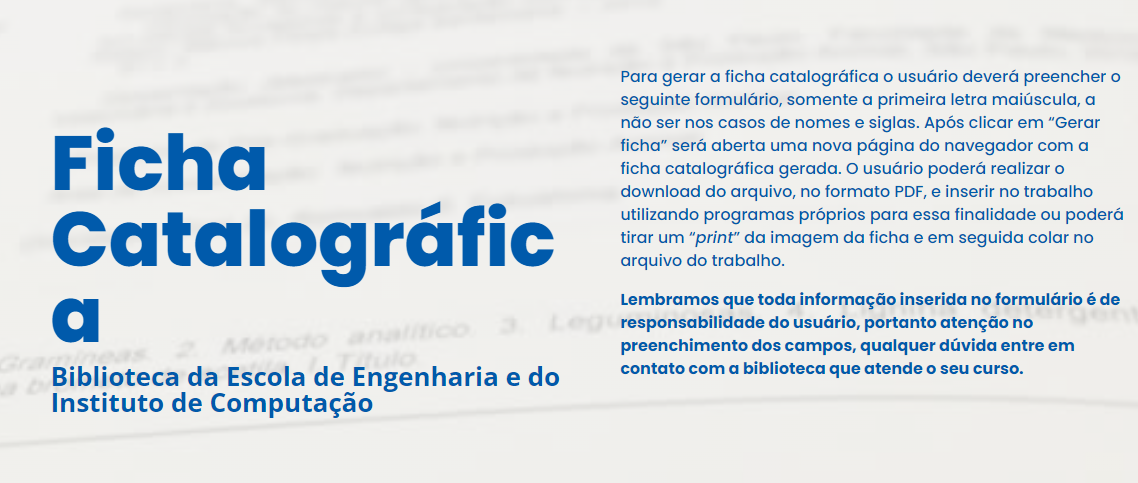
\includegraphics[width=1\linewidth]{capitulos/figuras/ficha_catalografica.png}
%   \caption{Ficha catalográfica}
% \end{figure}

% \cleardoublepage


% \pagestyle{ruledheader}
% \setcounter{page}{1}
% \pagenumbering{roman}

% --- -----------------------------------------------------------------
% --- Termo de aprovação. (Obrigatório)
% --- ----------------------------------------------------------------
\cleardoublepage
\thispagestyle{empty}

\vspace{-60mm}

\begin{center}
   {\large PAULO CEZAR LACERDA NETO}\\
   \vspace{7mm}

   APRENDIZADO PROFUNDO COMBINANDO REDES CONVOLUCIONAIS COM REDES RECORRENTES E TRANSFORMERS PARA APOIO AO DIAGNÓSTICO DA COVID-19 BASEADO EM TOMOGRAFIA COMPUTACIONAL DE TÓRAX\\
  \vspace{10mm}
\end{center}

\noindent
\begin{flushright}
\begin{minipage}[t]{10cm}
Proposta de Tese de Doutorado apresentada ao Programa de P\'{o}s-Gradua\c{c}\~{a}o em Computa\c{c}\~{a}o da Universidade Federal Fluminense como requisito parcial para a obten\c{c}\~{a}o do \mbox{Grau} de Doutor em Computa\c{c}\~{a}o. \'{A}rea de concentra\c{c}\~{a}o: \mbox{VIS\~{A}O COMPUTACIONAL} %preencha com a sua área de concentração

\end{minipage}
\end{flushright}
\vspace{0.5 cm}
\noindent
Maio de 2022. \\
\begin{flushright}
 % \parbox{11cm}
  {
  \begin{center}
  BANCA EXAMINADORA \\
  \vspace{5mm}
  \rule{11cm}{.1mm} \\
    Prof. Célio Vinicius Neves de Albuquerque - Orientador, UFF \\
    \vspace{3mm}
  \rule{11cm}{.1mm} \\
    Prof. Aura Conci, Co-orientadora, UFF\\
    \vspace{3mm}
  \rule{11cm}{.1mm} \\
    Prof. Anselmo Cardoso de Paiva, UFMA\\
  \vspace{3mm}
  \rule{11cm}{.1mm} \\
    Prof. Aristófanes Corrêa Silva, UFMA\\
    \vspace{3mm}
  \rule{11cm}{.1mm} \\
    Profa. Aline Marins Paes Carvalho, UFF\\
  \vspace{3mm}
  \end{center}
  }
\end{flushright}
\begin{center}
  \vspace{3mm}
  Niter\'{o}i \\
  2022

\end{center}

% --- -----------------------------------------------------------------
% --- Dedicatoria.(Opcional)
% --- -----------------------------------------------------------------
\cleardoublepage
\thispagestyle{empty}
\vspace*{200mm}

\begin{flushright}
{\em 
    Dedico esse trabalho a minha família por todo o seu apoio.
}
\end{flushright}
\newpage


% --- -----------------------------------------------------------------
% --- Agradecimentos.(Opcional)
% --- -----------------------------------------------------------------
\pretextualchapter{Agradecimentos}
\hspace{5mm}
Ao meu orientador e minha orientadora, que me mostraram os caminhos a serem seguidos e pela confiança depositada.



% --- -----------------------------------------------------------------
% --- Resumo em português.(Obrigatório)
% --- -----------------------------------------------------------------
\begin{resumo}


A pandemia da COVID-19 ocasionou milhões de casos da doença por todo o mundo, causada pelo coronavírus denominado SARS-CoV-2, gerando uma situação de emergência de saúde pública de âmbito mundial. 

Este trabalho propõe o desenvolvimento de um novo método para apoiar o diagnóstico de COVID-19, utilizando técnicas de processamento de imagens e aprendizado profundo aplicadas na análise de imagens médicas, mais especificamente imagens de tomografia computadorizada de tórax. A ideia é que o método possa ser utilizado por radiologistas para apoiar um diagnóstico rápido e eficaz da doença, reduzindo o impacto da COVID-19 e de outras doenças pulmonares no sistema de saúde. A metodologia do trabalho se baseia na construção de modelos  de aprendizado profundo, através da utilização de bases de dados públicas para treinamento de redes neurais convolucionais, em conjunto com técnicas de processamento de imagens, redes neurais recorrentes ou redes \textit{transformers} para a tarefa de classificação de imagens. O resultado esperado é que a abordagem proposta seja capaz de realizar as inferências em tempo real, com baixo custo e com resultados melhores do que outros métodos de última geração, em pelo menos uma das seguintes métricas: Sensibilidade, Especificidade, F1 Score e Área sob a Curva ROC.

{\hspace{-8mm} \bf{Palavras-chave}}: COVID-19; Aprendizado Profundo; Redes neurais convolucionais; Redes neurais recorrentes; Transformers; Diagnóstico auxiliado por computador

\end{resumo}

% --- -----------------------------------------------------------------
% --- Resumo em língua estrangeira.(Obrigatório)
% --- -----------------------------------------------------------------
\begin{abstract}

The COVID-19 pandemic caused by a virus called SARS-CoV-2, yielded millions of cases, provoking a public health emergency of international dimensions.

This work addresses the development of a method for analyzing medical images using image processing and deep learning techniques. The work methodology is based on the building of deep learning models, through the use of public databases for training convolutional neural networks, together with image processing techniques, recurrent neural networks, or \textit{transformers} networks for the classification task. The expected result is the proposed approach capable of making inferences in real-time, with the best results of other state-of-the-art methods, in at least one of the following measures: Sensitivity, Specificity, F1 Score, and Area under a ROC Curve.



{\hspace{-8mm} \bf{Keywords}}: COVID-19; Deep Learning; Convolutional neural networks; Recurrent neural networks; Transformers; Computer aided diagnostics.

\end{abstract}

% --- -----------------------------------------------------------------
% --- Lista de figuras.(Opcional)
% --- -----------------------------------------------------------------
%\cleardoublepage
\listoffigures



% --- -----------------------------------------------------------------
% --- Lista de tabelas.(Opcional)
% --- -----------------------------------------------------------------
\cleardoublepage
%\label{pag:last_page_introduction}
\listoftables
\cleardoublepage

% --- -----------------------------------------------------------------
% --- Lista de abreviatura.(Opcional)
%Elemento opcional, que consiste na relação alfabética das abreviaturas e siglas utilizadas no texto, seguidas das %palavras ou expressões correspondentes grafadas por extenso. Recomenda-se a elaboração de lista própria para cada %tipo (ABNT, 2005).
% --- ----------------------------------------------------------------

\cleardoublepage
% \printglossary[type=\acronymtype,title={Lista de Abreviaturas e Siglas}]
\pretextualchapter{Lista de Abreviaturas e Siglas}
\begin{tabular}{lcl}
AUC & : & \textit{Area Under ROC Curve};\\
CAD & : & \textit{Computer-Aided Diagnosis};\\
CNN & : & \textit{Convolutional Neural Network};\\
COVID-19 & : & \textit{Coronavirus Disease 2019};\\
GAP  & : & \textit{Global Average Pooling};\\
HPO & : & \textit{Hyperparemeter Optimization};\\
LSTM & : & \textit{Long Short-term Memory};\\
NIAB & : & \textit{Non-stochastic Infinite-armed Bandit};\\
PMC & : & Perceptron Multicamadas;\\
ReLU & : & \textit{Rectified Linear Activation Unit};\\
RNN & : & \textit{Recurrent Neural Network};\\
ROC & : & \textit{Receiver Operating Caracteristic};\\
RT-PCR & : & \textit{Reverse-Transcription Polymerase Chain Reaction};\\
SARS-Cov2 & : & \textit{Severe Acute Respiratory Syndrome Coronavirus 2};\\
TC & : & Tomografia Computadorizada;\\

\end{tabular}
\cleardoublepage


% --- -----------------------------------------------------------------
% --- Sumario.(Obrigatório)
% --- -----------------------------------------------------------------

\pagestyle{ruledheader}
\tableofcontents
\pagebreak %na pasta capítulos

% --- -----------------------------------------------------------------
% --- Inserção dos capítulos.
% --- todos os arquivos estão na pasta capítulos
% --- -----------------------------------------------------------------

\setcounter{page}{1} %parâmetros da contagem de paginas.
\pagenumbering{arabic} %padrão de números de paginas em arábico (1,2,3) 
\setcounter{page}{12} %inicia a contagem das paginas 12 - folha de rosto e considera a pagina da 

\pagestyle{ruledheader}
\chapter{Introdução} \label{cap:cap_introducao}

Em março de 2020 foi declarada a pandemia global da SARS-Cov2 pela Organização Mundial da Saúde~\cite{world2020director} e desde então um grande número de casos e mortes confirmaram o seu impacto em escala mundial \cite{WorldHealthOrganization2020CoronavirusReports}. O teste RT-PCR, do inglês \textit{Reverse-Transcription Polymerase Chain Reaction}, é considerado o padrão ouro para o diagnóstico da COVID-19 \cite{oliveira2020sars}.

No entanto estudos mostram que a tomografia computadorizada também tem papel importante no manejo de casos suspeitos de COVID-19 \cite{he2020diagnostic}, apresentando alta especificidade e valor preditivo positivo para o diagnóstico de COVID-19 \cite{santos2020initial}. Este exame tem um papel importante principalmente nos casos que apresentaram resultado negativo inicial no RT-PCR \cite{fang2020sensitivity}, sobretudo levando em consideração os pacientes que estão fora da janela ideal de coleta de amostras \cite{fonseca2021tomografia}. Enquanto que o RT-PCR tem desempenho modesto na medida de sensibilidade (53-88\%) \cite{kovacs2020sensitivity}. A sensibilidade e precisão de nível humano de TC para diagnóstico da COVID-19 são 97\% e 72\%, respectivamente \cite{caruso2020chest}. 

Para minimizar o risco de resultados de falso-negativos do teste RT-PCR, a TC de tórax pode ser aplicada em pacientes com suspeita clínica com resultado inicial negativo \cite{he2020diagnostic}. Vale notar que comparada à radiografia torácica, outro exame de imagem também utilizado para ajudar na detecção da doença, a tomografia computadorizada de tórax é mais sensível na detecção da COVID-19, bem como no monitoramento da progressão da doença \cite{wong2020frequency}.

Imagens médicas são elementos importantes para o diagnóstico de doenças. O diagnóstico assistido por computador, ou \textit{Computer Aided Diagnostics} (CAD), evoluiu bastante nos últimos anos, juntamente com a capacidade de processamento dos computadores, e o surgimento das técnicas de aprendizado profundo \cite{goodfellow2016deep}.  Atualmente a utilização de CNNs aplicada ao diagnóstico em cenários específicos já alcança desempenhos equiparáveis a especialistas em radiologia \cite{gulshan2016development, esteva2017dermatologist}.

Dado a magnitude dos efeitos da pandemia na sociedade, a pesquisa na área de diagnóstico da COVID-19 auxiliado por computador é de grande importância para desenvolvimento de novos métodos para diagnóstico que possam ser adotados pelos sistemas de saúde de todo o mundo na detecção e tratamento da doença. Embora já existam estudos com foco no uso de aprendizado profundo para apoiar o diagnóstico de COVID-19 utilizando tomografias, há espaço para melhorar o desempenho das técnicas publicadas até o momento da escrita deste texto, como por exemplo na sensibilidade da detecção da doença a fim de reduzir ainda mais o número de resultados falso-negativos e, consequentemente, aumentar a chance de detecção e tratamento bem-sucedidos da COVID-19.

\section{Hipóteses de Pesquisa}\label{sec:obj_perg_hipoteses}

Este trabalho analisa a utilização de redes neurais convolucionais \cite{lecun1990handwritten} combinadas com redes neurais recorrentes \cite{Rumelhart1986} ou \textit{transformers} \cite{vaswani2017attention} na detecção da COVID-19 em exames de tomografia computadorizada de tórax. A combinação de redes CNN e LSTM já foi realizada com sucesso em exames de ultrassom \cite{barros2021pulmonary}. O objetivo é verificar que o desempenho destas redes quando combinadas apresenta um desempenho igual ou superior ao especialista humano ou outras técnicas que aplicam primariamente redes neurais convolucionais para a detecção da COVID-19 em relação a sensibilidade.

Assim, a hipótese dessa pesquisa pode ser apresentada da seguinte forma: 

"A aplicação de redes neurais convolucionais combinadas com redes neurais recorrentes ou transformers constituem uma forma mais eficaz na detecção da COVID-19 em tomografias computadorizadas de tórax quando comparadas com o desempenho humano e com a utilização apenas de redes neurais do tipo convolucionais."

\section{Objetivos}\label{sec:obj_trabalho}

O objetivo geral desta tese é propor e avaliar um novo método para detecção da COVID-19 utilizando aprendizado profundo, através da extração de características espaciais e sequenciais de estudos de tomografia de tórax. 

Para alcançar o objetivo geral, os seguintes objetivos específicos são estabelecidos: 
\begin{itemize}
  
  \item Desenvolver técnicas de preparação de imagens com o objetivo de evidenciar as informações relevantes para o aprendizado das redes neurais relacionado a COVID-19.
  
  \item Propor técnicas de preprocessamento das imagens para aumento dos dados de forma a melhorar a capacidade de generalização das redes e reduzir o viés por conta do conjunto de dados utilizado.
  
  \item Propor técnica aplicando redes neurais convolucionais combinadas com redes neurais recorrentes na tarefa de classificar exames de tomografia computadorizada de tórax como COVID-19 ou não COVID-19.
  
  \item Propor técnica aplicando redes neurais convolucionais combinadas com redes neurais \textit{transformers} na tarefa de classificar exames de tomografia computadorizada de tórax como COVID-19 ou não COVID-19.  
  
  \item Aplicar técnica de otimização do conjunto dos hiperparâmetros a serem empregados na definição da arquitetura e treinamento das redes neurais utilizadas nesta pesquisa.
  
%   \item Propor técnica de detecção de lesões ocasionadas pela COVID-19 com base em TC, para uso combinado com o classificador da doença, fornecendo mais informações para apoiar o diagnóstico realizado pelo médico.
  
  \item Avaliar o método proposto através de experimentos usando uma base de imagens públicas de tomografias computadorizadas, a partir de medidas de desempenho usualmente utilizadas para avaliar classificadores baseados em aprendizado profundo.
  
  \item Comparar o desempenho do método proposto com outros métodos publicados na literatura.
  
\end{itemize}

\section{Estrutura do Trabalho}\label{sec:cap_introducao_est_trabalho}

Esta proposta de tese está organizada da seguinte forma: No  Capítulo \ref{cap:cap_fundamentos}  são apresentados conceitos que são fundamentais para aplicação da técnica proposta, no Capítulo \ref{cap:cap_trabalhos} são comentados alguns métodos publicados recentemente relacionados a aplicação de aprendizado profundo para diagnóstico da COVID-19, no Capítulo \ref{cap:cap_metodo} é descrito em detalhes o método proposto por este trabalho, no Capítulo \ref{cap:cap_resultados} os resultados preliminares dos experimentos são apresentados e discutidos. Finalmente, o Capítulo \ref{cap:cap_planejamento} apresenta o planejamento, as limitações do estudo até o momento da qualificação, e as contribuições esperadas com a tese de doutorado.

% \section{Notação Utilizada}\label{sec:cap_introducao_notacao}

% Durante o texto são utilizadas letras, símbolos para representar elementos matemáticos como variáveis e equações. Como convenção as variáveis são representadas com letras minusculas e em itálico e para algumas delas são utilizadas letras do alfabeto grego, como por exemplo na equação \ref{eq:z_score_exemplo} que descreve o cálculo do \textit{z-score} para normalização dos \textit{pixels} de uma imagem, neste equação a letra $z$ representa a nova intensidade do \textit{pixel}, $x$ corresponde ao seu valor original, e $\mu$ e $\sigma$ equivalem respectivamente a média e desvio padrão dos \textit{pixels} da imagem.

% \begin{equation} \label{eq:z_score_exemplo}
% z = \frac{x - \mu }{\sigma}
% \end{equation}

% Assim como as variáveis, os vetores utilizados na descrição do funcionamento das redes neurais também são representados como letras minúsculas em itálico, já as matrizes são representadas por letras maiúsculas em itálico. Elementos de um vetor são representados com a notação $x_i$ que no caso corresponde ao \textit{i}-ésimo elemento do vetor \textit{x}. 

% Ainda relacionado a representação das redes neurais, componentes de uma determinada camada da rede neural são representados com sobrescrito entre colchetes, por exemplo, de acordo com essa notação a expressão $W^{[l]}$ pode ser usada para representar a matriz com os pesos da camada $l$ de uma rede neural.

% Quando necessário representar os elementos de um conjunto de dados, é utilizada a notação $x^{(i)}$ para representar o vetor correspondente a \textit{i}-ésima amostra de um conjunto de dados X.



\pagestyle{ruledheader}
\chapter{Fundamentação Teórica} \label{cap:cap_fundamentos}

Neste capítulo são apresentados de forma resumida os fundamentos que formam a base desta pesquisa: o aprendizado profundo e os tipos de rede neurais aplicados neste trabalho, assim como informações gerais sobre a COVID-19 e os achados típicos encontrados nos exames de imagem de tomografia de tórax de pacientes com esta doença.

Na seção a seguir sobre aprendizado profundo o objetivo é  expor ao leitor os conceitos gerais sobre cada um dos temas apresentados, porém para um conteúdo mais abrangente sobre os temas recomenda-se duas publicações sobre o tema aprendizado profundo: \cite{goodfellow2016deep} e \cite{zhang2020dive}.

\section{Aprendizado Profundo}\label{section:cap_fundamentos_dl}

O aprendizado profundo \cite{goodfellow2016deep} é um tipo de aprendizado de máquina que obtém grande poder e flexibilidade ao representar o conhecimento como uma hierarquia de conceitos aninhados, com cada conceito definido em relação a conceitos mais simples.

Para ilustrar a ideia, a Figura \ref{fig:fun_modelo_aprendizado_profundo} apresenta um modelo de aprendizado profundo com ênfase em imagens. Conforme a ilustração, o aprendizado profundo é capaz de representar conceitos mais abstratos como um cachorro, dividindo o conceito em uma série de conceitos mais simples, cada um descrito por uma camada diferente do modelo. 

É importante comentar que para ter aplicação prática uma rede neural apresentaria mais camadas do que exibido na Figura \ref{fig:fun_modelo_aprendizado_profundo}, um exemplo simplificado apenas para fins ilustrativos. 

Os dados de entrada são transmitidos para a camada de entrada, a camada observável, pois contém as variáveis visíveis de entrada do modelo. No exemplo da Figura \ref{fig:fun_modelo_aprendizado_profundo} a camada visível recebe como entrada as intensidades dos \textit{pixels} da imagem.

Em seguida, uma série de camadas ocultas extraem características cada vez mais abstratas da imagem. Essas camadas são chamadas de “ocultas”, pois têm uma resposta não observável, mas sim latente e a saída de cada camada deve determinar quais conceitos são úteis para explicar os relacionamentos nos dados que recebeu de entrada.

Ainda no exemplo da Figura \ref{fig:fun_modelo_aprendizado_profundo}, na primeira camada oculta, a partir dos \textit{pixels} da imagem de entrada, são determinadas as bordas presentes na imagem, comparando o brilho dos \textit{pixels} vizinhos. A partir das bordas representadas pela primeira camada oculta, a segunda camada oculta determina cantos e contornos, identificados a partir da combinação das arestas. 

Com base na representação da imagem da segunda camada oculta, em termos de cantos e contornos, a terceira camada oculta é capaz de representar partes de objetos específicos, que correspondem a combinações particulares de contornos e cantos. 

Finalmente, esta descrição da imagem em termos das partes do objeto que ela contém, pode ser usada para classificar a imagem. 

\begin{figure}[!ht]
\centering
\includegraphics[width=1.0\linewidth]{capitulos/figuras/fun_modelo_aprendizado_profundo.pdf}
\caption{Um modelo de aprendizado profundo.}
\label{fig:fun_modelo_aprendizado_profundo}
\end{figure}

Embora não exista um consenso sobre quanta "profundidade" um modelo requer para se qualificar como “profundo”, o aprendizado profundo pode ser considerado como o estudo de modelos que envolvem uma quantidade maior de composição de funções ou conceitos aprendidos do que o aprendizado de máquina tradicional.

Uma rede neural é um modelo inspirado no cérebro, composto por camadas formadas por neurônios. Os modelos de aprendizado profundo são redes neurais contendo múltiplas camadas ocultas, também chamadas de redes neurais profundas. 

Com o propósito de facilitar a leitura e padronizar a nomenclatura utilizada no texto, daqui em diante será utilizado simplesmente o termo rede neural para se referir a modelos de aprendizado profundo.

Nas próximas subseções são apresentados os quatro tipos de redes neurais utilizadas nesta pesquisa, assim como a técnica de otimização de hiperparâmetros de redes neurais.

\subsection{Perceptron Multicamadas}\label{subsec:cap_fundamentos_ann}

As redes Perceptron Multicamadas (PMC) são uma forma clássica de rede neural, elas têm esse nome pois seus neurônios são inspirados na Perceptron\cite{rosenblatt:58}, uma forma simples de rede neural com um único neurônio.

Uma PMC tem sua estrutura formada por uma camada de entrada, uma de saída e entre elas, uma ou mais camadas ocultas. Cada camada apresenta um conjunto de unidades lógicas, no caso das camadas ocultas estas unidades são os neurônios da rede.

A camada de entrada apresenta um número de unidades de entrada, cada uma delas recebe as características do item que se deseja processar na rede. Em uma rede voltada para classificar um paciente de acordo com uma doença, por exemplo, a camada de entrada pode receber como entrada um vetor contendo características como a idade do paciente, o sexo e assim por diante.

A camada de saída apresenta unidades cuja quantidade é definida pelo problema que a rede resolve, por exemplo, no caso de uma classificação multi-classe é utilizada uma saída para cada uma das classes que a rede conhece.

As camadas ocultas têm esse nome, pois ficam "escondidas" entre a camada de entrada e a de saída, cada camada oculta é formada por um conjunto de neurônios e cada um deles recebe como entrada a saída de cada unidade da camada anterior. Essas redes são ditas completamente conectadas, pois cada unidade em uma camada é conectada a todas as unidades da próxima camada. Uma camada de uma rede completamente conectada recebe igualmente esta denominação, e também é referenciada como camada densa.

O comportamento de cada neurônio segue um padrão simples, ele recebe como entrada todas as saídas da camada anterior, seja uma camada oculta ou a camada de entrada. Na sequência ele realiza a soma ponderada dos valores de entrada com pesos e adiciona um viés. Ao final aplica uma função não linear, também conhecida como função de ativação, para calcular o valor de saída. 

O funcionamento de um neurônio da PMC pode ser descrito pela Equação \ref{eq:fun_neuronio_pmc_vector}, considerando que a camada anterior tem tamanho $n$, ele recebe como entrada o vetor coluna $x$ de tamanho 3x1. O escalar $a$ corresponde ao valor de saída, enquanto que o vetor $w$ e o escalar $b$ simbolizam respectivamente os pesos e o viés. A função de ativação é representada pela letra grega $\varphi$. Os vieses e pesos de uma rede neural correspondem ao número de parâmetros da rede.

\begin{equation}
    a = \varphi(\sum_{i}^{n}w_ix_i+b)
\label{eq:fun_neuronio_pmc_vector}
\end{equation}

A Figura \ref{fig:fun_neuronio_pmc} ilustra o comportamento do neurônio, conforme descrito anteriormente, recebendo como entrada um vetor $x$ de tamanho 3.

\begin{figure}[!ht]
\centering
\includegraphics[width=0.5\linewidth]{capitulos/figuras/fun_neuronio_pmc.pdf}
\caption{Neurônio da rede perceptron multicamadas.}
\label{fig:fun_neuronio_pmc}
\end{figure}

É interessante notar que nas redes neurais, são utilizadas funções de ativação não lineares, como a unidade linear retificada (ReLU), a sigmóide ou a tangente hiperbólica, com o intuito de introduzir não linearidade nas redes e produzir funções capazes de separar dados não linearmente separáveis. Para permitir o treinamento da rede com o método Gradiente Descendente Estocástico \cite{robbins1951stochastic}, essas funções devem ser deriváveis, mesmo que em parte, como no caso da ReLU que não é derivável quando $x=0$.

A Figura \ref{fig:fun_pmc} ilustra uma rede PMC composta da camada de entrada, duas camadas ocultas e a camada de saída. Na notação utilizada $x_i$ corresponde ao i-ésimo item do vetor de entrada $x$, enquanto ${a_i}^{[l]}$ representa o resultado da função de ativação do i-ésimo neurônio da camada $l$, a letra grega $\varphi^{[l]}$ corresponde a função de ativação da camada $l$, ao passo que ${w_{ij}}^{[l]}$ representa o peso aplicado a j-ésima entrada da i-ésima unidade da camada \textit{l}, já o termo ${b_i}^{[l]}$ equivale ao viés utilizado na i-ésima unidade da camada \textit{l} e por fim $\hat{y}$ simboliza o resultado da função de ativação da camada de saída da rede.

\begin{figure}[!ht]
\centering
\includegraphics[width=1.0\linewidth]{capitulos/figuras/fun_pmc.pdf}
\caption{Rede perceptron multicamadas.}
\label{fig:fun_pmc}
\end{figure}


A operação realizada por uma camada da PMC pode ser representada de maneira simplificada na forma vetorial: $a^{[l]} = \varphi (W^{[l]^T}a^{[l-1]} + b^{[l]})$. Em que $a$ é o vetor com todas as saídas das unidades da camada $l$, $\varphi$ corresponde a função de ativação da camada $l$, os pesos da camada $l$ são representados por uma matriz $W^{[l]}$ já que cada par de unidades em duas camadas consecutivas apresenta um peso correspondente, $a$ é o vetor com os valores das ativações da camada anterior. Os vetores mencionados anteriormente são vetores do tipo coluna. A matriz de pesos é transposta para permitir a multiplicação de $W^{[l]}$ pelo vetor de entrada $a^{[l-1]}$. O vetor $b$ contém o viés de todas as unidades da camada $l$.


\subsection{Redes Neurais Convolucionais}\label{subsec:cap_fundamentos_cnn}

As redes neurais convolucionais \cite{lecun1990handwritten} geralmente são aplicadas em problemas relacionados à área de visão computacional. Inicialmente foram propostas para resolver problemas de classificação de imagens, porém atualmente apresentam tipos diferentes de aplicações nesta área, como por exemplo: detecção de objetos, transferência de estilo e segmentação de imagens. Devido ao desempenho superior deste tipo de rede em desafios de classificação de imagens \cite{russakovsky2015imagenet}, essas redes representam o estado da arte neste tipo de aplicação. 

Uma rede neural convolucional ou CNN, do inglês \textit{Convolutional Neural Network} é baseada em operações de convolução, que correspondem a aplicação de filtros (\textit{kernels}) que realçam determinadas características da imagem. Para que seja possível compreender melhor a aplicação desses filtros usando a operação de convolução, é necessário entender o que é convolução.

A convolução é um operador matemático linear, que a partir de dois sinais (imagem e filtro) resulta em um terceiro sinal (a representação da imagem). A convolução discreta consiste em operações simples de multiplicações e somas, comumente utilizada em processamento de sinais e imagens. O objetivo é calcular a soma do produto desses sinais ao longo da região de superposição de sinais, mediante o deslocamento existente entre eles. Em processamento de imagens a convolução é usada, por exemplo, para detecção de arestas horizontais e verticais.

A Figura \ref{fig:fun_convolucao} representa o procedimento de convolução na matriz de tamanho 3x3 do lado esquerdo com o filtro representado pela matriz de tamanho 2x2 representada no meio da figura, resultando na matriz de saída no lado direito. O filtro desliza sobre a matriz de entrada no sentido da esquerda para direita e de cima para baixo, a cada posição do filtro é realizada a soma dos produtos entre cada elemento da matriz de entrada que está sobreposto com o elemento correspondente do filtro que o sobrepõe, o resultado é armazenado em uma célula correspondente na matriz de saída. Na Figura \ref{fig:fun_convolucao} a operação de multiplicação e soma de uma posição da convolução está destacada em azul.

\begin{figure}[!ht]
    \centering
    \includegraphics[width=0.7\linewidth]{capitulos/figuras/fun_convolucao.pdf}
    \caption{Exemplo da convolução de uma imagem 3x3 por um filtro 2x2.}
    \label{fig:fun_convolucao}
\end{figure}

A ideia por trás das convoluções é transformar a imagem, extraindo as características relevantes para o problema que ser quer resolver. Quando sucessivas operações de convolução são aplicadas ao longo das camadas convolucionais é possível extrair características cada vez mais abstratas e ao mesmo tempo diminuir o tamanho da imagem resultante. Por consequência essa construção hierárquica também reduz a quantidade de parâmetros envolvidos no treinamento, o que é uma grande vantagem sobre as PMCs.

As características extraídas das imagens são invariantes à posição da imagem, de forma que são capazes de assimilar padrões espaciais que podem ser aprendidos e  reutilizados em diferentes partes das imagens. Uma aresta vertical, por exemplo, é uma característica que pode ser facilmente reutilizada. Além disso, devido à convolução, as conexões da rede tornam-se esparsas, ou seja, cada saída depende somente de uma pequena quantidade de parâmetros da entrada \cite{zhang2020dive}.

Uma CNN tem sua estrutura tipicamente formada por uma camada de entrada, uma de saída e entre elas uma ou mais camadas convolucionais e uma ou mais camadas densas ao final da rede. Também é comum utilizar camadas de agrupamento e ou de normalização em lote após cada camada convolucional.

A camada de entrada da CNN recebe a imagem a ser processada pela rede, em geral uma matriz de três dimensões: largura, altura e profundidade. A profundidade corresponde aos canais de cores da imagem, por exemplo, imagens coloridas usualmente tem três canais enquanto imagens em tons de cinza apresentam um canal apenas.

A camada de convolução é a principal camada da CNN, ela é formada por filtros, matrizes quadradas em que cada um dos elementos representa um peso utilizado na operação de convolução. Assim como nas redes PMC, após a função linear, que no caso da CNN corresponde a operação de convolução somada do viés, é aplicado ao resultado uma função não linear como a ReLU. A cada filtro utilizado na convolução é gerado uma mapa de ativação, uma matriz de duas dimensões, de modo que a saída da camada de convolução é um volume com largura, altura e profundidade, em que a última dimensão corresponde ao número de filtros aplicados na camada. Os valores de cada elemento dos filtros e os vieses da camada de convolução formam os parâmetros desta camada.

A camada de agrupamento tem como finalidade subamostrar a imagem de entrada para reduzir a carga computacional, reduzindo progressivamente o tamanho da saída das camadas convolucionais cada vez que a camada de agrupamento é aplicada após cada camada de convolução, ajudando a reduzir o número de parâmetros da rede.

A camada de normalização em lote, proposta por \cite{ioffe2015batch} adiciona à rede uma operação de normalização após a camada convolucional. A operação centraliza a média em zero e normaliza a saída da camada convolucional que será utilizada de entrada na próxima camada. A utilização da normalização em lote traz algumas vantagens: ajuda no problema de desaparecimento do gradiente, ou \textit{vanishing gradient problem}; as redes ficam menos sensíveis à inicialização dos pesos; funciona como um regularizador da rede ajudando no problema do sobreajuste. Além de todas estas vantagens, segundo os autores da técnica, quando utilizada em uma rede para classificação de imagens, a normalização em lote permite a rede alcançar a mesma acurácia com 14 vezes menos etapas de treinamento da rede.

As CNNs em geral apresentam uma ou duas camadas densas ao final, antes da camada densa de saída. A última camada apresenta uma função de ativação adequada para o problema que a rede resolve, no caso de uma classificação multiclasse, por exemplo é utilizada uma função de ativação como a Softmax. A saída da última camada convolucional da rede precisa ser "achatada" para servir de entrada para a camada densa, esse procedimento basicamente formata a matriz multidimensional da saída da camada convolucional em um vetor coluna, sem alteração nos valores dos elementos de saída. Outra forma também utilizada para o achatamento da saída da camada convolucional em um vetor coluna é através do uso de uma camada de agrupamento médio global do inglês \textit{Global Average Pooling} (GAP) \cite{lin2013network}, que gera o vetor coluna em que cada elemento corresponde a média de cada mapa de ativação apresente na saída da camada de convolução anterior.

Muitas arquiteturas de redes CNN foram propostas nos últimos tempos, embora todas sejam baseadas nas camadas convolucionais, cada arquitetura apresenta diferentes composições em termos de número e tipos de camadas. Algumas das mais populares são a LeNet \cite{lecun1998gradient},  Inception \cite{szegedy2017inception}, Xception \cite{Chollet2017},  ResNet \cite{he2016deep}, DenseNet \cite{huang2017densely}, VGG16 \cite{simonyan2014very}, NASNet \cite{zoph2018learning}, EfficientNet \cite{tan2019efficientnet} e MobileNet \cite{Sandler2018}.

Para exemplificar o funcionamento das redes neurais convolucionais, na Figura \ref{fig:fun_cnn_lenet} é apresentada a rede Lenet, mais especificamente a versão Lenet-5. Esta rede foi criada com o propósito de classificar dígitos manuscritos e é composta de duas camadas de convolução, cada uma delas seguida de uma camada de agrupamento, seguidas por mais uma camada de convolucão e por fim duas camadas densas, sendo a última delas a camada de saída em que é aplicada a função de ativação Softmax para classificação dos dígitos. 

\begin{figure}[!ht]
\centering
\includegraphics[width=1.0\linewidth]{capitulos/figuras/fun_cnn_lenet.pdf}
\caption{Estrutura da rede LeNet-5.}
\label{fig:fun_cnn_lenet}
\end{figure}

\subsection{Redes Neurais Long Short-Term Memory (LSTM)}\label{subsec:cap_fundamentos_lstm}

Tanto as redes neurais perceptron multicamadas quanto as convolucionais são redes do tipo \textit{feedforward}, redes em que o processamento ocorre somente em uma direção, ou seja, da camada de entrada para a camada de saída. Elas recebem uma entrada e processam essa informação ao longo de suas camadas de uma forma direta para gerar um resultado na saída. Dado este comportamento, as redes \textit{feedforward} não são as mais indicadas para tratar dados sequenciais ou séries temporais, em que a informação de um momento anterior é relevante para a predição em um momento posterior, como um filme, que corresponde a uma sequência de imagens, ou um texto que é uma sequência de palavras, só para citar alguns exemplos. Para trabalhar com informações sequenciais foram criadas as redes neurais recorrentes, ou RNNs \cite{Rumelhart1986}.

As redes neurais recorrentes são assim chamadas porque seus neurônios realizam a mesma tarefa recorrentemente para cada elemento de uma sequência, de forma que a saída de cada neurônio é dependente do cálculo realizado com base no elemento anterior da sequência e armazenado em sua memória interna. Para utilizar a informação sequencial presente nos dados, durante o treinamento da rede, a LSTM, tipo de rede recorrente, usa como entrada de cada neurônio, além do dado de entrada, a saída do mesmo neurônio obtida com o dado do passo anterior da sequência. Dessa forma ele recebe não apenas novas entradas a cada passo da sequência, mas também adiciona a estas entradas a saída da entrada anterior.

Diferente das redes PMCs ou CNNs, as RNNs mantém a informação de estado, em memória, de modo que as futuras entradas da rede são derivadas das saídas anteriores. Este efeito de "memória" é obtido através de conexões recorrentes, que funcionam como um laço (\textit{loop}) interno na rede que a cada iteração processa um elemento. 

A Figura \ref{fig:fun_rnn_neuronio} demonstra de forma simplificada o conceito de um neurônio de uma camada de uma rede neural recorrente. No exemplo é ilustrado um único neurônio que recebe uma entrada $x$ que corresponde a uma série temporal com três passos de tempo. Na parte superior
é representado o neurônio com a entrada, a saída $\hat{y}$ e a conexão recorrente, na parte inferior a ilustração deste neurônio "desenrolado" ao longo do tempo.

\begin{figure}[!ht]
\centering
\includegraphics[width=0.45\linewidth]{capitulos/figuras/fun_rnn_neuronio.pdf}
\caption{Neurônio recorrente se desenrolando ao longo do tempo.}
\label{fig:fun_rnn_neuronio}
\end{figure}

No diagrama desenrolado da Figura \ref{fig:fun_rnn_neuronio}, cada neurônio tem duas saídas. Uma é a saída correspondente ao passo de tempo especifico que o neurônio está processando e a outra atua como entrada para o próximo neurônio funcionando como a "memória" do processamento dos passos de tempo anteriores.

As primeiras redes neurais recorrentes apresentaram um problema com o aprendizado de dependências de longo prazo, dificultando o trabalho com sequências longas, de forma que as informações nas primeiras entradas da sequência se perdem com o passar do tempo. A questão foi explorada em profundidade por \cite{hochreiter1997long} e \cite{bengio1994learning}. Para resolver o problema das RNNs com as dependências de longo prazo, foi proposta um novo tipo de rede recorrente chamada Long Short-Term Memory (LSTM) \cite{hochreiter1997long, zaremba2014recurrent, graves2005framewise}, que quer dizer memória longa de curto prazo. 

As redes neurais LSTM foram concebidas especificamente para evitar o problema de dependência de longo prazo. Lembrar-se de informações por longos períodos de tempo é parte do seu comportamento padrão. As Long Short-Term Memory (LSTM) são uma variante específica de Redes Neurais Recorrentes (RNN) que foram projetadas para evitar o problema do desaparecimento do gradiente, comum em RNNs tradicionais. A LSTM apresenta uma estrutura de "portas" que regulam o fluxo de informações, permitindo que a rede mantenha ou descarte informações ao longo do tempo. Isso permite que a LSTM seja capaz de aprender dependências de longo prazo e sequências de dados com maior eficácia. Essas características tornam as LSTMs particularmente úteis para tarefas que envolvem sequências de dados, como reconhecimento de voz, tradução automática e processamento de linguagem natural, além de tarefas com imagens. No entanto, apesar de seu desempenho impressionante nessas tarefas, as LSTMs podem ser computacionalmente intensivas e mais lentas para treinar em comparação com alguns modelos mais recentes, como os Transformers.

\subsection{Mecanismos de Atenção e Transformers}\label{subsec:cap_fundamentos_attention_transformers}

Mecanismos de atenção \cite{bahdanu2014} são componentes de redes neurais que aprendem a selecionar a parte das entradas que o restante do modelo deve focar em cada passo de tempo. Os mecanismos de atenção foram criados com foco na tradução de textos, porém evoluíram para aplicações com imagens, como por exemplo na geração de legendas automáticas para vídeos \cite{xu2015show}. Uma vantagem dos mecanismos de atenção é que eles permitem que o modelo capture relações de longo alcance entre os elementos da sequência, sem depender de estados ocultos intermediários.

Os \textit{Transformers} \cite{vaswani2017attention} são um tipo de rede neural que aplica mecanismos de atenção sem o uso de quaisquer camadas recorrentes, trazendo como vantagem um melhor desempenho em tempo de treinamento, pois são capazes de processar a sequência de entrada em paralelo, além de apresentarem resultados superiores em aplicações de processamento de linguagem natural \cite{wolf2016transformers}, superando os resultados obtidos nestas aplicações com redes neurais recorrentes e convolucionais. Alguns tipos de transformers publicados recentemente como ELMo \cite{Peters2018DeepRepresentations}, GPT \cite{radford2018improving} e BERT \cite{devlin2018bert} mostram o grande avanço obtido com esse tipo de rede em aplicações de processamento de linguagem natural. Além disso, os Transformers também têm mostrado potencial no processamento de imagens, sendo capazes de lidar com estruturas visuais complexas de maneira eficiente. A aplicação dessas redes em tarefas de visão computacional, como classificação de imagens e segmentação, tem apresentado resultados promissores, abrindo novas possibilidades para o uso de Transformers além do processamento de linguagem natural.
    
\subsection{Treinamento de uma Rede Neural}\label{subsec:cap_fundamentos_treinamento_ann}

A estrutura de uma rede neural tem atributos como o número de camadas, quantidade de neurônios e função de ativação de uma camada e assim por diante, esses atributos estruturais da rede são chamados de hiperparâmetros. Não confundir com os parâmetros da rede, formados pelos pesos e vieses dos neurônios. Os parâmetros da rede são "aprendidos" através de um processo de treinamento em que a rede aprende os parâmetros a partir de um conjunto de dados.

No caso do aprendizado profundo supervisionado, o treinamento é feito com base em um conjunto de dados com amostras cujo resultado é conhecido antecipadamente. No caso de uma tarefa de classificação por exemplos, cada amostra esta previamente rotulada com a classe correspondente. Antes de iniciar o treinamento de uma rede é necessário definir uma \textit{loss function} ou função de perda, uma função que mede a discrepância entre o valor de saída da rede e o valor esperado relativo a uma amostra. A função de perda é definida de acordo com a tarefa escolhida, na classificação multiclasse por exemplo, geralmente é utilizada a entropia cruzada, enquanto que o erro quadrático médio é normalmente a função utilizada em tarefas de regressão com valores contínuos. 

Com o objetivo de treinar uma rede neural, o conjunto de dados disponível para treinar a rede em geral é dividido em três conjuntos:  treinamento, validação e testes, embora existam algumas variações, como no caso da validação cruzada.  O conjunto de treinamento, como o próprio nome diz, é usado para treinar a rede, o que geralmente acontece utilizando-se o algoritmo de \textit{back-propagation} \cite{Rumelhart1986}.

No \textit{back-propagation}, cada amostra do conjunto de dados de treinamento é processada pela rede na etapa de \textit{forward} e o resultado utilizado para calcular o erro entre o valor esperado e o valor predito pela rede utilizando a função de perda. Na etapa de \textit{backward} os parâmetros da rede são ajustados com o intuito de reduzir o erro da rede. O ajuste dos parâmetros é realizado com base em um algoritmo de otimização, como por exemplo, o gradiente descendente, minimizando o erro entre as predições realizadas pela rede e os rótulos do conjunto de dados de treinamento.

O conjunto de dados de validação é usado para avaliar a rede durante o processo de treinamento, ajustar os hiperparâmetros e executar a seleção da rede, enquanto que o conjunto de testes é usado no final do projeto, a fim de avaliar o desempenho da rede final que foi ajustada e selecionada no processo de treinamento com base nos conjuntos de treinamento e validação.

A avaliação da rede é realizada com base em métricas escolhidas de acordo com a aplicação. As mais utilizadas geralmente são: acurácia, precisão, revocação ou \textit{recall}, F1 Score e a área sob a curva ROC, ou AUC. A acurácia é a fração que representa o total de predições corretas de todas as predições realizadas pela rede. A precisão é a fração de positivos verdadeiros entre os positivos preditos pela rede neural e o \textit{recall} representa a fração de positivos preditos pela rede do total de positivos verdadeiros. A área sob a curva ROC indica como a taxa de falsos positivos cresce à medida que a taxa de verdadeiros positivos aumenta. Por fim o F1 Score é calculado com base na média harmônica da precisão e \textit{recall}.

O aprendizado por transferência, ou \textit{transfer learning} é uma estratégia eficaz para treinar uma rede quando se tem um pequeno conjunto de dados. Nesta técnica geralmente a rede é pré-treinada em um conjunto de dados extremamente grande, como o ImageNet \cite{Russakovsky2014}, para depois ser reutilizada e aplicada à tarefa de interesse em que se tem poucos dados disponíveis. 

O aprendizado por transferência por extração de características em uma rede convolucional é o método em que as camadas densas de uma rede pré-treinada são removidas e a parte restante no início da rede, chamada base convolucional, é mantida. A parte preservada funciona como um extrator de características. Nesse método, uma ou mais camadas de rede são adicionadas ao topo da base convolucional e o conjunto final, formado pela base convolucional com seus pesos "congelados" e as camadas adicionais passam por um processo de treinamento, com base no conjunto de dados com menor tamanho. Neste processo, apenas os parâmetros da parte adicionada são "aprendidos".

Outra forma de aprendizado por transferência de redes convolucionais é conhecida como ajuste fino, em que não apenas são adicionadas novas camadas a uma base convolucional previamente treinada, mas também uma ou mais camadas na parte final da base convolucional são "descongeladas" para que tenham seus parâmetros também atualizados no processo de treinamento com o novo conjunto de dados.

\textit{Overfitting}, ou sobreajuste, é um fenômeno que ocorre comumente no processo de treinamento de redes neurais. Ele corresponde a situação em que a rede aprende perfeitamente os pesos com base no conjunto de treinamento, mas não consegue generalizar, e portanto, quando avaliada com base nos conjuntos de dados de validação ou testes, os resultados são insatisfatórios. Nas redes CNNs o sobreajuste pode ocorrer em casos em que os filtros da rede convolucional aprende padrões que não fazem parte do domínio do problema.

Nos casos em que há poucos dados para treinamento há um risco alto da rede ficar superajsutada para estes dados. Nesses casos, uma técnica útil para ajudar com este problema é chamada \textit{data augmentation}, ou expansão do conjunto de dados. Ela expande o conjunto de dados de treinamento, fazendo uma série de alterações aleatórias nas imagens para produzir exemplos de treinamento parecidos, mas ao mesmo tempo diferentes. A ideia é que exemplos de treinamento modificados aleatoriamente podem reduzir a dependência de uma rede com características específicas, melhorando assim sua capacidade de generalização, bem como reduzindo a risco de sobreajuste durante o treinamento. 

    
\subsection{Otimização de Hiperparâmetros (HPO)}\label{subsec:cap_fundamentos_hpo}

O desempenho de uma rede neural está diretamente relacionado ao seu treinamento \cite{riaz2020deep}, um processo no qual se busca aprender os melhores parâmetros da rede que minimizam uma função de perda, dado um conjunto de dados amostrais e seus rótulos correspondentes. Entretanto, antes do processo de treinamento, alguns parâmetros devem ser estabelecidos, como a arquitetura da rede neural, a taxa de aprendizado e o otimizador utilizado.

Esses parâmetros são conhecidos como hiperparâmetros e geralmente são definidos por engenheiros de aprendizado de máquina com base em sua experiência empírica e intuição \cite{choi2021active} desenvolvida ao longo do tempo. Para tornar o processo de seleção de hiperparâmetros mais eficiente, algumas técnicas de otimização de hiperparâmetros foram desenvolvidas ao longo do tempo, como o método Bayesiano~\cite{snoek2012practical} e a busca aleatória~\cite{bergstra2012random}.

Mais recentemente, um método de otimização conhecido como Hyperband \cite{Li2017} foi proposto. Este método define a otimização de hiperparâmetros como um problema de exploração pura não-estocástico de caça-niqueis com braços infinitos, do inglês \textit{pure-exploration non-stochastic infinite-armed bandit} (NIAB), um problema de decisão sequencial, onde, em cada estágio, um dos infinitos braços é escolhido e uma recompensa é obtida de acordo com a sequência escolhida.

O Hyperband tem uma abordagem que busca acelerar a busca aleatória por meio de alocação adaptativa de recursos e interrupção antecipada~\cite{Li2017}. No Hyperband, cada recurso corresponde a um hiperparâmetro a ser otimizado, como a arquitetura da rede neural, o número de camadas ou a taxa de aprendizado associada à configuração de hiperparâmetros amostrada aleatoriamente. De acordo com os seus autores, o Hyperband mostrou um desempenho de uma ordem de grandeza maior comparado aos métodos de otimização bayesiana existentes.

\section{Diagnóstico da COVID-19 Baseado em TC}\label{section:cap_fundamentos_diagnostico_covid}

\subsection{Pandemia da COVID-19 }\label{subsec:cap_fundamentos_covid_19}

A pandemia SARS-Cov2 teve um impacto mundial~\cite{WorldHealthOrganization2020CoronavirusReports}. A Reação em cadeia da polimerase da transcrição reversa em tempo real (RT-PCR) é considerada o padrão-ouro para o diagnóstico COVID-19~\cite{oliveira2020sars}. Um estudo mostra que a tomografia computadorizada inicial de tórax (TC) e o RT-PCR apresentaram um desempenho de diagnóstico comparável na identificação de pacientes suspeitos de COVID-19 \cite{he2020diagnostic}. Além disso, afirma que a TC pode ser usada para minimizar o risco de falso-negativo de pacientes clinicamente suspeitos e positivos com teste RT-PCR com resultado inicial negativo.

\subsection{Tomografia Computadorizada}\label{subsec:cap_fundamentos_tomografia}
    
De acordo com \cite{dhawan2011medical}, as modalidades de imagens médicas são classificadas de forma geral em duas classes: a primeira são as imagens anatômicas ou estruturais e a segunda são funcionais ou metabólicas. As imagens do tipo anatômicas são capazes de discriminar diferentes elementos constituintes do corpo, como água, osso, tecido mole e outros fluidos bioquímicos.

Um modalidade de imagem anatômica comumente utilizada são as imagens de raio-X, incluindo as tomografias computadorizadas. Os raios-X são ondas eletromagnéticas com comprimentos de onda menores do que o espectro de luz ultravioleta ou visível. Devido ao tamanho do seu comprimento de onda, os raios-X têm excelente capacidade de penetração e transmissão direta no corpo humano. No exame de raio-x uma fonte de radiação emite um feixe de raios-X que atravessa o corpo humano e é recebido por um receptor.O feixe de radiação é atenuado a massa das estruturas fisiológicas do corpo, de forma que o número de fótons de raios-X que alcançam o detector varia em função dos materiais do corpo atravessado pelo feixe de raios. Os raios-x são mais atenuados pelos ossos do que pelos tecidos moles ou pelo ar. Esta característica permite medir os coeficientes de atenuação do tecido ou parte do corpo que está sendo examinada baseado no número de fótons que chegam ao receptor.

Enquanto o exame de radiografia digital de raios-x captura a imagem em duas dimensões, a tomografia computadorizada utiliza o mesmo principio básico da radiografia, porém consegue capturar informações de diversas fatias e transformá-las em dados tridimensionais sobre as estruturas anatômicas estruturadas, sendo mais adequado para para o diagnóstico e tratamento de doenças que se beneficiam dessas informações em 3D, como por exemplo a análise do formato em três dimensões de nódulos no pulmão em pacientes com câncer.

Em 1972, Godfrey Hounsfield desenvolveu o primeiro tomógrafo comercial. Este tomógrafo usava um algoritmo de reconstrução de imagem computadorizado baseado na transformada de Radon. Hounsfield e Allan Cormack receberam conjuntamente o prêmio Nobel de 1979 por suas contribuições para o desenvolvimento da TC para aplicações radiológicas.

Na tomografia computadorizada é utilizado um equipamento conhecido como tomógrafo que apresenta um pórtico, em inglês \textit{gantry} com uma abertura na qual desliza uma cama com o paciente deitado. No modelo de tomógrafo espiral, o \textit{gantry} contém um emissor e um conjunto de receptores que giram juntos ao mesmo tempo em que a cama com o paciente é movida perpendicularmente ao plano de giro a uma velocidade constante. Neste tipo de tomógrafo, o movimento da cama do paciente permite que os pontos de amostragem forneçam os dados ao longo de uma espiral.

\subsection{Achados Tomográficos da COVID-19 }\label{subsec:cap_fundamentos_achados_tomograficos}

De acordo com \cite{dias2020orientaccoes} os achados da COVID-19 no exame de tomografia computadorizada de alta resolução dependem da fase da doença. Contados a partir do início dos sintomas, os achados serão mais frequentes nas fases intermediária (3 a 6 dias) e tardia (a partir de 7 dias), sendo este um dos fatores que explicam a variabilidade da sensibilidade observada com o exame de tomografia, entre 60 a 96\%.

Na fase inicial a TC pode ser normal em 40-50\% dos casos. Opacidades focais com atenuação em vidro fosco ou consolidações aparecem em cerca de 17\% dos casos.  Opacidades multifocais bilaterais em cerca de 28\%. As lesões pulmonares têm distribuição periférica em cerca de 22\% dos casos.

Na fase intermediária a TC pode ser normal entre 10 a 25\% dos casos. Consolidação em cerca de 55\% dos casos. Acometimento é bilateral, em sua maioria (cerca de 76\%), com distribuição periférica (64\%). Opacidades reticulares em aproximadamente 9\% dos casos.

Na fase tardia da doença a TC pode ser normal em até 5\% dos casos. Consolidação ocorre em até 60\% dos casos. O envolvimento é bilateral em cerca de 88\%, com distribuição periférica em 72\%. Opacidades reticulares em 20-48\%. Padrão de pavimentação em mosaico em 5 a 35\% dos casos (“\textit{crazy paving}”).

% A figura \ref{fig:fun_modelo_aprendizado_profundo} obtida em [REFERENCIA] apresenta exemplo de uma tomografia de um paciente com COVID.
% \begin{figure}[!ht]
%     \centering
%     \includegraphics[width=0.7\linewidth]{capitulos/figuras/fun_achados_covid.pdf}
%     \caption{Paciente de 43 anos com COVID-19, apresentando falta de ar, febre e tosse há 8 dias. Tomografia computadorizada demonstrando sinal do halo invertido nos lobos inferiores.}
%     \label{fig:fun_convolucao}
% \end{figure}

\begin{figure}[!ht]
    \centering
    \includegraphics[width=1.0\linewidth]{capitulos/figuras/fun_exemplos_lesoes.pdf}
    \caption{Amostras de tomografias computadorizadas do tórax com regiões pulmonares infectadas de pacientes com COVID-19 \cite{Kwee2020ChestKnow}.}
    \label{fig:fun_exemplos_funcoes}
\end{figure}


\pagestyle{ruledheader}
\chapter{Trabalhos Relacionados} \label{cap:cap_trabalhos}

A partir do início da pandemia de SARS-CoV-2, grupos de pesquisa começaram a publicar artigos sobre os achados tomográficos relacionados à COVID-19 \cite{zhu2020ct} e também embasando o uso da tomografia como uma das técnicas disponíveis para ajudar na detecção da doença, pois este tipo de exame mostrou bons resultados, principalmente em relação a sensibilidade, quando comparados ao RT-PCR, considerado o padrão ouro no diagnóstico da COVID-19 \cite{fang2020sensitivity, long2020diagnosis}. Na mesma época diversos estudos publicaram bons resultados na aplicação de técnicas de aprendizado profundo em exames de tomografia computadorizada\cite{mei2020artificial, roberts2021common, lacerda2021hyperparameter}, Raio-X e Ultrassom \cite{barros2021pulmonary} para detecção da COVID-19. 

Neste capítulo são apresentados alguns destes trabalhos, porém por conveniência, os trabalhos apresentados aqui são resumidos em duas tabelas: a primeira Tabela \ref{table:trabalhos_relacionados_tecnicas_utilizadas} apresenta resumidamente os tipos de rede neurais utilizados, enquanto que a Tabela \ref{table:trabalhos_relacionados_dados_validacao} aponta para cada trabalho quais são as classes cujo respectivo classificador foi treinado para identificar, bem como o tamanho do conjunto de dados utilizado, a técnica de validação e os resultados da métricas utilizadas na validação. É interessante notar que dependendo do trabalho o conjunto de dados é descrito em termos do número de pacientes, número de imagens ou do número de exames de tomografia utilizados. 





\begin{table}[ht]
\centering
\caption{Trabalhos relacionados: tipos de redes} 
\label{table:trabalhos_relacionados_tecnicas_utilizadas}
\begin{tabularx}{1.0\textwidth} { 
  >{\hsize=6.5cm\raggedleft\arraybackslash}X 
%   >{\raggedleft\arraybackslash}X
  >{\raggedright\arraybackslash}X 
  >{\raggedright\arraybackslash}X
 }
 \toprule   
 Referência & 
 Seleção dos cortes & 
 Classificação \\ 
\midrule

% linha 1
Wang, S. et al. \cite{wang2021deep} & 
– & 
Inception-v3

\\

% linha 2
Mei et al. \cite{mei2020artificial} & 
Inception-Resnet-v2 &
ResNet-18

% Segmenta a região do pulmão no preprocessamento e utiliza uma rede Inception-Resnet-v2 \cite{szegedy2017inception} para seleção dos cortes com anormalidades. Para a classificação combina uma ResNet-18 \cite{he2016deep} que recebe os cortes selecionados e uma rede perceptron multicamadas, que tem como entrada um vetor com 12 características do paciente, incluindo sintomas clínicos, idade, sexo e achados de exames laboratoriais.

\\

% linha 3
Ardakani et al. \cite{ardakani2020application} & 
– & 
ResNet-101

% Utilizando recortes (\textit{patches}) das lesões de imagens de tomografia, recortadas por radiologistas, utiliza uma rede convolucional ResNet-101 \cite{he2016deep} para classificar imagens dos recortes como pneumonia por COVID-19 ou outro tipo de pneumonia. A rede é pré-treinada com o conjunto de dados Imagenet para transferência de aprendizado.

\\

% linha 4
Wang, S. et al. \cite{wang2020fully} & 
DenseNet & 
DenseNet

% Segmenta a região do pulmão no preprocessamento com uma rede DenseNet \cite{huang2017densely} treinada com o conjunto dados VESSEL12 \cite{rudyanto2014comparing} e pré-treinada com o conjunto de dados Imagenet para transferência de aprendizado. Treina o classificador de COVID-19 em duas etapas: a primeira treina uma rede DenseNet para classificar cortes de tomografia com anomalias e a segunda treina a mesma rede com um conjunto de dados de exames de casos de COVID-19 utilizando a primeira rede para transferência de aprendizado.

\\

% linha 5
Bai, H. X. et al. \cite{bai2020artificial} & 
EfficientNetB3 & 
EfficientNetB4

% Segmenta a região do pulmão no preprocessamento e na sequencia utiliza duas redes, uma EfficientNetB3 \cite{tan2019efficientnet} para identificar cortes com anomalias relacionadas a pneumonia, e uma EfficientNetB4 \cite{tan2019efficientnet} para classificação do tipo de pneumonia COVID-19 ou pneumonia não COVID-19, recebendo como entrada os cortes com anomalias selecionados pela primeira rede.

\\

% linha 6
Goncharov, M. et al. \cite{goncharov2021ct} & 
– & 
U-Net

% Segmenta o pulmão com uma rede U-Net treinada com os datasets NSCLC-Radiomics \cite{aerts2019data} e LUNA16 \cite{van2019luna16} cujos mapas de características são consumidos por uma rede 2D U-Net \cite{ronneberger2015u} para segmentação de lesões, e também são consumidas por uma camada de agrupamento de pirâmide \cite{he2015spatial}, conectada a duas camadas completamente conectadas para a classificação.

\\

\bottomrule

\end{tabularx}
\end{table}






\begin{table}[ht]
\centering
\caption{Trabalhos relacionados: conjunto de dados, tipos de validação e resultados} 
\label{table:trabalhos_relacionados_dados_validacao}
\begin{tabularx}{1.0\textwidth} { 
%   >{\hsize=1.5cm\raggedleft\arraybackslash}X 
  >{\raggedright\arraybackslash}X 
  >{\raggedright\arraybackslash}X
  >{\hsize=2.8cm\raggedright\arraybackslash}X
  >{\raggedright\arraybackslash}X
  >{\raggedright\arraybackslash}X 
  >{\centering\arraybackslash}X }
 \toprule   
 Referência & 
 Classes & 
 Tamanho do \textit{dataset}\newline(Total,Covid) & 
 Tipo de  \newline validação &  
 Validação interna &
 Validação externa \\ 
\midrule

% linha 1
Wang, S. et al. \cite{wang2021deep} & 

PC e PNC & 

Número de imagens\newline
TR: 320, 160 \newline
VI: 455, 90 \newline 
VE: 290, 70 
& 

Interna \textit{holdout} e externa & 

ACU: 0,895
AUC: 0,93
ESP:0,87
F1: 0,77
SEN: 0,88 &

ACU: 0,793
AUC: 0,81
ESP:0,67
F1: 0,63
SEN: 0,81

\\

% linha 2
Mei et al. \cite{mei2020artificial} & 
 
PC e CN & 
 
Número de pacientes\newline
TR: 626, 285\newline
VI: 279, 134
\newline&
 
Interna \textit{holdout} & 
 
AUC: 0,92
ESP: 0,83
SEN: 0,843 \newline&

-

\\

% linha 3
Ardakani et al. \cite{ardakani2020application} & 
 
PC e OU & 
 
Número de pacientes\newline
TO: 194, 108 & 
 
Interna \textit{holdout} &  
 
ACU: 0,995
AUC: 0,994
ESP: 0,99
SEN: 1,00 \newline& 
 
-
 
\\

% linha 4

Wang, S. et al. \cite{wang2020fully}  & 
 
PC e PNC & 
 
Número de imagens \newline
TR: 709, 560
VE 1: 226, 102 
VE 2: 161, 92 
& 
 
Interna e Externa (em duas províncias) & 
 
ACU: 0,812
AUC: 0,90
ESP:0,899
F1: 0,869
SEN: 0,789 & 

VE 1\newline
ACU: 0,783
AUC: 0,87
ESP:0,766
F1: 0,77
SEN: 0,804 \newline

VE 2\newline
ACU: 0,801
AUC: 0,88
ESP:0,812
F1: 0,82
SEN: 0,794
 
\\

% linha 5

Bai, H. X. et al. \cite{bai2020artificial} & 

PC e PNC  & 

Número de pacientes\newline
TR: 1067, 479 \newline
VI: 119, 42
& 
 
Interna \textit{holdout} &
 
ACU: 0,96
AUC: 0,96
ESP: 0,96
SEN: 0,95

& 
 
-
\\

Goncharov, M. et al. \cite{goncharov2021ct}  & 
 
PC e CN  & 
 
Número de exames\newline
TR: 1110, 856 \newline
VI: 431, 29 \newline 
VE: 123, 32  
& 

Interna (3-fold e \textit{holdout}) e externa & 
 
Não informado & 
 
AUC: 0,93

\\


% mia	abril	7	High	Unclear (DL)	High	Low	prognosis	DL	CT	TBD	Unclear	Diagnosis: 101 images, 33 COVID-19 Severity: 38 images of differing severity	internal hold-out validation	
% Diagnosis model: AUC, 0.95

\bottomrule

\multicolumn{6}{l}{\small CN: COVID-19 negativo, OU: outras enfermidades, PC: pneumonia COVID-19.} \\
 
\multicolumn{6}{l}{\small PNC: pneumonia não COVID-19.} \\

\multicolumn{6}{l}{\small TO: Total, TR: treinamento, VI: validação interna, VE: validação externa.} \\

\multicolumn{6}{l}{\small SEN: sensibilidade, ESP: especificidade, ACU: acurácia.} \\

\end{tabularx}
\end{table}


Em \cite{wang2021deep} foi proposto um método baseado em aprendizado profundo para classificar imagens de tomografia e diagnosticar casos de pneumonia como casos COVID-19 e outras pneumonias.  Empregando técnicas como limiarização de OTSU e preenchimento de área os autores foi realizada a segmentação das áreas de interesse correspondente às áreas dos pulmões. Em seguida foi utilizada transferência de conhecimento a partir de uma rede Inception \cite{szegedy2015going} modificada e pré-treinada na Imagenet \cite{deng2009imagenet} para extrair características das imagens e em seguida treinar um classificador binário. Utilizando um conjunto de dados com 775 imagens de casos de COVID-19 e pneumonia comum, os autores separaram uma parte dos dados para validação interna (hold out validation) e fizeram o treinamento da rede, com 290 imagens de pacientes obtidas de outros centros de tratamento fizeram a validação externa. Os resultados obtidos na avaliação do modelo foram (validação interna/externa): sensibilidade (0,88/0,81); especificidade (0,87/0,67); AUC (0,93/0,81); F1 (0,77/0,63) e acurácia (0,895/0,793).

Em \cite{mei2020artificial} os autores propuseram um modelo baseado em inteligência artificial para identificar pacientes com COVID-19 combinando imagens de tomografia computadorizada de tórax associadas a informações clínicas dos pacientes. Como pre-processamento das imagens de tomografia, foi feita a quantização das imagens para 255 tons de cinza baseada na janela de pulmão e em seguida realizada a segmentação do pulmão e da área do corpo que não inclui o pulmão, identificando a área do corpo como o maior componente conectado com pixels de intensidade maior que 175 e a área do pulmão com todos os pixels com intensidade menor que 175. 

O modelo proposto por \cite{mei2020artificial} utiliza uma abordagem híbrida em que a aprendizado profundo é combinada com aprendizado de máquina. São utilizadas duas redes CNN, a primeira baseada na arquitetura Inception-Resnet-v2 \cite{szegedy2017inception} pré-treinada com imagens de casos de tuberculose pulmonar para selecionar os cortes com anormalidades utilizados por uma segunda rede baseada na arquitetura ResNet-18 \cite{he2016deep} treinada para classificar casos de COVID-19. O vetor de 512 posições resultante da saída de uma camada GAP após a ultima camada convolucional da segunda rede CNN é concatenado com o vetor de 12 características clinicas do paciente para treinar um PMC responsável pela predição do diagnóstico da COVID-19. Para o treinamento e avaliação do modelo foi utilizado um conjunto de dados com 905 pacientes testados com o RT-PCR, divididos em sub-conjuntos de treinamento, validação e testes na proporção 60\%, 10\% e 30\%. Os resultados obtidos foram: sensibilidade 0,84; especificidade 0,83 e AUC 0,92.

Em \cite{ardakani2020application}, com o objetivo de criar um classificador capaz de diferenciar pacientes com COVID-19 de pacientes com outras enfermidades pulmonares, como pneumonia bacteriana, os autores treinaram e testaram dez arquiteturas de redes CNN conhecidas. A ResNet-101 \cite{he2016deep} foi a arquitetura que apresentou o melhor desempenho. Para treinar e avaliar os modelos foram utilizadas imagens com as lesões encontradas manualmente nos cortes das tomografias ao invés do corte inteiro. O estudo se baseou em 1020 imagens de cortes de tomografias de 194 pacientes, 108 com a COVID-19 e 86 pacientes com outras doenças. Utilizando uma abordagem de amostragem baseada em \textit{holdout}, os dados foram divididos em treinamento e validação na proporção de 80\% e 20\%. Os seguintes resultados foram obtidos com a ResNet-101: sensibilidade 1,000; especificidade 0,990 e AUC 0,994 e  acurácia: 0,995.

Em \cite{wang2020fully} foi apresentado um método baseado em aprendizado profundo para diagnóstico da SARS-CoV-2 e regressão para prognóstico do tempo de internação de pacientes com a doença. O treinamento e teste do modelo de diagnóstico se baseou em um conjunto de dados com 1096 pacientes, dos quais 754 apresentavam exame RT-PCR positivo para COVID-19 e 342 com diagnóstico positivo para outros tipos de pneumonia antes de dezembro de 2019. Os pacientes foram selecionados de hospitais em seis diferentes localidades na China. Os pacientes da localidade Wuhan e Henan foram escolhidos para o treinamento dos modelos. Para validação externa do modelo de diagnóstico, foram criados dois conjuntos de dados independente, um da localidade de Heilongjiang e o segundo de Anhui, para validação externa do modelo de prognóstico foi criado um conjunto de dados de pacientes da localidade de Huangshi.

Com o objetivo de preprocessamento, inicialmente foi utilizado um modelo de aprendizado profundo baseado na arquitetura Densenet121-FPN \cite{huang2017densely} \cite{lin2017feature} para segmentação da área do pulmão, este modelo foi pre-treinado com o conjunto de dados Imagenet \cite{deng2009imagenet} e ajustado com o conjunto de dados VESSEL12 \cite{rudyanto2014comparing}. Após a segmentação a região de interesse do pulmão foi definida em um \textit{bounding box}. O modelo de diagnóstico, chamado COVID19-Net, se baseou em uma arquitetura Densenet \cite{huang2017densely} com quatro blocos densos. O treinamento foi dividido em dois passos: primeiro a rede foi treinada em um conjunto de dados grande, com 4106 pacientes com câncer de pulmão para aprender características relacionadas a anormalidades nos pulmões. No segundo passo foi feita a transferência de conhecimento da rede treinada no passo 1, ajustando-a com um conjunto de dados de tomografias com COVID-19 e outras pneumonias para criar o modelo de diagnóstico de COVID-19. Para o treinamento do modelo de prognóstico foram utilizadas 64 características extraídas pela COVID19-Net, combinadas com dados clínicos como idade, comorbidade e sexo, para gerar um modelo de regressão de Cox. Os resultados obtidos na avaliação externa do modelo de acordo com a localidade (Heilongjiang/Anhui) foram: sensibilidade (0,804/0,794); especificidade (0,766/0,812); AUC (0,87/0,88); F1 Score (0,77/0,82) e acurácia (0,783/0,801).

Em \cite{bai2020artificial} pesquisadores propuseram um método para diferenciar casos de pneumonia de COVID-19 de outros tipos de pneumonia baseado em aprendizado profundo e imagens de tomografia de tórax. Para isso foi utilizado um conjunto de dados com 1186 pacientes, sendo 521 com COVID-19 e 665 com outros tipos de pneumonia oriundos de nove diferentes hospitais na China e um nos Estados Unidos. Inicialmente a área dos pulmões foi segmentada através de limiarização, seguida de um procedimento de segmentação semi-automático chamado método do contorno ativo \cite{kass1988snakes}. No pre-processamento das imagens para serem utilizadas no treinamento e teste do modelo de aprendizado profundo, elas foram quantizadas em 256 tons de cinza utilizando uma janela de pulmão, seguida de normalização e padronização. 

A abordagem utilizou duas redes neurais convolucionais, a primeira baseada na arquitetura EfficientNet B3 \cite{tan2019efficientnet} para identificar os cortes com anormalidades decorrentes de pneumonia e a segunda, responsável por classificar a imagem de acordo com seu diagnóstico baseada na arquitetura EfficientNet B4 \cite{tan2019efficientnet}. Para o treinamento da primeira rede, especialistas rotularam os cortes com lesões de pneumonia para realizar seu treinamento, esta rede foi utilizada para separar os cortes utilizados como entrada na segunda rede, responsável por classificar cada corte como pneumonia por COVID-19 ou outro tipo de pneumonia. O resultado da classificação de cada corte foi então agrupado por exame e utilizado como entrada em uma rede neural com duas camadas completamente conectadas para realizar o diagnóstico do paciente.

O modelo de aprendizado profundo foi avaliado através de uma partição \textit{holdout} correspondente a 10\% das amostras para validação interna e outro conjunto de amostras de outras instituições não relacionadas aos exames utilizados no treinamento do modelo para uma validação externa. Os resultados obtidos na avaliação do modelo foram (validação interna/externa): sensibilidade (0,95/0,89); especificidade (0,96/0,86); AUC (0,95/0,90) e acurácia (0,96/0,87).

Em \cite{goncharov2021ct} foi proposto uma única rede neural convolucional capaz de resolver duas tarefas: a identificação de casos da COVID-19 e a classificação da gravidade destes casos em cinco categorias. As categorias rotuladas de CT-0 a CT-4 correspondem ao percentual de comprometimento dos pulmões, com um incremento de 25\% a cada categoria, de modo que a CT-1 corresponde ao intervalo de 0\% a 25\% e a CT-4 75\% a 100\%. A quantificação da severidade tem como objetivo priorizar os atendimentos e o tratamento adequado, como por exemplo, encaminhamento para a unidade de tratamento intensivo. A tarefa de quantificação da gravidade da pneumonia foi realizada com base na segmentação e cálculo da relação entre o volume das áreas de lesões e a área do pulmão. Como pre-processamento para o treinamento do modelo de segmentação das lesões e classificação da COVID-19 foi utilizado um modelo de segmentação do pulmão, baseado na arquitetura U-Net, e treinado com os datasets NSCLC-Radiomics \cite{aerts2019data} e LUNA16 \cite{van2019luna16}

Com o objetivo de fazer a identificação da COVID-19 e segmentação das lesões de forma simultânea, em uma única rede, foi utilizada um rede neural convolucional com duas cabeças. Uma rede 2D U-Net \cite{ronneberger2015u} corresponde a cabeça responsável pela segmentação das lesões, utilizada como base para gerar a pontuação de gravidade. A cabeça de classificação compartilha o mapa de características obtido a partir da última camada da arquitetura U-Net (a cada corte) com a de segmentação. Na classificação os mapas de características são empilhados e agregados em um vetor de características utilizando uma camada de agrupamento de pirâmide \cite{he2015spatial}, conectada a duas camadas densas seguidas de uma ativação sigmoide para a classificação.

Para realizar o treinamento e validação interna da rede responsável pela classificação, foram utilizados 1512 exames de tomografia de tórax, sendo 806 com COVID-19 e 656 sem a COVID-19. Para a segmentação das lesões foram utilizadas 79 exames de tomografias anotados. Foi utilizado um conjunto de dados independente para a validação externa contendo 123 exames de pacientes distribuídos entre casos: sem sintomas de COVID-19; pneumonia de COVID-19; pneumonia bacteriana; câncer. A métrica AUC obtida na avaliação do modelo utilizando o conjunto de dados de validação externa foram: COVID-19 versus outros (0,93); COVID-19 versus normais (0,97); COVID-19 versus pneumonia bacteriana (0,87); COVID-19 versus câncer de pulmão (0,93).

Em [] os autores utilizaram uma Rede Neural Convolucional (CNN), um método de aprendizado profundo, para classificar automaticamente imagens de tomografia computadorizada (CT) dos pulmões para o diagnóstico precoce da COVID-19. O conjunto de dados era composto por 1.396 imagens de tomografia computadorizada dos pulmões (386 COVID-19 e 1.010 Não-COVID-19). Os pesquisadores também utilizaram k-Nearest Neighbors (k-NN) e Support Vector Machine (SVM) para comparação. Uma arquitetura CNN de 23 camadas foi projetada e usada como classificador, juntamente com outras arquiteturas CNN como Alexnet e Mobilenetv2. Os resultados da classificação foram calculados aumentando o número de imagens utilizadas no treinamento para a primeira arquitetura CNN de 23 camadas em 5, 10 e 20 vezes utilizando métodos de aumento de dados. Dois diferentes processos de treinamento e teste, validação cruzada de 2 e 10 vezes, foram realizados para revelar o efeito da mudança no número de imagens nos grupos de treinamento e teste nos resultados.

O estudo aumentou os dados usando as seguintes técnicas: Mudança de Contraste, onde os valores de pixel relacionados ao tamanho da imagem original foram multiplicados por 0,8 e 0,6 respectivamente para mudar o contraste e criar a segunda e a terceira imagens. Mudança de Brilho, em que o brilho das imagens de segunda e terceira ordem foi aumentado, alterando o valor de cada pixel em 7, o que criou a quarta e a quinta imagens. Distorção, onde as imagens originais foram erodidas por um processo de distorção para gerar um conjunto de novas imagens e os mesmos processos aplicados na primeira etapa, mudança de contraste e brilho, também foram aplicados a essas imagens distorcidas. Adição de Ruído, onde um ruído "salt and pepper" de densidade 0,03 foi adicionado à imagem original e às primeiras nove imagens derivadas dela, efetivamente aumentando o número de imagens. Esses processos de aumento de dados foram aplicados não apenas às imagens originais, mas também às imagens LBP (Padrão Binário Local), LE (Entropia Local) e GLCM (Matriz de Co-ocorrência de Nível Cinza). Isso resultou em um conjunto de dados aumentado que era 5 vezes, 10 vezes e 20 vezes maior que o conjunto de dados original.

O estudo obteve a maior média de sensibilidade, especificidade, precisão, pontuação F-1 e valores AUC de 0,9197, 0,9891, 0,9473, 0,9058, 0,9888 respectivamente para validação cruzada de 2 vezes, e 0,9404, 0,9901, 0,9599, 0,9284, 0,9903 respectivamente para validação cruzada 10-fold. Isso demonstra que a análise de imagens de tomografia computadorizada dos pulmões com a ajuda de métodos de aprendizado profundo pode acelerar o diagnóstico da COVID-19 e reduzir significativamente a carga sobre os trabalhadores de saúde. No entanto, o estudo também identificou áreas para melhoria. Ele sugeriu aumentar o número de dados radiológicos e clínicos de pacientes com COVID-19 e disponibilizá-los para os pesquisadores através de publicações Open Access para melhorar esses estudos e obter melhores resultados.

% Paulo:
% Dados para tabela:
% - Classes do modelo: pneumonia COVID-19, pneumonia não-COVID-19.
% - Tipo de exame: TC
% - Dataset: 1.396 imagens de TC de pulmão (386 Covid-19 e 1.010 Não-Covid-19)
% - Tipo de validação: validação cruzada de 2 vezes, validação cruzada de 10 vezes. Obtidas em Cohen et al. e Zhao et al e disponível em:  https://github.com/ieee8023/covid-chestxray-dataset),  As imagens Não-Covid-19 foram tiradas do banco de dados de acesso público de pesquisa LIDC-IDRI. A coleção de imagens do Consórcio de Banco de Imagens de Pulmão (LIDC-IDRI) é um banco de dados de tomografias computadorizadas (TC) 
% O banco de dados LIDC-IDRI contém 1018 casos, cada um dos quais inclui imagens de uma tomografia computadorizada torácica clínica e um arquivo XML associado que registra os resultados de um processo de anotação de imagem em duas fases realizado por quatro radiologistas torácicos experientes. O banco de dados LIDC-IDRI está disponível através do The Cancer Imaging Archive (TCIA), um banco de dados de acesso aberto de imagens médicas para pesquisa em câncer. O banco de dados pode ser acessado no seguinte URL:  https://www.cancerimagingarchive.net/collections/
% - Resultados de cada métrica de avaliação em cada validação: maior sensibilidade média (0,9197 para 2 vezes, 0,9404 para 10 vezes), especificidade (0,9891 para 2 vezes, 0,9901 para 10 vezes), precisão (0,9473 para 2 vezes, 0,9599 para 10 vezes), pontuação F1 (0,9058 para 2 vezes, 0,9284 para 10 vezes), área sob a curva (0,9888 para 2 vezes, 0,9903 para 10 vezes).
% - Áreas que podem ser melhoradas: Aumentar o número de dados radiológicos e clínicos de pacientes com COVID-19 e disponibilizá-los para pesquisadores através de acesso aberto para melhorar esses estudos e obter melhores resultados.

% Paulo:
% Ao final da revisão Atualizar tabela com resumo dos métodos com:
% -  Classes do modelo (pneumonia de COVID,  pneumonia não COVID,  outras enfermidades, COVID negativo)
% - Tipo de exame utilizado.
% - Número de cohorts dos datasets de treinamento por classe.
% - Tipo de validação (interna, k-fold, externa).
% - Resultados de cada métrica de avaliação em cada validação (precision, recall, specificity, area under the curve, F1)
% - O que pode ser melhorado em no máximo duas frases.

\pagestyle{ruledheader}
\chapter{Materiais e Método} \label{cap:cap_metodo}

Este capítulo apresenta a descrição do método proposto, iniciando com uma visão geral, na qual é apresentado o método como um processo macro, cujas etapas são descritas na sequência.

\section{Visão Geral do Método}\label{sec:cap_metodo_visao_geral}

O método proposto tem como objetivo, a partir de um exame de tomografia de tórax, classificá-lo como COVID-19 positivo ou negativo. Este método está dividido em quatro grande etapas, como ilustrado na Figura \ref{fig:met_visao_geral}. As etapas são executadas de forma sequencial, uma após a outra, ao receber como entrada um exame de tomografia de tórax. 

\begin{figure}[!ht]
\centering
\includegraphics[width=1.0\linewidth]{capitulos/figuras/met_visao_geral.pdf}
\caption{Visão geral do método.}
\label{fig:met_visao_geral}
\end{figure}

Inicialmente é realizado o pré-processamento do exame de tomografia. Nesta etapa um conjunto de cortes do exame é selecionado e suas imagens passam por um pré-processamento antes de serem as entradas da rede neural utilizada pelo método. Na segunda etapa, utilizando-se camadas convolucionais, é realizada a extração de características espaciais de cada um dos cortes da tomografia que vieram da etapa de pre-processamento. As características espaciais de cada corte são representadas em um vetor de uma dimensão, chamado vetor de incorporação ou \textit{embeddings}. 

Na terceira etapa, os vetores de \textit{embeddings} relativos aos cortes selecionados na etapa de pré-processamento são então agrupados sequencialmente para processamento por camadas de rede especializada em dados sequenciais, LSTM ou Transformers, responsável por extrair características baseadas na informação da sequência de vetores. Na etapa de classificação, a saída da última camada da rede para dados sequenciais é então utilizada como entrada para uma sucessão de camadas densas, ou completamente conectadas, cuja última camada utiliza uma função de ativação sigmoide, indicando o resultado da classificação com um valor real entre 0 e 1, onde quanto maior o número, maior a chance do exame ser de um paciente com COVID-19.

\subsection{Pre-processamento das Imagens}\label{subsec:cap_metodo_preprocessamento}

Um exame de tomografia de tórax produz uma sequência de imagens, cada uma correspondente a um corte no plano axial na região do tórax. Cada corte é uma imagem em tons de cinza, em que os \textit{pixels} têm suas intensidades representadas em unidades Hounsfield, ou U.H. que em geral variam entre -1000 e 1000, dependendo do equipamento utilizado na aquisição das imagens. O valor em U.H. indica a densidade da matéria na posição do tórax representada pelo respectivo \textit{pixel}, sendo o equipamento calibrado para que a água tenha o valor de 0 U.H. e o ar -1000 U.H.

O pré-processamento dos exames começa com a seleção de um subconjunto de cortes do exame de tomografia. Cada exame de tomografia de tórax apresenta um número variado de cortes e em geral contém centenas deles. Como a área dos pulmões se concentra na área central das tomografias, é selecionado automaticamente o conjunto dos 10 cortes centrais, concentrando o treinamento e inferência da rede neural nos cortes do exame que apresentam uma grande quantidade de \textit{pixels} correspondentes às áreas dos pulmões. A quantidade de cortes selecionados por exame é a mesma utilizada como tamanho padrão da sequência de entrada na extração de características sequenciais descrita na seção \ref{subsec:cap_metodo_carac_sequenciais}.

Após a seleção dos cortes centrais do exame, é realizado o redimensionamento das imagens correspondente a cada corte da tomografia, para que eles fiquem com o tamanho esperado pela rede neural convolucional responsável pela extração das características espaciais. As características e informações adicionais relacionadas a rede neural convolucional serão descritas na próxima seção, porém vale mencionar que ela recebe como entrada cada corte individualmente com três dimensões, em que cada dimensão corresponde respectivamente a altura, largura e número de canais. 

Como a rede neural convolucional utilizada é baseada em uma rede pré-treinada previamente com o conjunto de dados Imagenet \cite{Russakovsky2014}, disponível na biblioteca Keras \cite{chollet2015keras}, o tamanho esperado destas dimensões é (224, 224, 3). A rede pre-treinada é usada como base para fazer a transferência de conhecimento para a rede neural utilizada na etapa de extração de características espaciais.

Com a finalidade de destacar nos cortes de entrada os tons de cinza relacionados aos pulmões, após o redimensionamento das cortes, é aplicada uma operação pontual em que os valores das intensidades de cada pixel dos cortes são truncados com base na janela de pulmão \cite{seeram2015computed}, com \textit{window length} igual a -600 e \textit{window width} 1500. O valor mínimo e valor máximo da operação são calculados com base nas Equações \ref{eq:min_value} e \ref{eq:max_value}. Esta etapa tem como objetivo reduzir nas imagens de entrada a quantidade de informações que não são relacionadas aos pulmões, proporcionando um melhor desempenho para a rede neural convolucional na extração de características associadas a estes órgãos.

\begin{equation} \label{eq:min_value}
valor\ minimo = window\ length - \frac{window\ width}{2}
\end{equation}

\begin{equation} \label{eq:max_value}
valor\ maximo = window\ length + \frac{window\ width}{2}
\end{equation}

Após o truncamento das intensidades, as imagens são padronizadas com a finalidade de se obter melhores resultados na classificação e também tornar o processo de treinamento da rede mais eficiente \cite{sola1997importance}. A padronização do corte é realizada através da técnica z-score, cuja fórmula é descrita na Equação \ref{eq:z_score}, em que $z$ representa a nova intensidade do \textit{pixel}, $x$ corresponde ao seu valor original, e $\mu$ e $\sigma$ equivalem respectivamente a média e desvio padrão dos \textit{pixels} da imagem.

\begin{equation} \label{eq:z_score}
z = \frac{x - \mu }{\sigma}
\end{equation}

\subsection{Extração das Características Espaciais}\label{subsec:cap_metodo_carac_espaciais}

A etapa de extração de características espaciais utiliza uma rede neural convolucional para extrair as características espaciais de cada uma das imagens da tomografia, através dos filtros convolucionais de suas camadas e ao final produz um vetor com uma única dimensão, chamado vetor de incorporação ou simplesmente \textit{embedding}. A rede neural convolucional utilizada nesta etapa é treinada com base em um problema de classificação da imagem do corte da tomografia como COVID-19 ou não COVID-19. 

O objetivo desta etapa é que ela seja capaz de criar um \textit{embedding} que represente em um vetor de poucas dimensões as características espaciais relevantes para a classificação da imagem com relação a doença. Este vetor será então utilizado na próxima etapa para extrair características sequenciais através de uma rede neural recorrente.  A utilização de um vetor com dimensões reduzidas proporcionará maior rapidez no treinamento da rede neural recorrente e também redução nas chances de sobreajuste.

Para um melhor desempenho na tarefa de classificação das imagens como COVID-19 ou não COVID-19, a rede neural utilizada para extração de características realiza transferência de conhecimento a partir de uma rede Densenet-201 \cite{huang2017densely}, pré-treinada na tarefa de classificação de imagens naturais Imagenet. 

A Figura \ref{fig:met_rede_cnn} ilustra a rede neural convolucional utilizada. A entrada da CNN é uma imagem com três dimensões (224, 244, 3), preprocessada conforme descrito na Seção \ref{subsec:cap_metodo_preprocessamento}. A primeira parte da rede é uma Densenet-201 pré-treinada para transferência de conhecimento com base no conjunto de dados Imagenet. Esta seção é utilizada como a base convolucional, ou \textit{backbone}, parte da rede responsável pela extração de características de mais baixo nível das imagens, como linhas e bordas.

\begin{figure}[!ht]
\centering
\includegraphics[width=1.0\linewidth]{capitulos/figuras/met_cnn_architecture.pdf}
\caption{Rede neural convolucional.}
\label{fig:met_rede_cnn}
\end{figure}

A saída da base convolucional é uma matriz de dimensões (7, 7, 1920) correspondente a saída do último bloco convolucional da Densenet. A saída do \textit{backbone} é conectada a um modulo Inception \cite{szegedy2017inception} que tem como saída uma matriz (7,7,192). Após o módulo Inception é aplicada uma camada de agrupamento médio global (GAP) que produz como resultado um vetor de tamanho 192.  Este vetor é o \textit{embedding} que representa as características espaciais do corte.

\begin{table}[]
\centering
\caption{Parâmetros da rede CNN}
\label{table:met_pesos_cnn}
\begin{tabular}{lr}
\hline
Seção                          & \multicolumn{1}{l}{Parâmetros} \\ \hline
Densenet-201 \textit{backbone} & 18.321.984                     \\
Módulo Inception               & 508.224                        \\
\textbf{Total}                 & \textbf{18.830.208}            \\ \hline
\end{tabular}
\end{table}

A rede CNN utilizada na extração de características espaciais apresenta um total de 18.830.208 parâmetros. A Tabela \ref{table:met_pesos_cnn} apresenta o número de parâmetros de cada parte da rede. Enquanto a DenseNet-201 tem seus parâmetros aprendidos com base na classificação de imagens naturais, os parâmetros das camadas contidas no módulo Inception foram aprendidos com base no treinamento da rede CNN em um problema de classificação de COVID-19 versus não COVID-19, com base no conjunto de dados MOSMED-1110 \cite{morozov2020mosmeddata}, que contém imagens de tomografia de tórax com casos de pacientes com tecido pulmonar normal e pacientes com COVID-19.

A escolha da estrutura da base convolucional, incluindo a quantidade de módulos Inception, foi realizada através de um processo de otimização de hiperparâmetros (HPO) descrito na Seção \ref{subsec:cap_metodo_treinamento_cnn}.


\subsection{Extração das Características Sequenciais}\label{subsec:cap_metodo_carac_sequenciais}

A etapa de extração das características sequenciais é realizada com base em uma rede especializada para aprendizagem com base em dados sequenciais. Nesta etapa são consideradas duas alternativas de redes neurais, a Long Short Term Memory (LSTM) \cite{hochreiter1997long, zaremba2014recurrent, graves2005framewise} ou a Transformer \cite{vaswani2017attention}.

A rede neural recorrente do tipo Long Short Term Memory (LSTM) \cite{hochreiter1997long, zaremba2014recurrent, graves2005framewise} é uma evolução da rede neural recorrente original, ou apenas Recurrent Neural Network (RNN) \cite{Rumelhart1986}. Diferente das redes neurais artificiais comuns, em que os dados de entrada da rede são independentes uns dos outros, nas LSTMs é utilizada a relação sequencial existente entre os dados de entrada, armazenando esta informação em uma memória interna dos neurônios para ajudar na predição da rede. 

Os Transformers \cite{vaswani2017attention} são redes multicamadas formadas pelo empilhamento de blocos transformers uns sobre os outros. Os blocos transformers são caracterizados por um mecanismo de auto-atenção multi-cabeças, uma rede perceptron multicamadas posicional, módulos de normalização de camada \cite{ba2016layer} e conectores residuais.

Os exames de tomografia têm uma natureza sequencial, pois cada corte do exame é uma imagem bidimensional, capturada em sequência a partir da movimentação da mesa do tomógrafo em relação ao pórtico (\textit{gantry}). O método proposto tem como objetivo aproveitar esta particularidade deste tipo de exame para obter um melhor resultado na classificação dos exames de tomografia combinando a extração de características espaciais realizada pela rede CNN com o treinamento de uma rede LSTM ou uma rede Transformer, que são capazes de aprender características sequenciais, para classificar os exames de tomografia de tórax de acordo com a patologia.

A etapa do método que é responsável pela extração de características temporais utiliza uma rede neural LSTM ou uma rede Transformer, cuja entrada é uma sequência de 10 vetores, cada um com 192 dimensões. Cada vetor corresponde a um \textit{embedding} obtido na etapa anterior de extração de características espaciais. A rede LSTM usada para extração das características sequencias utiliza apenas uma camada com 256 neurônios. A rede Transformer utilizada alternativamente a LSTM será definida posteriormente ao longo do trabalho de pesquisa da tese.

A Figura \ref{fig:met_rede_cnn_lstm} representa a rede utilizada combinando uma CNN e uma LSTM que executa as etapas: (2) Extração de Características Espaciais, (3) Extração de Características Sequenciais e (4) Classificação. Convém lembrar que a primeira etapa do método não representada na figura, corresponde ao pré-processamento das imagens que é realizado com o objetivo de preparar as imagens para serem utilizadas como entrada na rede neural. Com a entrada da camada LSTM na rede, o número de parâmetros da rede aumenta para mais de 19 milhões conforme apresentado na Tabela \ref{table:met_pesos_cnn_lstm}.

\begin{figure}[!ht]
\centering
\includegraphics[width=1.0\linewidth]{capitulos/figuras/met_cnn_lstm.pdf}
\caption{Rede combinada com CNN e LSTM.}
\label{fig:met_rede_cnn_lstm}
\end{figure}

% Please add the following required packages to your document preamble:
% \usepackage{booktabs}
\begin{table}[]
\centering
\caption{Parâmetros da rede CNN e LSTM}
\label{table:met_pesos_cnn_lstm}
\begin{tabular}{@{}ll@{}}
\toprule
Seção                                               & Parâmetros          \\ \midrule
Densenet-201                                        & 18.321.984          \\
Módulo Inception \textit{backbone}                  & 508.224             \\
LSTM                                                & 459.776             \\
\textbf{Total}                                      & \textbf{19.289.984} \\ \bottomrule
\end{tabular}
\end{table}


\subsection{Classificação do Exame}\label{subsec:cap_metodo_classificacao}

A classificação corresponde a última etapa do método para classificar o exame de tomografia como COVID-19 ou não COVID-19. Para realizar a classificação são adicionadas duas camadas densas, completamente conectadas, como indicado no item (4) da Figura \ref{fig:met_rede_cnn_lstm}. Na alternativa em que é usada a LSTM para extrair características sequenciais, a primeira camada densa recebe como entrada a saída da LSTM, um vetor unidimensional de 256 posições, e tem 256 neurônios. A sua saída então é utilizada pela última camada da rede, que tem apenas um neurônio e faz a classificação utilizando uma função de ativação sigmoide. 

O resultado da última camada é um número real entre 0 e 1 e é interpretado como a probabilidade do exame apresentar sintomas de COVID-19. A Tabela \ref{table:met_pesos_rede_completa_lstm} apresenta o número total de parâmetros da rede combinada utilizada pelo método proposto para classificação da COVID-19 em exames de tomografia.

O número de parâmetros da rede representa a quantidade de parâmetros que ela aprendeu durante o seu treinamento. Após o treinamento, a rede utiliza os parâmetros aprendidos para realizar a inferência indicando se o caso é COVID-19 ou não. Como mencionado anteriormente, este resultado é obtido na etapa de classificação do método. No caso da rede definida pelo método proposto, como pode ser observado na Tabela \ref{table:met_pesos_rede_completa_lstm}, a ordem de grandeza do total de parâmetros é determinada primariamente pela escolha da arquitetura do \textit{backbone}, que é baseado na DenseNet-201. O \textit{backbone} é pre-treinado no conjunto de dados da Imagenet e tem como função a extração de características espaciais de baixo nível, o seu grande número de parâmetros não impacta significativamente o tempo de treinamento da rede, pois os seus 18.321.984 parâmetros são carregados e congelados durante o treinamento. Na Seção \ref{sec:cap_metodo_treinamento_redes} deste texto será explicado em mais detalhes como foi realizado o treinamento para criar e testar a rede definida pelo método proposto.

% Please add the following required packages to your document preamble:
% \usepackage{booktabs}
\begin{table}[]
\centering
\caption{Parâmetros da rede combinada CNN e LSTM}
\label{table:met_pesos_rede_completa_lstm}
\begin{tabular}{@{}ll@{}}
\toprule
Seção                                               & Parâmetros          \\ \midrule
Densenet-201                                        & 18.321.984          \\
Módulo Inception \textit{backbone}                  & 508.224             \\
LSTM                                                & 459.776             \\
Primeira Camada Densa                               & 65.792              \\
Segunda Camada Densa                                & 257                 \\
\textbf{Total}                                      & \textbf{19.356.033} \\ \bottomrule
\end{tabular}
\end{table}



\section{Descrição do Conjunto de Dados}\label{sec:cap_metodo_descricao_dataset}

Para treinamento e testes da rede neural desenvolvida com o método, foi utilizado um conjunto de dados chamado Mosmed-1110 \cite{morozov2020mosmeddata}. Este conjunto de dados é composto por 1110 exames de tomografias computadorizadas de tórax de diferentes pacientes coletadas em unidades de saúde de Moscou, Rússia, de 1º de março de 2020 a 25 de abril de 2020, no período inicial da pandemia de infecção por coronavírus. 

Os pacientes considerados no estudo tem uma idade mínima de 18 anos e máxima de 97, sendo a mediana de 47 anos. 42\% dos pacientes incluídos no estudo são do sexo masculino, 56\% do sexo feminino e 2\% com sexo não informado.

A anotação do conjunto de dados foi realizado por radiologistas das unidades de saúde onde os exames foram realizados e em seguida especialistas do Centro de Diagnóstico e Telemedicina (CDT) da Rússia conduziram uma segunda leitura independente para confirmar as anotações. Dos 1110 exames, 50 tomografias foram anotadas com máscaras binárias representando regiões de interesse (opacidade em vidro fosco e consolidação) para uso no desenvolvimento de métodos de apoio ao diagnóstico baseados na segmentação das áreas lesionadas pela COVID-19.

Os exames do Mosmed-1110 são distribuídos em cinco classes, de acordo com o comprometimento da área pulmonar. A primeira classe CT0, com 254 exames, contém apenas casos que apresentam tecido pulmonar normal sem sinais de pneumonia viral. As outras quatro classes CT1 a CT4, totalizam 856 exames, com casos de COVID-19 com diferentes graus de comprometimento do volume dos pulmões por lesões da COVID-19, conforme representado na Tabela \ref{table:met_composicao_mosmed1110}.

% Please add the following required packages to your document preamble:
% \usepackage{booktabs}
\begin{table}[]
\centering
\caption{Quantidade de exames por classe no Mosmed-1110}
\label{table:met_composicao_mosmed1110}
\begin{tabular}{@{}lllll@{}}
\toprule
\begin{tabular}[c]{@{}l@{}}CT0\\ sem sintomas \\ COVID-19\\ nas imagens\end{tabular} & \begin{tabular}[c]{@{}l@{}}CT1\\ volume afetado\\ menor que 25\%\end{tabular} & \begin{tabular}[c]{@{}l@{}}CT2\\ volume afetado\\ entre 25\% e 50\%\end{tabular} & \begin{tabular}[c]{@{}l@{}}CT3\\ volume afetado\\ entre 50\% e 75\%\end{tabular} & \begin{tabular}[c]{@{}l@{}}CT4\\ volume afetado\\ maior que 75\%\end{tabular} \\ \midrule
254 & 
684 & 
125 & 
45 & 
2 \\ \bottomrule
\end{tabular}
\end{table}

O objetivo da rede neural treinada pelo método proposto é detectar a COVID-19 a partir de um exame de imagem de tomografia de tórax, portanto cada exame do Mosmed-1110 foi rotulado como COVID-19 ou não COVID-19 da seguinte forma: os exames categorizados como CT0 receberam o rótulo Não COVID-19 enquanto que os exames CT1, CT2, CT3 e CT4 foram rotulados como COVID-19.




\section{Treinamento das Redes}\label{sec:cap_metodo_treinamento_redes}

Para a implementação do método descrito na Seção \ref{sec:cap_metodo_visao_geral}, baseado em uma rede neural combinando camadas CNN, LSTMs, módulos transformers e camadas densas, foi necessário definir os componentes da rede neural proposta, seus hiperparâmetros, executar seu treinamento a partir de um conjunto de dados e realizar experimentos para analisar o seu desempenho.

Nesta seção será descrito como foi realizado o procedimento de treinamento da rede, e os recursos de software e hardware utilizados para realizar os experimentos. O objetivo é que os experimentos possam ser replicados e o modelo utilizado de base para outros trabalhos. Lembrando que a alternativa utilizando a rede Transformer utilizada alternativamente a LSTM será definida ao longo do trabalho de pesquisa da tese e descrita posteriormente.

O treinamento da rede neural utilizada foi realizada em duas etapas, na primeira delas o objetivo foi construir uma rede CNN para classificação da COVID-19 baseado no conjunto de dados de treinamento. Na segunda etapa, o objetivo foi construir a rede neural combinada, cujo resultado está apresentado na Figura \ref{fig:met_rede_cnn_lstm}. 

Na segunda etapa, a rede obtida na primeira etapa foi usada como base para a extração de características espaciais. Em ambas etapas foi utilizada a técnica Hyperband \cite{Li2017} para obter valores otimizados para os hiperparâmetros da rede.

É importante destacar que o mesmo preprocessamento realizado na utilização da rede neural combinada, conforme descrito na Seção \ref{subsec:cap_metodo_preprocessamento} é o mesmo realizado nas duas etapas de treinamento.

Adicionalmente, como medida para reduzir o sobreajuste (\textit{overfitting}) no treinamento da rede neural, foi aplicada nas imagens de entrada uma técnica simples de aumento de dados, o espelhamento horizontal e a rotação com um angulo de até ${\pm}$72$^{\circ}$. As duas técnicas de aumento de dados foram aplicadas de forma aleatória nas imagens, antes delas serem utilizadas como entrada no treinamento da rede.

Antes das duas etapas de treinamento, os 1110 exames do conjunto de dados MOSMED-1110 foram particionados em dois subconjuntos,na proporção de 80\% e 20\%, o primeiro com a finalidade de ser utilizado para o treinamento das redes neurais e o segundo para validação das mesmas.

Serão descritos mais adiante nesta seção com um pouco mais de detalhes cada uma dessas etapas.

\subsection{Treinamento e Otimização da Rede CNN}\label{subsec:cap_metodo_treinamento_cnn}

Na primeira etapa foram selecionados seis hiperparâmetros, quatro deles relacionados ao tipo da rede CNN e dois ao processo de treinamento da rede. Os quatro primeiros são o tipo da rede \textit{backbone}, o número de módulos \textit{inception}, o número de camadas densas intermediárias utilizadas ao final da rede para a classificação e o número de unidades presentes nessas camadas. Os dois hiperparâmetros voltados para o treinamento são a taxa de aprendizagem ou \textit{learning rate}, e o peso atribuído a cada uma das classes no cálculo da função de custo. Para cada um dos hiperparâmetros foram selecionados previamente três opções de valores a serem escolhidos pelo \textit{Hyperband}, exceto pelo hiperparâmetro tipo da rede \textit{backbone} que teve oito opções de valores, conforme pode ser visto na Tabela \ref{table:met_hiperparam_cnn}.

% Please add the following required packages to your document preamble:
% \usepackage{booktabs}
\begin{table}[]
\centering
\caption{Hiperparâmetros para a rede CNN}
\label{table:met_hiperparam_cnn}
\begin{tabular}{@{}ll@{}}
\toprule
Hiperparâmetro                        & Valores                                                                                                                                        \\ \midrule
Tipo de rede CNN                      & \begin{tabular}[c]{@{}l@{}}InceptionV4; Xception; ResNet152V2;\\ DenseNet201; VGG16; NASNetLarge;\\ EfficientNetB7; MobileNetV2\end{tabular} \\
Número de módulos \textit{Inception}           & 1; 3; 5                                                                                                                                        \\
Núm. de camadas densas intermediárias & 1; 3; 5                                                                                                                                        \\
Número de unidades nas camadas densas & 128; 256; 512                                                                                                                                  \\
Taxa de aprendizagem                  & 0,1; 0,001; 0,00001                                                                                                                            \\
Peso da classe minoritária na função de perda   & 0,5; 0,7; 0,9                                                                                                                                  \\ \bottomrule
\end{tabular}
\end{table}

A Figura \ref{fig:hpo_cnn_architecture} ilustra os quatro hiperparâmetros relacionados a rede neural convolucional que foram escolhidos o processo de HPO com o \textit{Hyperband}.

\begin{figure}[!ht]
\centering
\includegraphics[width=1.0\linewidth]{capitulos/figuras/hpo_cnn_architecture.pdf}
\caption{Hiperparâmetros da rede CNN.}
\label{fig:hpo_cnn_architecture}
\end{figure}

Como descrito no Seção \ref{subsec:cap_metodo_carac_espaciais}, o objetivo do \textit{backbone} da rede CNN é extrair as características espaciais básicas das imagens, para esta finalidade foi utilizada uma rede CNN pre-treinada com base no conjunto de dados Imagenet. O tipo desta rede é um dos elementos considerados pelo processo de otimização de hiperparâmetros. Os oito tipos de rede convolucionais foram selecionadas a partir das redes pre-treinadas com base no conjunto de dados Imagenet disponíveis no framework Keras, de forma que não fosse necessário o esforço e tempo para treinar uma rede grande como estas a partir do zero.

As camadas densas da rede neural convolucional definidas na primeira etapa do treinamento têm como finalidade ajudar no treinamento da rede neural convolucional com objetivo de classificar a imagem como COVID-19 ou não, porém na segunda etapa do treinamento e otimização, a ser descrita mais adiante nesta sessão, essas camadas densas da rede neural convolucional são descartadas pois a rede convolucional terá apenas a função de extração de características espaciais e novas camadas densas serão adicionadas ao final da rede com intuito de ajudar na classificação na rede combinada, conforme descrito na Seção \ref{subsec:cap_metodo_carac_sequenciais}.

Assim como na definição do tipo da rede, como por exemplo Densenet-201 ou InceptionV4, na configuração do seu treinamento também é necessário definir hiperparâmetros, como o número de épocas, o tamanho do lote (\textit{batch size}), a taxa de aprendizagem, a função de perda e o algoritmo de otimização utilizado pelo gradiente descendente no ajuste dos parâmetros da rede. Dois hiperparâmetros relacionados ao treinamento da rede para a otimização de hiperparâmetros são a taxa de aprendizagem utilizado pelo gradiente descendente na otimização dos parâmetros (pesos e vieses) da rede e o peso de cada classe na função de perda. 

Os outros hiperparâmetros para o treinamento da rede foram pre-definidos e não entraram no processo de HPO. O algoritmo escolhido para otimizar os parâmetros da rede durante o treinamento é o Adam \cite{kingma2014adam}, um método de gradiente descendente que se baseia na estimativa adaptativa de momentos de primeira e segunda ordem. Para o tamanho do lote (\textit{batch size}) foi escolhido 32. 

% \todo[inline]{comentar essas configuracoes:tf.keras.callbacks.EarlyStopping(monitor='val_accuracy', patience=10, verbose=1, mode='max') e tf.keras.callbacks.ReduceLROnPlateau(monitor='val_loss', patience=5, factor=0.5, verbose=1)}

Para a função de perda, foi utilizada a entropia cruzada, também conhecida como \textit{log loss}, com pesos para compensar o desbalanceamento dos dados no treinamento \cite{rezaei2020addressing}, uma vez que o conjunto de dados apresenta mais casos com COVID-19 que casos não COVID-19. O valor selecionado representa o peso que é atribuído a classe minoritária, no caso a classe não COVID-19.

No intuito de executar a otimização de hiperparâmetros, foi utilizada o software Optuna \cite{akiba2019optuna}, uma ferramenta \cite{akiba2019optuna}, disponível como biblioteca para a linguagem Python. O Optuna é um software de código aberto que permite facilmente a construção de experimentos organizados, além de fornecer diversos algoritmos para amostrador (\textit{sampler}) e podador (\textit{pruner}). É possível executar os experimentos de forma distribuída, e os resultados são visualizados em uma interface web (dashboard). Nesta tese, para o amostrador, foi usado o algoritmo Tree-Structured Parzen Estimator (TPE) \cite{bergstra2013making} e para o podador, foi adotado o Hyperband \cite{Li2017}. 

O software Optuna foi configurado para realizar 200 tentativas ou \textit{trials}, como é chamada cada vez que a ferramenta executa o treinamento e teste da rede CNN com uma combinação de valores específica para os hiperparâmetros selecionados e verifica o resultado de uma função objetivo. Mais especificamente, a cada tentativa, a ferramenta sugere um valor para cada um dos hiperparâmetros selecionados para otimização, realiza o treinamento da rede e armazena o resultado da função objetivo a ser maximizada no processo de otimização. Neste trabalho a função objetivo utilizada para a otimização da rede retorna o F1 Score obtido na validação interna da rede gerada.

Um detalhe importante a destacar é que a rede neural convolucional utilizada é bidimensional, portanto cada entrada no treinamento e teste da rede corresponde a uma imagem 2D que representa um corte selecionado da área central do exame e o rótulo de cada corte é o mesmo atribuído ao exame do qual ele foi selecionado. Esta particularidade da rede reflete também na saída, baseada na função sigmoide, que apresenta um valor entre 0 e 1, que pode ser interpretada como a probabilidade do corte corresponder a um caso de COVID-19.

Para a classificação binária do exame como um todo, foi utilizada uma votação considerando o resultado de saída da rede para cada um dos cortes selecionados do exame. Esta votação foi realizada da seguinte forma: quando o resultado da rede para um corte é maior que 0,5 então contabiliza-se um voto para a classe COVID-19, caso contrario é contabilizado um voto para a classe não COVID-19, caso o número de votos da classe COVID-19 seja maior que o número de votos da classe não COVID-19 então o exame é classificado como COVID-19.

Ao final do processo de otimização, a melhor combinação dos hiperparâmetros para a rede CNN escolhida está resumida na Tabela \ref{table:met_best_hpo_cnn}.

% Please add the following required packages to your document preamble:
% \usepackage{booktabs}
\begin{table}[]
\centering
\caption{Melhores hiperparâmetros selecionados para a rede CNN}
\label{table:met_best_hpo_cnn}
\begin{tabular}{@{}ll@{}}
\toprule
Hiperparâmetro                        & Valores     \\ \midrule
Tipo de rede CNN                      & DenseNet201 \\
Número de módulos Inception           & 1           \\
Núm. de camadas densas intermediárias & 2           \\
Número de unidades nas camadas densas & 128         \\
Taxa de aprendizagem                  & 0,00001     \\
Peso da classe minoritária na função de perda   & 0,5         \\ \bottomrule
\end{tabular}
\end{table}

% Durante a otimização dos hiperparâmetros da rede CNN, além do F1 Score utilizado como função objetivo, também foram verificadas outras medidas para análise do desempenho da rede: acurácia, precisão, sensibilidade (\textit{recall}) e área sob a curva ROC (AUC). A Tabela \ref{table:met_best_hpo_cnn_metrics} apresenta os valores obtidos em cada uma dessas medidas .

% % Please add the following required packages to your document preamble:
% % \usepackage{booktabs}
% \begin{table}[]
% \centering
% \caption{Resultado obtido com os melhores hiperparâmetros da Rede CNN}
% \label{table:met_best_hpo_cnn_metrics}
% \begin{tabular}{@{}lllll@{}}
% \toprule
% acurácia & precisão & sensibilidade & F1 Score & AUC   \\ \midrule
% 0,842    & 0,844    & 0,977         & 0,906    & 0,678 \\ \bottomrule
% \end{tabular}
% \end{table}

Durante a otimização dos hiperparâmetros da rede CNN, a medida F1 Score utilizado como função objetivo. A otimização da rede CNN realizada no software Optuna foi realizada com 200 tentativas ou \textit{trials} e em cada uma delas foi realizado o preprocessamento dos dados, aumento de dados, treinamento e validação da rede. O treinamento da rede CNN foi baseado em um tamanho de lote de 32 amostras e 30 épocas, ao final do treinamento de cada tentativa foi realizada a validação da rede CNN com base nos parâmetros da rede que obtiveram os melhores resultados no treinamento. Esta validação é realizada utilizando a partição de validação, um subconjunto correspondente a 20\% do conjunto de dados Mosmed-1110. O tempo total para treinamento e otimização da rede CNN no ambiente descrito na Subseção \ref{subsec:cap_metodo_arquitetura} foi de $\approx 246$ horas.

\subsection{Treinamento e Otimização da Rede Combinada utilizando LSTM}\label{subsec:cap_metodo_treinamento_combinada_lstm}

Na segunda etapa do treinamento e otimização da rede, na estimativa com uso combinado da CNN e LSTM, foram selecionados sete hiperparâmetros, quatro deles relacionados aos componentes da rede e um ao seu processo de treinamento. Os quatro primeiros são o número de camadas da LSTM, o número de unidades das camadas LSTM, o número de camadas densas intermediárias utilizadas ao final da rede para a classificação e o número de unidades presentes nessas camadas. Os três hiperparâmetros relacionados ao treinamento são a taxa de aprendizagem ou \textit{learning rate}, o peso atribuído a cada uma das classes no cálculo da função de custo e por fim um hiperparâmetro que indica se as camadas convolucionais da rede CNN existentes após o \textit{backbone} da rede devem ser retreinadas ou não. Para cada elemento do conjunto de hiperparâmetros foram selecionados previamente três opções de valores a serem escolhidos pelo \textit{Hyperband}, exceto pelo elemento relacionado ao retreinamento da rede CNN, que apresenta apenas as opções Verdadeiro e Falso, conforme apresentado na Tabela \ref{table:met_hiperparam_rnn}.

% Please add the following required packages to your document preamble:
% \usepackage{booktabs}
\begin{table}[]
\centering
\caption{Hiperparâmetros para a rede combinada (CNN e LSTM)}
\label{table:met_hiperparam_rnn}
\begin{tabular}{@{}ll@{}}
\toprule
Hiperparâmetro                        & Valores             \\ \midrule
Número de camadas LSTM                & 1; 2; 3             \\
Número de unidades nas camadas LSTM   & 128; 256; 512       \\
Núm. de camadas densas intermediárias & 1; 2; 3             \\
Número de unidades nas camadas densas & 128; 256; 512       \\
Retreina camadas CNN?                 & Verdadeiro; Falso   \\
Taxa de aprendizagem                  & 0,1; 0,001; 0,00001 \\
Peso da classe minoritária na função de perda   & 0,5; 0,7; 0,9       \\ \bottomrule
\end{tabular}
\end{table}

A Figura \ref{fig:hpo_rnn_architecture} ilustra os quatro hiperparâmetros relacionados aos componentes da rede neural combinada que foram escolhidos para serem considerados no processo de otimização de hiperparâmetros com o \textit{Hyperband}.

\begin{figure}[!ht]
\centering
\includegraphics[width=1.0\linewidth]{capitulos/figuras/hpo_rnn_architecture.pdf}
\caption{Hiperparâmetros da rede combinada (CNN e LSTM).}
\label{fig:hpo_rnn_architecture}
\end{figure}

Ao final do processo de otimização, a melhor combinação dos hiperparâmetros para a rede combinada escolhida está resumida na Tabela \ref{table:met_best_hpo_rnn}.


% Please add the following required packages to your document preamble:
% \usepackage{booktabs}
\begin{table}[]
\centering
\caption{Melhores hiperparâmetros para a Rede Combinada (CNN e LSTM)}
\label{table:met_best_hpo_rnn}
\begin{tabular}{@{}ll@{}}
\toprule
Hiperparâmetro                        & Valores    \\ \midrule
Número de camadas LSTM                & 1          \\
Número de unidades nas camadas LSTM   & 256        \\
Núm. de camadas densas intermediárias & 1          \\
Número de unidades nas camadas densas & 256        \\
Retreina camadas CNN?                 & Verdadeiro \\
Taxa de aprendizagem                  & 0,00001    \\
Peso da classe minoritária na função de perda   & 0,7        \\ \bottomrule
\end{tabular}
\end{table}

% Durante a otimização dos hiperparâmetros da rede Combinada, além do F1 Score utilizada como função objetivo, também foram verificadas outras métricas para análise do desempenho da rede: acurácia, precisão, sensibilidade (\textit{recall}) e área sob a curva ROC (AUC). A Tabela \ref{table:met_best_hpo_rnn_metrics} apresenta o resultado obtido com os hiperparâmetros selecionados.

% \begin{table}[]
% \centering
% \caption{Resultados com os melhores hiperparâmetros da Rede Combinada (CNN e LSTM)}
% \label{table:met_best_hpo_rnn_metrics}
% \begin{tabular}{lllll}
% \hline
% acurácia & precisão & sensibilidade & F1 Score & AUC   \\ \hline
% 0,896    & 0,907    & 0,965         & 0,935    & 0,912 \\ \hline
% \end{tabular}
% \end{table}

Durante a otimização dos hiperparâmetros da rede combinada, a medida F1 Score foi utilizada como função objetivo. A otimização da rede combinada realizada pelo Optuna foi configurado para realizar 322 tentativas ou \textit{trials} e em cada uma delas foi realizado o preprocessamento dos dados, aumento de dados, treinamento e validação da rede. O treinamento da rede combinada foi baseado em um tamanho de lote de 32 amostras e 30 épocas, ao final do treinamento de cada tentativa foi realizada a validação da rede CNN com base nos parâmetros da rede que obtiveram os melhores resultados no treinamento. Esta validação é realizada utilizando a partição de validação, um subconjunto correspondente a 20\% do conjunto de dados Mosmed-1110. O tempo total para treinamento e otimização da rede combinada no ambiente descrito na Subseção \ref{subsec:cap_metodo_arquitetura} foi de $\approx 291$ horas.

\subsection{Arquitetura dos Experimentos}\label{subsec:cap_metodo_arquitetura}

Para treinamento das rede neurais foi utilizado uma GPU P100-SXM2 do servidor Nvidia DGX-1, do Instituto de Computação da Universidade Federal Fluminense. A DGX-1 apresenta oito GPUs Tesla P-100 com 16 GB de memória física para cada GPU, sendo apenas uma delas utilizadas de forma dedicada durante os experimentos. Para realização dos experimentos, além do software Optuna utilizado para a otimização de hiperparâmetros, foram utilizadas as bibliotecas Keras e Tensorflow \cite{abadi2016tensorflow} da linguagem Python para o treinamento e validação das redes. O conjunto de dados Mosmed-1110 e também os modelos no formato Tensorflow gerados durante o treinamento foram armazenados no sistema de arquivos da DGX. A Figura \ref{fig:met_arq_experimentos} ilustra os componentes de hardware e software utilizados nos experimentos.

\begin{figure}[!ht]
\centering
\includegraphics[width=1.0\linewidth]{capitulos/figuras/met_arq_experimentos.pdf}
\caption{Arquitetura dos experimentos.}
\label{fig:met_arq_experimentos}
\end{figure}

\subsection{Artefatos Produzidos}\label{subsec:cap_metodo_codigo}

Com a finalidade de permitir a reprodutibilidade dos experimentos realizados estão disponíveis publicamente o código-fonte utilizado para treinamento e testes, assim como os modelos do Tensorflow gerados durante os experimentos. A Tabela \ref{table:met_artefatos_gerados} contém os endereços de cada um dos itens necessários para reproduzir os experimentos, incluindo o endereço do conjunto de dados Mosmed original utilizado para o treinamento e teste das redes. As instruções passo-a-passo para executar o experimentos estão disponíveis no mesmo repositório onde o código-fonte foi disponibilizado.

% Please add the following required packages to your document preamble:
% \usepackage{booktabs}
\begin{table}[]
\centering
\caption{Artefatos para reprodução dos experimentos}
\label{table:met_artefatos_gerados}
\begin{tabular}{@{}lll@{}}
\toprule
Item         & Repositório  & Endereço                                         \\ \midrule
Código-fonte & GitHub       & https://github.com/placerda/covid-classification \\
Modelos      & Google Drive & https://bit.ly/paulo-thesis-models               \\
Dados        & Mosmed-1110  & https://mosmed.ai/en/                            \\ \bottomrule
\end{tabular}
\end{table}




\pagestyle{ruledheader}
\chapter{Resultados} \label{cap:cap_resultados}

Neste trabalho estão previstas duas abordagens para validar o desempenho do método proposto: validação interna e externa. Para validação interna, serão usados para testes dados oriundos do mesmo conjunto de dados disponível para treinamento das redes. Na validação externa a ideia é utilizar um conjunto de dados diferente, contendo por exemplo, casos oriundos de outra rede de saúde ou com a presença de outras classes. 

A validação externa na avaliação da rede fornecerá mais clareza sobre a sua capacidade de generalização. Em geral é esperado um resultado inferior na validação externa quando comparado a validação interna em função da dificuldade da rede generalizar por conta das diferenças em relação a população de pacientes e métodos de aquisição das imagens \cite{zech2018variable}.

Em um primeiro momento, o foco da análise deste trabalho foi a validação interna. Após o treinamento e otimização da Rede Neural Convolucional e da Rede Neural Combinada CNN e LSTM, procedimentos descritos nas seções \ref{subsec:cap_metodo_treinamento_cnn} e \ref{subsec:cap_metodo_treinamento_combinada_lstm}, foi realizada uma análise dessas redes, com a validação interna, baseada no conjunto de dados original Mosmed-1110. Neste capítulo são descritas as medidas de desempenho adotadas na avaliação e na sequencia são apresentados os resultados preliminares obtidos com a validação interna.

\section{Medidas de Desempenho}\label{sec:cap_resultados_métricas}

Com o objetivo de avaliar o desempenho do método proposto, foram escolhidas algumas medidas comumente usadas para avaliar o desempenho de classificadores binários para a validação interna e externa das redes criadas durante a experimentação. 

Inicialmente, para apresentar de forma resumida o quão bem sucedida uma rede classifica os exames, é utilizada a matriz de confusão. Um eixo da matriz de confusão indica a classe que a rede predisse, e o outro eixo representa a classe real. Neste trabalho, como se trata de um problema de classificação binária, a matriz de confusão apresenta duas classes, COVID-19 e não COVID-19. 

Na matriz de confusão, é possível identificar os casos que a rede classificou corretamente o exame, seja como COVID-19, que representa os verdadeiros positivos (vp), e os casos em que a rede classificou corretamente os exames como não COVID-19, que são os verdadeiros negativos (vn). 

Na matriz de confusão também são apresentados os casos negativos, ou seja, aqueles em que a rede não classificou corretamente os exames, seja como COVID-19, falsos positivos (fp) ou não COVID-19, falsos negativos (fn). A matriz de confusão é a base para calcular outras medidas de desempenho, como a acurácia, a precisão e a revocação. 

A precisão representa a razão entre o número de predições positivas corretas e o número total de predições positivas, conforme indicado pela Equação \ref{eq:precision}:

\begin{equation} \label{eq:precision}
precis\tilde{a}o = \frac{vp}{vp+fp}.
\end{equation}

A revocação, também referida como: sensibilidade, taxa de verdadeiros positivos (tvp) ou em inglês \textit{recall}, corresponde a razão entre as predições verdadeiramente positivas e o total de casos positivos, assim como definido na Equação \ref{eq:sensitivity}:

\begin{equation} \label{eq:sensitivity}
sensibilidade = \frac{vp}{vp+fn}.
\end{equation}

Outra medida utilizada frequentemente para avaliar classificadores é a acurácia, que é determinada pelo número total de casos classificados corretamente, dividido pelo número total de casos, assim como indicado pela Equação \ref{eq:accuracy}:

\begin{equation} \label{eq:accuracy}
acur\acute{a}cia = \frac{vp + vn}{vp + vn + fp + fn}.
\end{equation}

A acurácia é uma medida útil quando todas as classes são igualmente importantes e a distribuição entre as classes é balanceada, o que geralmente não é o caso quando se deseja detectar doenças. Neste caso a classe positiva, ou seja a que indica a doença tem uma importância maior, e os conjuntos de dados com casos de doenças geralmente são desbalanceados. Como ela é usada na maioria dos trabalhos que aplicam aprendizado profundo para classificar imagens médicas, também foi utilizada neste trabalho como uma referência, mas não a principal medida utilizada para avaliar os resultados.

A área sob a curva ROC (\textit{Receiver Operating Caracteristic)}, também conhecida pela sigla AUC, do inglês \textit{Area Under ROC Curve} é outra medida frequentemente utilizada para avaliar a performance de modelos de classificação que também foi utilizada na avaliação deste trabalho. 

Curvas ROC usam uma combinacão da taxa de verdadeiros positivos (tvp) e da taxa de falsos positivos (tfp), que representa a proporção dos casos negativos preditos incorretamente, para gerar um gráfico que representa o resultado do desempenho da classificação. A taxa de verdadeiros positivos corresponde a revocação, já apresentada anteriormente na Equação \ref{eq:sensitivity}, enquanto que a taxa de falsos positivos é descrita na Equação \ref{eq:fpr}:

\begin{equation} \label{eq:fpr}
tfp = \frac{fp}{fp+vn}.
\end{equation}

A AUC pode ser usada apenas quando os classificadores fazem uma predição baseada em uma probabilidade ou pontuação de confiança. A construção da curva ROC é baseada em um procedimento simples. O intervalo de resultados é discretizado em um conjunto de valores utilizado como limiares para a classificação. Por exemplo, se o resultado do classificador é um número real entre 0 e 1, o intervalo pode ser discretizado em valores como: 0,0; 0,1; 0,2; 0,3; 0,4; 0,5; 0,6; 0,7; 0,8; 0,9 e 1,0. Para desenhar a curva cada um dos valores discretizados é utilizado como limiar para determinar o resultado da predição, que será utilizada como base para o cálculo dos valores de TVP e TFP a serem inseridos no gráfico. A AUC fornece uma medida agregada de desempenho em todos os limiares de classificação possíveis. Uma maneira de interpretá-la é considerar a AUC como a probabilidade de que o modelo classifique um exemplo positivo aleatório com um valor maior do que um exemplo negativo aleatório.

A última medida utilizada neste trabalho é a F1-Score, também conhecida como F-Score, ela é uma medida que combina a precisão e a sensibilidade do classificador, calculando a média harmônica dessas duas medidas. O cálculo do F1-Score é definido de acordo com a equação \ref{eq:f1score}.

\begin{equation} \label{eq:f1score}
\mbox{F1-Score} = 2 * \frac{Precis\tilde{a}o * Sensibilidade}{Precis\tilde{a}o + Sensibilidade}
\end{equation}

A Sociedade Radiológica da América do Norte (RSNA) publicou um guia chamado CLAIM\cite{mongan2020checklist} (\textit{Checklist for Artificial Intelligence in Medical Imaging}), para orientar autores de trabalhos envolvendo imagens médicas e inteligência artificial na apresentação de suas pesquisas, de forma a promover uma comunicação científica clara, transparente e reprodutível relacionada a aplicação da IA à imagens médicas. Uma das recomendações do CLAIM está relacionado a indicação da incerteza nos valores das medidas de desempenho obtidas na validação das redes neurais, seja utilizando intervalos de confiança ou desvio padrão. 

Inicialmente foi avaliada a possibilidade de usar a estatística Intervalo de Confiança (IC) para quantificar a incerteza das predições das redes na validação interna. O Intervalo de Confiança pode ser calculado de forma simplificada quando se assume uma distribuição Gaussiana para o conjunto de dados, porém quando não há esta garantia, como no caso desse trabalho, o cálculo do IC é realizado com base em \textit{Bootstraping} \cite{mooney1993bootstrapping}, uma técnica para estimar a distribuição amostral de uma estatística. Para realizar a técnica de \textit{Bootstraping}, no entanto, é necessário repetir o treinamento e teste de uma rede centenas de vezes, o que tornou a opção inviável para este trabalho. 

Dado a inviabilidade do uso do Intervalo de Confiança para refletir a incerteza da predição das redes treinadas, foi adotada a validação cruzada interna como forma de melhorar a análise da validação interna, como mencionando anteriormente neste capítulo. Na validação cruzada os resultados correspondem a média e desvio padrão das medidas obtidas no treinamento e validação de cada partição $k$ na validação cruzada interna, técnica explicada na Sub-seção \ref{subsec:cap_resultados_cross_validation}. 

\section{Validação Interna}\label{sec:cap_resultados_internal_validation}

Na validação interna para obter os resultados preliminares foi utilizado o método \textit{holdout} e também a validação cruzada K-Folds \cite{anguita2012k}. A validação cruzada das redes foi realizada utilizando K-folds com $k$ igual a cinco, com o conjunto de dados Mosmed-1110 particionado em $5$ partes.

Durante a validação interna, as redes neurais, CNN e Combinada CNN e LSTM, foram treinadas utilizando os valores dos hiperparâmetros que proporcionaram o melhor desempenho durante a etapa de otimização de hiperparâmetros na classificação dos exames como COVID-19 ou não COVID-19. 

\subsection{Método \textit{Holdout}}\label{subsec:cap_resultados_holdout}

No método \textit{holdout}, o conjunto de dados Mosmed-1110 foi dividido em duas partes: a primeira com 80\% dos dados para treinamento e a segunda com 20\% para testes. Na sequência as redes CNN e Combinada CNN e LSTM foram treinadas utilizando os hiperparâmetros definidos respectivamente nas seções \ref{subsec:cap_metodo_treinamento_cnn} e \ref{subsec:cap_metodo_treinamento_combinada_lstm}. 

Os resultados obtidos na validação interna \textit{holdout} da Rede Neural Convolucional e da Rede Combinada CNN e LSTM proposta por este trabalho são apresentados nesta seção, respectivamente nas Tabelas \ref{table:cnn_holdout_validation_results} e \ref{table:combinada_holdout_validation_results}. Observa-se um  melhor desempenho da rede Combinada CNN e LSTM nas métricas de acurácia, sensibilidade, F1-Score e AUC.

% a fim de ilustrar o desempenho das redes baseado nos melhores hiperparâmetros selecionados durante o HPO e permitir a comparação do desempenho entre uma rede neural CNN e a rede combinada. 


% log file: rnn_holdout_evaluate-202204091009.txt
\begin{table}[ht]
\centering
\caption{Validação da rede CNN com método \textit{holdout}} 
\label{table:cnn_holdout_validation_results}
\begin{tabularx}{0.95\textwidth} { 
  >{\raggedright\arraybackslash}X
  >{\raggedright\arraybackslash}X
  >{\raggedright\arraybackslash}X
  >{\raggedright\arraybackslash}X
  >{\raggedright\arraybackslash}X   
%   >{\hsize=2.8cm\raggedright\arraybackslash}X
  }
\toprule   
acurácia &
precisão &
sensibilidade &
F1 Score &
AUC
\\ 
\midrule

% linha 1
0,811 &
0,858 &
0,907 &
0,881 &
0,693 
\\ 

\bottomrule

\end{tabularx}
\end{table}

% log file: rnn_holdout_evaluate-202204091009.txt
\begin{table}[ht]
\centering
\caption{Validação da rede Combinada CNN e LSTM com método \textit{holdout}}
\label{table:combinada_holdout_validation_results}
\begin{tabularx}{0.95\textwidth} { 
  >{\raggedright\arraybackslash}X
  >{\raggedright\arraybackslash}X
  >{\raggedright\arraybackslash}X
  >{\raggedright\arraybackslash}X
  >{\raggedright\arraybackslash}X   
%   >{\hsize=2.8cm\raggedright\arraybackslash}X
  }
\toprule   
acurácia &
precisão &
sensibilidade &
F1 Score &
AUC
\\ 
\midrule

% linha 1
0,829 &
0,856 &
0,936 &
0,894 &
0,851 
\\ 

\bottomrule

\end{tabularx}
\end{table}

Para esclarecer as medidas obtidas, as matrizes de confusão da validação com o método \textit{holdout} das redes CNN e Combinada CNN e LSTM são apresentadas respectivamente nas Tabelas \ref{tab:matriz_confusao_cnn_holdout_validation_results} e \ref{tab:matriz_confusao_combinada_holdout_validation_results}.

\begin{table}[htbp]
\centering
\caption{Matriz de confusão da rede CNN com método \textit{holdout}}
\label{tab:matriz_confusao_cnn_holdout_validation_results}
\begin{tabular}{l|l|c|c|c}
\multicolumn{2}{c}{}&\multicolumn{2}{c}{Predito}&\\
\cline{3-4}
\multicolumn{2}{c|}{}&COVID-19&Não COVID-19&\multicolumn{1}{c}{Total}\\
\cline{2-4}
\multirow{2}{*}{Real}& COVID-19 & 157 & 16 & 173\\
\cline{2-4}
& Não COVID-19 & 26 & 23 & 49\\
\cline{2-4}
\multicolumn{1}{c}{} & \multicolumn{1}{c}{Total} & \multicolumn{1}{c}{183} & \multicolumn{    1}{c}{39} & \multicolumn{1}{c}{222}\\
\end{tabular}
\end{table}


%  matriz confusao slices
% loss: 0.221
% tp: 1557.000
% fp: 276.000
% tn: 224.000
% fn: 163.000
% accuracy: 0.802
% precision: 0.849
% recall: 0.905
% f1: 0.876
% auc: 0.800

%  matriz confusao estudos (inferencia)
% tp: 157
% fp: 26
% tn: 23
% fn: 16
% accuracy: 0.811
% precision: 0.858
% recall: 0.907
% f1: 0.881
% auc: 0.693
% racional:
% 157 + 26 + 23 + 16 =222
% acc = (157+ 23) / (157 + 26 + 23 + 16)
% precision = (157) / (157 + 26)
% sensibilidade = 157  / (157 + 16)

\begin{table}[h!]
\centering
\caption{Matriz de confusão da rede Combinada com método \textit{holdout}}
\label{tab:matriz_confusao_combinada_holdout_validation_results}
\begin{tabular}{l|l|c|c|c}
\multicolumn{2}{c}{}&\multicolumn{2}{c}{Predito}&\\
\cline{3-4}
\multicolumn{2}{c|}{}&COVID-19&Não COVID-19&\multicolumn{1}{c}{Total}\\
\cline{2-4}
\multirow{2}{*}{Real}& COVID-19 & 161 & 11 & 172\\
\cline{2-4}
& Não COVID-19 & 27 & 23 & 50\\
\cline{2-4}
\multicolumn{1}{c}{} & \multicolumn{1}{c}{Total} & \multicolumn{1}{c}{188} & \multicolumn{    1}{c}{34} & \multicolumn{1}{c}{222}\\
\end{tabular}
\end{table}

%  matriz confusao
% loss: 0.195
% tp: 161.000
% fp: 27.000
% tn: 23.000
% fn: 11.000

% \FloatBarrier
% \newpage
    
\subsection{Validação Cruzada}\label{subsec:cap_resultados_cross_validation}

Na validação cruzada o particionamento do conjunto de dados em cinco partes foi realizado de forma estratificada, de maneira que todas as partições apresentassem uma distribuição de exames por classe na mesma proporção que o conjunto de dados como um todo e também não houvesse sobreposição de pacientes entre as partições de treinamento e teste.

Na validação cruzada, com $k=5$, cada rede é treinada e validada cinco vezes, e a cada vez a rede é validada com uma partição $k-1$ diferente e treinada com o subconjunto formado pelas $k-4$ partições restantes. Ao final das cinco validações, o resultado final corresponde a média do desempenho da rede em cada uma das cinco validações. 

Os resultados obtidos na validação interna \textit{holdout} da rede Neural Convolucional e da rede Combinada CNN e LSTM proposta por este trabalho são apresentados nesta seção, respectivamente nas Tabelas \ref{table:cnn_cross_validation_results} e \ref{table:combinada_cross_validation_results}, incluindo a média ($\bar x$) e desvio padrão ($\sigma$) das 5 execuções, lembrando que foi utilizada a validação cruzada com $k=5$.incluindo a média ($\bar x$) e desvio padrão ($\sigma$) das 5 execuções, lembrando que foi utilizada a validação cruzada com $k=5$.

 Na validação cruzada, observa-se um  melhor desempenho da rede Combinada nas métricas de acurácia, precisão, F1-Score e AUC.

% log file: cnn_cross_evaluate-202204042219.txt
\begin{table}[ht]
\centering
\caption{Resultado da validação cruzada interna com a rede CNN} 
\label{table:cnn_cross_validation_results}
\begin{tabularx}{0.95\textwidth} { 
  >{\raggedright\arraybackslash}X
  >{\raggedright\arraybackslash}X
  >{\raggedright\arraybackslash}X
  >{\raggedright\arraybackslash}X
  >{\raggedright\arraybackslash}X
  >{\raggedright\arraybackslash}X   
%   >{\hsize=2.8cm\raggedright\arraybackslash}X
  }
\toprule   
medida &
acurácia &
precisão &
sensibilidade &
F1 Score &
AUC
\\ 
\midrule

% linha 1
$\bar x$ &
0,789 &
0,791 &
0,988 &
0,879 &
0,553 
\\ 

% linha 2
$\sigma$ &
0,016 &
0,014 &
0,008 &
0,008 &
0,037 
\\

\bottomrule

\end{tabularx}
\end{table}


% log file: cnn_cross_evaluate-202204042219.txt
\begin{table}[ht]
\centering
\caption{Resultado da validação cruzada interna da rede Combinada CNN e LSTM}
\label{table:combinada_cross_validation_results}
\begin{tabularx}{0.95\textwidth} { 
  >{\raggedright\arraybackslash}X
  >{\raggedright\arraybackslash}X
  >{\raggedright\arraybackslash}X
  >{\raggedright\arraybackslash}X
  >{\raggedright\arraybackslash}X
  >{\raggedright\arraybackslash}X   
%   >{\hsize=2.8cm\raggedright\arraybackslash}X
  }
\toprule   
medida &
acurácia &
precisão &
sensibilidade &
F1 Score &
AUC
\\ 
\midrule

% linha 1
$\bar x$ &
0,809 &
0,814 &
0,977 &
0,888 &
0,798 
\\ 

% linha 2
$\sigma$ &
0,027 &
0,027 &
0,018 &
0,014 &
0,037 
\\

\bottomrule

\end{tabularx}
\end{table}


\section{Discussão}\label{sec:cap_resultados_discussao}

Os resultados obtidos durante a validação interna da rede CNN foram 0,857, 0,907, 0,881 e 0,693 respectivamente em precisão, sensibilidade, F1 Score e AUC, enquanto que os resultados da Rede Combinada CNN e LSTM foram respectivamente 0,856, 0,936, 0,894 e 0,851. Os resultados obtidos durante a validação interna mostraram que a introdução da rede neural recorrente (LSTM) trouxe um ganho nos resultados na maioria das medidas de desempenho consideradas na avaliação, exceto na precisão que apresentou uma diferença de 0,001, comparado a um cenário com apenas a rede neural convolucional, mostrando novamente um potencial de ganho na aplicação do método proposto. 

Na validação cruzada a rede CNN apresentou 0,791, 0,988, 0,879 e 0,553 respectivamente em precisão, sensibilidade, F1 Score e AUC, enquanto que os resultados da Rede Combinada CNN e LSTM foram respectivamente 0,814, 0,977, 0,888 e 0,798.  Assim como no método \textit{holdout}, os resultados obtidos com a validação cruzada mostraram que a introdução da rede neural recorrente (LSTM) trouxe um ganho nos resultados na maioria das medidas de desempenho consideradas na avaliação, neste caso exceto na sensibilidade que apresentou uma diferença de 0,011, comparado a um cenário com apenas a rede neural convolucional, mostrando um potencial de ganho na aplicação do método proposto. 

Os resultados preliminares mostraram que o método proposto é capaz de prover melhor sensibilidade do que o RT-PCR, considerado o melhor teste para a detecção de COVID-19 na fase inicial da doença e na validação cruzada apresentou desempenho superior à análise de TC realizada por especialistas humanos, tanto na especificidade quanto na precisão. 

Os resultados obtidos na validação interna demonstram potencial do método para ser aplicado na detecção da COVID-19, porém requer um estudo mais aprofundado, considerando uma análise englobando outros conjuntos de dados para testes mais abrangentes e técnicas de explicabilidade, elemento importante para um sistema de apoio a decisão para profissionais de saúde. Também oferece oportunidade de testes combinando tipos de redes neurais mais modernas, como transformers, para extrair características baseadas no aspecto sequencial dos dados.


% \pagestyle{ruledheader}
% \chapter{Discussão} \label{cap:cap_discussao}

Durante a otimização de hiperparâmetros os resultados obtidos com os melhores hiperparâmetros da Rede CNN são 84\%, 98\% e 90\% respectivamente em precisão sensibilidade e F1 Score, enquanto que os resultados com os melhores hiperparâmetros da Rede Combinada (CNN e LSTM) foram 90\%, 97\% e 94\% mostrando um resultado melhor em precisão e F1 Score e a sensibilidade similiar quando comparada a rede CNN. Os resultados obtidos durante o processo de HPO com a introdução da rede neural recorrente (LSTM) mostrou desempenho melhor que os resultados obtidos com a rede neural convolucional apenas, mostrando um potencial de ganho em aplicar o método proposto. 

A rede neural convolucional projetada pelo método apresentado neste artigo alcançou 79\%, 98\% e ~88\%, respectivamente, em precisão, sensibilidade e acurácia para a detecção de COVID-19 na validação interna cruzada. Esse resultado mostrou melhor sensibilidade do que o RT-PCR, considerado o melhor teste para a detecção de COVID-19 na fase inicial da doença e desempenho superior à análise de TC realizada por especialistas humanos em especificidade e precisão. 

Os resultados obtidos na validação externa mostram que o método precisa ser melhorado para proporcionar bons resultados com o conjunto de dados externos.



\pagestyle{ruledheader}
\chapter{Planejamento da Pesquisa} \label{cap:cap_planejamento}


\section{Resultados Esperados}\label{sec:cap_planejamento_resultados}

O resultado principal esperado com a pesquisa é o desenvolvimento de um novo método para apoiar o diagnóstico de COVID-19 e potencialmente de outras doenças pulmonares, utilizando técnicas de aprendizado profundo e imagens de tomografia computadorizada de tórax. 

Após a conclusão da pesquisa, os produtos gerados incluindo a descrição da técnica, e as redes neurais serão disponibilizados para a comunidade acadêmica com a finalidade de possibilitar a evolução e experimentação em novas pesquisas.

As técnicas a serem desenvolvidas durante o trabalho terão potencial para serem evoluídas, por exemplo, em uma continuação da pesquisa no qual as técnicas propostas podem ser adaptadas e testadas para o apoio ao diagnóstico de outras doenças pulmonares também de grande impacto mundial como, por exemplo, a tuberculose. 

\section{Previsão de Metas de Produção Acadêmica e Científica }\label{sec:cap_planejamento_metas}

Durante o desenvolvimento do trabalho é esperado a produção de artigos em pelo menos um periódico de relevância na área de análise de imagens médicas, como por exemplo: Medical Image Analysis, IEEE Transactions on Medical Imaging e IEEE Transactions on Biomedical Engineering. Até o momento atual da pesquisa já foram publicados alguns artigos em periódicos e conferências: \cite{Lacerda2020AGrowing}, \cite{lacerda2021hyperparameter} e \cite{barros2021pulmonary}.

Para atingir o maior alcance, o resultado deste trabalho de pesquisa será publicado preferencialmente em um periódico de acesso aberto, apresentando a descrição da técnica proposta. Também serão disponibilizados para \textit{download} os códigos fontes e redes desenvolvidas durante o trabalho.

Ao final da pesquisa será produzida uma Tese relatando em mais detalhes as hipóteses, técnicas, experimentos e resultados obtidos com o desenvolvimento do trabalho.

\section{Plano de Trabalho}\label{sec:cap_planejamento_plano}

Após esta proposta de tese, algumas atividades estão planejadas até a defesa. O planejamento destas atividades estão relacionadas na Tabela \ref{table:planejamento_atividades}.

% Durante os experimentos iniciais realizados previamente a defesa da proposta de tese, foi utilizado o conjunto de dados Mosmed-test para a validação externa do método. Este conjunto de dados tem como vantagem ter sido adquirido a partir da mesma instituição, seguindo o mesmo procedimento, apenas em momentos distintos, o que traz um bom controle com relação a procedência e método de aquisição. No entanto o Mosmed-test apresenta uma amostra pequena de casos de COVID-19 (32), com base nisso, com objetivo que o resultado do método proposto tenha significância estatística, durante o desenvolvimento da pesquisa novos conjuntos de dados para validação externa serão considerados, inclusive dando preferencia a conjuntos de dados contemplando imagens oriundas de diferentes geografias e características demográficas dos pacientes.




A validação externa (Atividade 1) é um elemento importante para aumentar a probabilidade de modelos serem utilizados e integrados em futuros ensaios clínicos através de uma validação técnica independente e demonstração de um boa relação de custo-efetividade \cite{roberts2021common}. Para a validação externa das redes criadas ao final da experimentação, será considerado o Mosmed-test, um conjunto de dados da mesma origem que o Mosmed-1110, porém com composição diferente descrita a seguir. 

O Mosmed-test, descrito com mais detalhes em \cite{goncharov2021ct} e disponível na seção Mosmed-test no endereço \href{https://github.com/neuro-ml/COVID-19-Triage}{https://github.com/neuro-ml/COVID-19-Triage} é composto de  32 exames com sintomas visuais de COVID-19 coletados no mesmo sistema de saúde, seis meses após a coleta dos exames do Mosmed-1110, mantendo os dados de validação externa no mesmo domínio dos dados de treinamento e sem interseção entre os dois conjuntos de dados. 

Além dos 32 exames com COVID-19, o Mosmed-test ainda apresenta 30 exames com sinais de pneumonia bacteriana adquiridos antes da pandemia da COVID-19, mais 30 exames com casos de nódulos pulmonares e por fim 31 exames controle, ou seja, sem nódulos e sintomas de pneumonia ou outras doenças pulmonares. No total o conjunto de dados Mosmed-test apresenta 123 exames divididos em quatro classes, conforme descrito na tabela Tabela \ref{table:composicao_mosmed_test}.

% Please add the following required packages to your document preamble:
% \usepackage{booktabs}
\begin{table}[]
\centering
\caption{Quantidade de exames por classe no Mosmed-test}
\label{table:composicao_mosmed_test}
\begin{tabular}{@{}llll@{}}
\toprule
COVID-19 & Pneumonia Bacteriana & Nódulos Pulmonares & Normal \\ \midrule
32       & 30                   & 30                 & 31     \\ \bottomrule
\end{tabular}
\end{table}

% O objetivo da rede neural treinada pelo método proposto é detectar a COVID-19 a partir de um exame de imagem de tomografia de tórax, portanto os 91 exames do Mosmed-test que não são da classe COVID-19 são considerados como não COVID-19, e os 32 restantes rotulados como membros classe COVID-19, a validação externa com o Mosmed-test que apresenta casos de outras patologias proporcionará uma análise interessante do desempenho do método frente a presença de lesões pulmonares decorrentes de outras patologias.

Um requisito importante para utilizar redes neurais em sistemas de apoio a decisão clinica com inteligência artificial é a capacidade do sistema explicar suas decisões. Durante o trabalho de pesquisa serão aplicadas técnicas de explicabilidade (Atividade 2), como LIME \cite{ribeiro2016should} e Grad-CAM \cite{selvaraju2017grad} no intuito de esclarecer as características relevantes para as predições das redes neurais estudadas e propostas durante o trabalho de pesquisa.

Com objetivo de avaliar o método proposto com tipos de redes mais modernas e concebidas para trabalhar com dados sequencias, serão realizados testes com redes do tipo transformers no lugar da rede LSTM. Alguns trabalhos existentes aplicaram com sucesso \textit{Visual Transformers} \cite{dosovitskiy2020image} para classificar imagens de Raio-X e Tomografia de Tórax de casos de COVID-19 \cite{shamshad2022transformers}, despertando o interesse em também verificar o desempenho da técnica proposta nesta tese quando utilizado os \textit{transformers} ao invés da rede LSTM.

Considerando que a técnica proposta apresentará bom desempenho ao classificar exames de tomografia com casos de COVID-19, será testada também durante o desenvolvimento da pesquisa a capacidade da técnica ser aplicada em outros tipos de doenças pulmonares que apresentem achados em exames de tomografia de tórax (Atividade 4), como a tuberculose e pneumonias bacterianas.

Ao final do trabalho será escrita uma Tese (Atividade 5) relatando em mais detalhes as hipóteses, técnicas, experimentos e resultados obtidos com a pesquisa, e também a publicação (Atividade 6) de pelo menos um artigo em um periódico de relevância na área de análise de imagens médicas, como por exemplo: Medical Image Analysis, IEEE Transactions on Medical Imaging e IEEE Transactions on Biomedical Engineering.

\begin{table}[]
\centering
\caption{Plano de trabalho}
\label{table:planejamento_atividades}
\begin{tabular}{llcl}
\hline
\# & Atividade                                                                       & \multicolumn{1}{l}{Semestre 1} & Semestre 2            \\ \hline
1 & Realizar análise do método com validação externa.                              & X                              &                       \\
2 & Aplicar técnicas de explicabilidade.                         & X                              &                       \\
3 & Realizar experimentos com \textit{transformers}.                 & X                              &                       \\
4 & Testar a técnica com outras patologias pulmonares.                              & X                              &                       \\
5 & Escrita da tese.                                                                & \multicolumn{1}{l}{}           & \multicolumn{1}{c}{X} \\
6 & Elaboração de artigo para periódicos da área.             & \multicolumn{1}{l}{}           & \multicolumn{1}{c}{X} \\
7 & Defesa da tese.                                                                 & \multicolumn{1}{l}{}           & \multicolumn{1}{c}{X} \\ \hline
\end{tabular}
\end{table}

%\pagestyle{ruledheader}
%\chapter{Fundamentação Teórica} \label{cap:cap_fundamentos}

Neste capítulo são apresentados de forma resumida os fundamentos que formam a base desta pesquisa: o aprendizado profundo e os tipos de rede neurais aplicados neste trabalho, assim como informações gerais sobre a COVID-19 e os achados típicos encontrados nos exames de imagem de tomografia de tórax de pacientes com esta doença.

Na seção a seguir sobre aprendizado profundo o objetivo é  expor ao leitor os conceitos gerais sobre cada um dos temas apresentados, porém para um conteúdo mais abrangente sobre os temas recomenda-se duas publicações sobre o tema aprendizado profundo: \cite{goodfellow2016deep} e \cite{zhang2020dive}.

\section{Aprendizado Profundo}\label{section:cap_fundamentos_dl}

O aprendizado profundo \cite{goodfellow2016deep} é um tipo de aprendizado de máquina que obtém grande poder e flexibilidade ao representar o conhecimento como uma hierarquia de conceitos aninhados, com cada conceito definido em relação a conceitos mais simples.

Para ilustrar a ideia, a Figura \ref{fig:fun_modelo_aprendizado_profundo} apresenta um modelo de aprendizado profundo com ênfase em imagens. Conforme a ilustração, o aprendizado profundo é capaz de representar conceitos mais abstratos como um cachorro, dividindo o conceito em uma série de conceitos mais simples, cada um descrito por uma camada diferente do modelo. 

É importante comentar que para ter aplicação prática uma rede neural apresentaria mais camadas do que exibido na Figura \ref{fig:fun_modelo_aprendizado_profundo}, um exemplo simplificado apenas para fins ilustrativos. 

Os dados de entrada são transmitidos para a camada de entrada, a camada observável, pois contém as variáveis visíveis de entrada do modelo. No exemplo da Figura \ref{fig:fun_modelo_aprendizado_profundo} a camada visível recebe como entrada as intensidades dos \textit{pixels} da imagem.

Em seguida, uma série de camadas ocultas extraem características cada vez mais abstratas da imagem. Essas camadas são chamadas de “ocultas”, pois têm uma resposta não observável, mas sim latente e a saída de cada camada deve determinar quais conceitos são úteis para explicar os relacionamentos nos dados que recebeu de entrada.

Ainda no exemplo da Figura \ref{fig:fun_modelo_aprendizado_profundo}, na primeira camada oculta, a partir dos \textit{pixels} da imagem de entrada, são determinadas as bordas presentes na imagem, comparando o brilho dos \textit{pixels} vizinhos. A partir das bordas representadas pela primeira camada oculta, a segunda camada oculta determina cantos e contornos, identificados a partir da combinação das arestas. 

Com base na representação da imagem da segunda camada oculta, em termos de cantos e contornos, a terceira camada oculta é capaz de representar partes de objetos específicos, que correspondem a combinações particulares de contornos e cantos. 

Finalmente, esta descrição da imagem em termos das partes do objeto que ela contém, pode ser usada para classificar a imagem. 

\begin{figure}[!ht]
\centering
\includegraphics[width=1.0\linewidth]{capitulos/figuras/fun_modelo_aprendizado_profundo.pdf}
\caption{Um modelo de aprendizado profundo.}
\label{fig:fun_modelo_aprendizado_profundo}
\end{figure}

Embora não exista um consenso sobre quanta "profundidade" um modelo requer para se qualificar como “profundo”, o aprendizado profundo pode ser considerado como o estudo de modelos que envolvem uma quantidade maior de composição de funções ou conceitos aprendidos do que o aprendizado de máquina tradicional.

Uma rede neural é um modelo inspirado no cérebro, composto por camadas formadas por neurônios. Os modelos de aprendizado profundo são redes neurais contendo múltiplas camadas ocultas, também chamadas de redes neurais profundas. 

Com o propósito de facilitar a leitura e padronizar a nomenclatura utilizada no texto, daqui em diante será utilizado simplesmente o termo rede neural para se referir a modelos de aprendizado profundo.

Nas próximas subseções são apresentados os quatro tipos de redes neurais utilizadas nesta pesquisa, assim como a técnica de otimização de hiperparâmetros de redes neurais.

\subsection{Perceptron Multicamadas}\label{subsec:cap_fundamentos_ann}

As redes Perceptron Multicamadas (PMC) são uma forma clássica de rede neural, elas têm esse nome pois seus neurônios são inspirados na Perceptron\cite{rosenblatt:58}, uma forma simples de rede neural com um único neurônio.

Uma PMC tem sua estrutura formada por uma camada de entrada, uma de saída e entre elas, uma ou mais camadas ocultas. Cada camada apresenta um conjunto de unidades lógicas, no caso das camadas ocultas estas unidades são os neurônios da rede.

A camada de entrada apresenta um número de unidades de entrada, cada uma delas recebe as características do item que se deseja processar na rede. Em uma rede voltada para classificar um paciente de acordo com uma doença, por exemplo, a camada de entrada pode receber como entrada um vetor contendo características como a idade do paciente, o sexo e assim por diante.

A camada de saída apresenta unidades cuja quantidade é definida pelo problema que a rede resolve, por exemplo, no caso de uma classificação multi-classe é utilizada uma saída para cada uma das classes que a rede conhece.

As camadas ocultas têm esse nome, pois ficam "escondidas" entre a camada de entrada e a de saída, cada camada oculta é formada por um conjunto de neurônios e cada um deles recebe como entrada a saída de cada unidade da camada anterior. Essas redes são ditas completamente conectadas, pois cada unidade em uma camada é conectada a todas as unidades da próxima camada. Uma camada de uma rede completamente conectada recebe igualmente esta denominação, e também é referenciada como camada densa.

O comportamento de cada neurônio segue um padrão simples, ele recebe como entrada todas as saídas da camada anterior, seja uma camada oculta ou a camada de entrada. Na sequência ele realiza a soma ponderada dos valores de entrada com pesos e adiciona um viés. Ao final aplica uma função não linear, também conhecida como função de ativação, para calcular o valor de saída. 

O funcionamento de um neurônio da PMC pode ser descrito pela Equação \ref{eq:fun_neuronio_pmc_vector}, considerando que a camada anterior tem tamanho $n$, ele recebe como entrada o vetor coluna $x$ de tamanho 3x1. O escalar $a$ corresponde ao valor de saída, enquanto que o vetor $w$ e o escalar $b$ simbolizam respectivamente os pesos e o viés. A função de ativação é representada pela letra grega $\varphi$. Os vieses e pesos de uma rede neural correspondem ao número de parâmetros da rede.

\begin{equation}
    a = \varphi(\sum_{i}^{n}w_ix_i+b)
\label{eq:fun_neuronio_pmc_vector}
\end{equation}

A Figura \ref{fig:fun_neuronio_pmc} ilustra o comportamento do neurônio, conforme descrito anteriormente, recebendo como entrada um vetor $x$ de tamanho 3.

\begin{figure}[!ht]
\centering
\includegraphics[width=0.5\linewidth]{capitulos/figuras/fun_neuronio_pmc.pdf}
\caption{Neurônio da rede perceptron multicamadas.}
\label{fig:fun_neuronio_pmc}
\end{figure}

É interessante notar que nas redes neurais, são utilizadas funções de ativação não lineares, como a unidade linear retificada (ReLU), a sigmóide ou a tangente hiperbólica, com o intuito de introduzir não linearidade nas redes e produzir funções capazes de separar dados não linearmente separáveis. Para permitir o treinamento da rede com o método Gradiente Descendente Estocástico \cite{robbins1951stochastic}, essas funções devem ser deriváveis, mesmo que em parte, como no caso da ReLU que não é derivável quando $x=0$.

A Figura \ref{fig:fun_pmc} ilustra uma rede PMC composta da camada de entrada, duas camadas ocultas e a camada de saída. Na notação utilizada $x_i$ corresponde ao i-ésimo item do vetor de entrada $x$, enquanto ${a_i}^{[l]}$ representa o resultado da função de ativação do i-ésimo neurônio da camada $l$, a letra grega $\varphi^{[l]}$ corresponde a função de ativação da camada $l$, ao passo que ${w_{ij}}^{[l]}$ representa o peso aplicado a j-ésima entrada da i-ésima unidade da camada \textit{l}, já o termo ${b_i}^{[l]}$ equivale ao viés utilizado na i-ésima unidade da camada \textit{l} e por fim $\hat{y}$ simboliza o resultado da função de ativação da camada de saída da rede.

\begin{figure}[!ht]
\centering
\includegraphics[width=1.0\linewidth]{capitulos/figuras/fun_pmc.pdf}
\caption{Rede perceptron multicamadas.}
\label{fig:fun_pmc}
\end{figure}


A operação realizada por uma camada da PMC pode ser representada de maneira simplificada na forma vetorial: $a^{[l]} = \varphi (W^{[l]^T}a^{[l-1]} + b^{[l]})$. Em que $a$ é o vetor com todas as saídas das unidades da camada $l$, $\varphi$ corresponde a função de ativação da camada $l$, os pesos da camada $l$ são representados por uma matriz $W^{[l]}$ já que cada par de unidades em duas camadas consecutivas apresenta um peso correspondente, $a$ é o vetor com os valores das ativações da camada anterior. Os vetores mencionados anteriormente são vetores do tipo coluna. A matriz de pesos é transposta para permitir a multiplicação de $W^{[l]}$ pelo vetor de entrada $a^{[l-1]}$. O vetor $b$ contém o viés de todas as unidades da camada $l$.


\subsection{Redes Neurais Convolucionais}\label{subsec:cap_fundamentos_cnn}

As redes neurais convolucionais \cite{lecun1990handwritten} geralmente são aplicadas em problemas relacionados à área de visão computacional. Inicialmente foram propostas para resolver problemas de classificação de imagens, porém atualmente apresentam tipos diferentes de aplicações nesta área, como por exemplo: detecção de objetos, transferência de estilo e segmentação de imagens. Devido ao desempenho superior deste tipo de rede em desafios de classificação de imagens \cite{russakovsky2015imagenet}, essas redes representam o estado da arte neste tipo de aplicação. 

Uma rede neural convolucional ou CNN, do inglês \textit{Convolutional Neural Network} é baseada em operações de convolução, que correspondem a aplicação de filtros (\textit{kernels}) que realçam determinadas características da imagem. Para que seja possível compreender melhor a aplicação desses filtros usando a operação de convolução, é necessário entender o que é convolução.

A convolução é um operador matemático linear, que a partir de dois sinais (imagem e filtro) resulta em um terceiro sinal (a representação da imagem). A convolução discreta consiste em operações simples de multiplicações e somas, comumente utilizada em processamento de sinais e imagens. O objetivo é calcular a soma do produto desses sinais ao longo da região de superposição de sinais, mediante o deslocamento existente entre eles. Em processamento de imagens a convolução é usada, por exemplo, para detecção de arestas horizontais e verticais.

A Figura \ref{fig:fun_convolucao} representa o procedimento de convolução na matriz de tamanho 3x3 do lado esquerdo com o filtro representado pela matriz de tamanho 2x2 representada no meio da figura, resultando na matriz de saída no lado direito. O filtro desliza sobre a matriz de entrada no sentido da esquerda para direita e de cima para baixo, a cada posição do filtro é realizada a soma dos produtos entre cada elemento da matriz de entrada que está sobreposto com o elemento correspondente do filtro que o sobrepõe, o resultado é armazenado em uma célula correspondente na matriz de saída. Na Figura \ref{fig:fun_convolucao} a operação de multiplicação e soma de uma posição da convolução está destacada em azul.

\begin{figure}[!ht]
    \centering
    \includegraphics[width=0.7\linewidth]{capitulos/figuras/fun_convolucao.pdf}
    \caption{Exemplo da convolução de uma imagem 3x3 por um filtro 2x2.}
    \label{fig:fun_convolucao}
\end{figure}

A ideia por trás das convoluções é transformar a imagem, extraindo as características relevantes para o problema que ser quer resolver. Quando sucessivas operações de convolução são aplicadas ao longo das camadas convolucionais é possível extrair características cada vez mais abstratas e ao mesmo tempo diminuir o tamanho da imagem resultante. Por consequência essa construção hierárquica também reduz a quantidade de parâmetros envolvidos no treinamento, o que é uma grande vantagem sobre as PMCs.

As características extraídas das imagens são invariantes à posição da imagem, de forma que são capazes de assimilar padrões espaciais que podem ser aprendidos e  reutilizados em diferentes partes das imagens. Uma aresta vertical, por exemplo, é uma característica que pode ser facilmente reutilizada. Além disso, devido à convolução, as conexões da rede tornam-se esparsas, ou seja, cada saída depende somente de uma pequena quantidade de parâmetros da entrada \cite{zhang2020dive}.

Uma CNN tem sua estrutura tipicamente formada por uma camada de entrada, uma de saída e entre elas uma ou mais camadas convolucionais e uma ou mais camadas densas ao final da rede. Também é comum utilizar camadas de agrupamento e ou de normalização em lote após cada camada convolucional.

A camada de entrada da CNN recebe a imagem a ser processada pela rede, em geral uma matriz de três dimensões: largura, altura e profundidade. A profundidade corresponde aos canais de cores da imagem, por exemplo, imagens coloridas usualmente tem três canais enquanto imagens em tons de cinza apresentam um canal apenas.

A camada de convolução é a principal camada da CNN, ela é formada por filtros, matrizes quadradas em que cada um dos elementos representa um peso utilizado na operação de convolução. Assim como nas redes PMC, após a função linear, que no caso da CNN corresponde a operação de convolução somada do viés, é aplicado ao resultado uma função não linear como a ReLU. A cada filtro utilizado na convolução é gerado uma mapa de ativação, uma matriz de duas dimensões, de modo que a saída da camada de convolução é um volume com largura, altura e profundidade, em que a última dimensão corresponde ao número de filtros aplicados na camada. Os valores de cada elemento dos filtros e os vieses da camada de convolução formam os parâmetros desta camada.

A camada de agrupamento tem como finalidade subamostrar a imagem de entrada para reduzir a carga computacional, reduzindo progressivamente o tamanho da saída das camadas convolucionais cada vez que a camada de agrupamento é aplicada após cada camada de convolução, ajudando a reduzir o número de parâmetros da rede.

A camada de normalização em lote, proposta por \cite{ioffe2015batch} adiciona à rede uma operação de normalização após a camada convolucional. A operação centraliza a média em zero e normaliza a saída da camada convolucional que será utilizada de entrada na próxima camada. A utilização da normalização em lote traz algumas vantagens: ajuda no problema de desaparecimento do gradiente, ou \textit{vanishing gradient problem}; as redes ficam menos sensíveis à inicialização dos pesos; funciona como um regularizador da rede ajudando no problema do sobreajuste. Além de todas estas vantagens, segundo os autores da técnica, quando utilizada em uma rede para classificação de imagens, a normalização em lote permite a rede alcançar a mesma acurácia com 14 vezes menos etapas de treinamento da rede.

As CNNs em geral apresentam uma ou duas camadas densas ao final, antes da camada densa de saída. A última camada apresenta uma função de ativação adequada para o problema que a rede resolve, no caso de uma classificação multiclasse, por exemplo é utilizada uma função de ativação como a Softmax. A saída da última camada convolucional da rede precisa ser "achatada" para servir de entrada para a camada densa, esse procedimento basicamente formata a matriz multidimensional da saída da camada convolucional em um vetor coluna, sem alteração nos valores dos elementos de saída. Outra forma também utilizada para o achatamento da saída da camada convolucional em um vetor coluna é através do uso de uma camada de agrupamento médio global do inglês \textit{Global Average Pooling} (GAP) \cite{lin2013network}, que gera o vetor coluna em que cada elemento corresponde a média de cada mapa de ativação apresente na saída da camada de convolução anterior.

Muitas arquiteturas de redes CNN foram propostas nos últimos tempos, embora todas sejam baseadas nas camadas convolucionais, cada arquitetura apresenta diferentes composições em termos de número e tipos de camadas. Algumas das mais populares são a LeNet \cite{lecun1998gradient},  Inception \cite{szegedy2017inception}, Xception \cite{Chollet2017},  ResNet \cite{he2016deep}, DenseNet \cite{huang2017densely}, VGG16 \cite{simonyan2014very}, NASNet \cite{zoph2018learning}, EfficientNet \cite{tan2019efficientnet} e MobileNet \cite{Sandler2018}.

Para exemplificar o funcionamento das redes neurais convolucionais, na Figura \ref{fig:fun_cnn_lenet} é apresentada a rede Lenet, mais especificamente a versão Lenet-5. Esta rede foi criada com o propósito de classificar dígitos manuscritos e é composta de duas camadas de convolução, cada uma delas seguida de uma camada de agrupamento, seguidas por mais uma camada de convolucão e por fim duas camadas densas, sendo a última delas a camada de saída em que é aplicada a função de ativação Softmax para classificação dos dígitos. 

\begin{figure}[!ht]
\centering
\includegraphics[width=1.0\linewidth]{capitulos/figuras/fun_cnn_lenet.pdf}
\caption{Estrutura da rede LeNet-5.}
\label{fig:fun_cnn_lenet}
\end{figure}

\subsection{Redes Neurais Long Short-Term Memory (LSTM)}\label{subsec:cap_fundamentos_lstm}

Tanto as redes neurais perceptron multicamadas quanto as convolucionais são redes do tipo \textit{feedforward}, redes em que o processamento ocorre somente em uma direção, ou seja, da camada de entrada para a camada de saída. Elas recebem uma entrada e processam essa informação ao longo de suas camadas de uma forma direta para gerar um resultado na saída. Dado este comportamento, as redes \textit{feedforward} não são as mais indicadas para tratar dados sequenciais ou séries temporais, em que a informação de um momento anterior é relevante para a predição em um momento posterior, como um filme, que corresponde a uma sequência de imagens, ou um texto que é uma sequência de palavras, só para citar alguns exemplos. Para trabalhar com informações sequenciais foram criadas as redes neurais recorrentes, ou RNNs \cite{Rumelhart1986}.

As redes neurais recorrentes são assim chamadas porque seus neurônios realizam a mesma tarefa recorrentemente para cada elemento de uma sequência, de forma que a saída de cada neurônio é dependente do cálculo realizado com base no elemento anterior da sequência e armazenado em sua memória interna. Para utilizar a informação sequencial presente nos dados, durante o treinamento da rede, a LSTM, tipo de rede recorrente, usa como entrada de cada neurônio, além do dado de entrada, a saída do mesmo neurônio obtida com o dado do passo anterior da sequência. Dessa forma ele recebe não apenas novas entradas a cada passo da sequência, mas também adiciona a estas entradas a saída da entrada anterior.

Diferente das redes PMCs ou CNNs, as RNNs mantém a informação de estado, em memória, de modo que as futuras entradas da rede são derivadas das saídas anteriores. Este efeito de "memória" é obtido através de conexões recorrentes, que funcionam como um laço (\textit{loop}) interno na rede que a cada iteração processa um elemento. 

A Figura \ref{fig:fun_rnn_neuronio} demonstra de forma simplificada o conceito de um neurônio de uma camada de uma rede neural recorrente. No exemplo é ilustrado um único neurônio que recebe uma entrada $x$ que corresponde a uma série temporal com três passos de tempo. Na parte superior
é representado o neurônio com a entrada, a saída $\hat{y}$ e a conexão recorrente, na parte inferior a ilustração deste neurônio "desenrolado" ao longo do tempo.

\begin{figure}[!ht]
\centering
\includegraphics[width=0.45\linewidth]{capitulos/figuras/fun_rnn_neuronio.pdf}
\caption{Neurônio recorrente se desenrolando ao longo do tempo.}
\label{fig:fun_rnn_neuronio}
\end{figure}

No diagrama desenrolado da Figura \ref{fig:fun_rnn_neuronio}, cada neurônio tem duas saídas. Uma é a saída correspondente ao passo de tempo especifico que o neurônio está processando e a outra atua como entrada para o próximo neurônio funcionando como a "memória" do processamento dos passos de tempo anteriores.

As primeiras redes neurais recorrentes apresentaram um problema com o aprendizado de dependências de longo prazo, dificultando o trabalho com sequências longas, de forma que as informações nas primeiras entradas da sequência se perdem com o passar do tempo. A questão foi explorada em profundidade por \cite{hochreiter1997long} e \cite{bengio1994learning}. Para resolver o problema das RNNs com as dependências de longo prazo, foi proposta um novo tipo de rede recorrente chamada Long Short-Term Memory (LSTM) \cite{hochreiter1997long, zaremba2014recurrent, graves2005framewise}, que quer dizer memória longa de curto prazo. 

As redes neurais LSTM foram concebidas especificamente para evitar o problema de dependência de longo prazo. Lembrar-se de informações por longos períodos de tempo é parte do seu comportamento padrão. As Long Short-Term Memory (LSTM) são uma variante específica de Redes Neurais Recorrentes (RNN) que foram projetadas para evitar o problema do desaparecimento do gradiente, comum em RNNs tradicionais. A LSTM apresenta uma estrutura de "portas" que regulam o fluxo de informações, permitindo que a rede mantenha ou descarte informações ao longo do tempo. Isso permite que a LSTM seja capaz de aprender dependências de longo prazo e sequências de dados com maior eficácia. Essas características tornam as LSTMs particularmente úteis para tarefas que envolvem sequências de dados, como reconhecimento de voz, tradução automática e processamento de linguagem natural, além de tarefas com imagens. No entanto, apesar de seu desempenho impressionante nessas tarefas, as LSTMs podem ser computacionalmente intensivas e mais lentas para treinar em comparação com alguns modelos mais recentes, como os Transformers.

\subsection{Mecanismos de Atenção e Transformers}\label{subsec:cap_fundamentos_attention_transformers}

Mecanismos de atenção \cite{bahdanu2014} são componentes de redes neurais que aprendem a selecionar a parte das entradas que o restante do modelo deve focar em cada passo de tempo. Os mecanismos de atenção foram criados com foco na tradução de textos, porém evoluíram para aplicações com imagens, como por exemplo na geração de legendas automáticas para vídeos \cite{xu2015show}. Uma vantagem dos mecanismos de atenção é que eles permitem que o modelo capture relações de longo alcance entre os elementos da sequência, sem depender de estados ocultos intermediários.

Os \textit{Transformers} \cite{vaswani2017attention} são um tipo de rede neural que aplica mecanismos de atenção sem o uso de quaisquer camadas recorrentes, trazendo como vantagem um melhor desempenho em tempo de treinamento, pois são capazes de processar a sequência de entrada em paralelo, além de apresentarem resultados superiores em aplicações de processamento de linguagem natural \cite{wolf2016transformers}, superando os resultados obtidos nestas aplicações com redes neurais recorrentes e convolucionais. Alguns tipos de transformers publicados recentemente como ELMo \cite{Peters2018DeepRepresentations}, GPT \cite{radford2018improving} e BERT \cite{devlin2018bert} mostram o grande avanço obtido com esse tipo de rede em aplicações de processamento de linguagem natural. Além disso, os Transformers também têm mostrado potencial no processamento de imagens, sendo capazes de lidar com estruturas visuais complexas de maneira eficiente. A aplicação dessas redes em tarefas de visão computacional, como classificação de imagens e segmentação, tem apresentado resultados promissores, abrindo novas possibilidades para o uso de Transformers além do processamento de linguagem natural.
    
\subsection{Treinamento de uma Rede Neural}\label{subsec:cap_fundamentos_treinamento_ann}

A estrutura de uma rede neural tem atributos como o número de camadas, quantidade de neurônios e função de ativação de uma camada e assim por diante, esses atributos estruturais da rede são chamados de hiperparâmetros. Não confundir com os parâmetros da rede, formados pelos pesos e vieses dos neurônios. Os parâmetros da rede são "aprendidos" através de um processo de treinamento em que a rede aprende os parâmetros a partir de um conjunto de dados.

No caso do aprendizado profundo supervisionado, o treinamento é feito com base em um conjunto de dados com amostras cujo resultado é conhecido antecipadamente. No caso de uma tarefa de classificação por exemplos, cada amostra esta previamente rotulada com a classe correspondente. Antes de iniciar o treinamento de uma rede é necessário definir uma \textit{loss function} ou função de perda, uma função que mede a discrepância entre o valor de saída da rede e o valor esperado relativo a uma amostra. A função de perda é definida de acordo com a tarefa escolhida, na classificação multiclasse por exemplo, geralmente é utilizada a entropia cruzada, enquanto que o erro quadrático médio é normalmente a função utilizada em tarefas de regressão com valores contínuos. 

Com o objetivo de treinar uma rede neural, o conjunto de dados disponível para treinar a rede em geral é dividido em três conjuntos:  treinamento, validação e testes, embora existam algumas variações, como no caso da validação cruzada.  O conjunto de treinamento, como o próprio nome diz, é usado para treinar a rede, o que geralmente acontece utilizando-se o algoritmo de \textit{back-propagation} \cite{Rumelhart1986}.

No \textit{back-propagation}, cada amostra do conjunto de dados de treinamento é processada pela rede na etapa de \textit{forward} e o resultado utilizado para calcular o erro entre o valor esperado e o valor predito pela rede utilizando a função de perda. Na etapa de \textit{backward} os parâmetros da rede são ajustados com o intuito de reduzir o erro da rede. O ajuste dos parâmetros é realizado com base em um algoritmo de otimização, como por exemplo, o gradiente descendente, minimizando o erro entre as predições realizadas pela rede e os rótulos do conjunto de dados de treinamento.

O conjunto de dados de validação é usado para avaliar a rede durante o processo de treinamento, ajustar os hiperparâmetros e executar a seleção da rede, enquanto que o conjunto de testes é usado no final do projeto, a fim de avaliar o desempenho da rede final que foi ajustada e selecionada no processo de treinamento com base nos conjuntos de treinamento e validação.

A avaliação da rede é realizada com base em métricas escolhidas de acordo com a aplicação. As mais utilizadas geralmente são: acurácia, precisão, revocação ou \textit{recall}, F1 Score e a área sob a curva ROC, ou AUC. A acurácia é a fração que representa o total de predições corretas de todas as predições realizadas pela rede. A precisão é a fração de positivos verdadeiros entre os positivos preditos pela rede neural e o \textit{recall} representa a fração de positivos preditos pela rede do total de positivos verdadeiros. A área sob a curva ROC indica como a taxa de falsos positivos cresce à medida que a taxa de verdadeiros positivos aumenta. Por fim o F1 Score é calculado com base na média harmônica da precisão e \textit{recall}.

O aprendizado por transferência, ou \textit{transfer learning} é uma estratégia eficaz para treinar uma rede quando se tem um pequeno conjunto de dados. Nesta técnica geralmente a rede é pré-treinada em um conjunto de dados extremamente grande, como o ImageNet \cite{Russakovsky2014}, para depois ser reutilizada e aplicada à tarefa de interesse em que se tem poucos dados disponíveis. 

O aprendizado por transferência por extração de características em uma rede convolucional é o método em que as camadas densas de uma rede pré-treinada são removidas e a parte restante no início da rede, chamada base convolucional, é mantida. A parte preservada funciona como um extrator de características. Nesse método, uma ou mais camadas de rede são adicionadas ao topo da base convolucional e o conjunto final, formado pela base convolucional com seus pesos "congelados" e as camadas adicionais passam por um processo de treinamento, com base no conjunto de dados com menor tamanho. Neste processo, apenas os parâmetros da parte adicionada são "aprendidos".

Outra forma de aprendizado por transferência de redes convolucionais é conhecida como ajuste fino, em que não apenas são adicionadas novas camadas a uma base convolucional previamente treinada, mas também uma ou mais camadas na parte final da base convolucional são "descongeladas" para que tenham seus parâmetros também atualizados no processo de treinamento com o novo conjunto de dados.

\textit{Overfitting}, ou sobreajuste, é um fenômeno que ocorre comumente no processo de treinamento de redes neurais. Ele corresponde a situação em que a rede aprende perfeitamente os pesos com base no conjunto de treinamento, mas não consegue generalizar, e portanto, quando avaliada com base nos conjuntos de dados de validação ou testes, os resultados são insatisfatórios. Nas redes CNNs o sobreajuste pode ocorrer em casos em que os filtros da rede convolucional aprende padrões que não fazem parte do domínio do problema.

Nos casos em que há poucos dados para treinamento há um risco alto da rede ficar superajsutada para estes dados. Nesses casos, uma técnica útil para ajudar com este problema é chamada \textit{data augmentation}, ou expansão do conjunto de dados. Ela expande o conjunto de dados de treinamento, fazendo uma série de alterações aleatórias nas imagens para produzir exemplos de treinamento parecidos, mas ao mesmo tempo diferentes. A ideia é que exemplos de treinamento modificados aleatoriamente podem reduzir a dependência de uma rede com características específicas, melhorando assim sua capacidade de generalização, bem como reduzindo a risco de sobreajuste durante o treinamento. 

    
\subsection{Otimização de Hiperparâmetros (HPO)}\label{subsec:cap_fundamentos_hpo}

O desempenho de uma rede neural está diretamente relacionado ao seu treinamento \cite{riaz2020deep}, um processo no qual se busca aprender os melhores parâmetros da rede que minimizam uma função de perda, dado um conjunto de dados amostrais e seus rótulos correspondentes. Entretanto, antes do processo de treinamento, alguns parâmetros devem ser estabelecidos, como a arquitetura da rede neural, a taxa de aprendizado e o otimizador utilizado.

Esses parâmetros são conhecidos como hiperparâmetros e geralmente são definidos por engenheiros de aprendizado de máquina com base em sua experiência empírica e intuição \cite{choi2021active} desenvolvida ao longo do tempo. Para tornar o processo de seleção de hiperparâmetros mais eficiente, algumas técnicas de otimização de hiperparâmetros foram desenvolvidas ao longo do tempo, como o método Bayesiano~\cite{snoek2012practical} e a busca aleatória~\cite{bergstra2012random}.

Mais recentemente, um método de otimização conhecido como Hyperband \cite{Li2017} foi proposto. Este método define a otimização de hiperparâmetros como um problema de exploração pura não-estocástico de caça-niqueis com braços infinitos, do inglês \textit{pure-exploration non-stochastic infinite-armed bandit} (NIAB), um problema de decisão sequencial, onde, em cada estágio, um dos infinitos braços é escolhido e uma recompensa é obtida de acordo com a sequência escolhida.

O Hyperband tem uma abordagem que busca acelerar a busca aleatória por meio de alocação adaptativa de recursos e interrupção antecipada~\cite{Li2017}. No Hyperband, cada recurso corresponde a um hiperparâmetro a ser otimizado, como a arquitetura da rede neural, o número de camadas ou a taxa de aprendizado associada à configuração de hiperparâmetros amostrada aleatoriamente. De acordo com os seus autores, o Hyperband mostrou um desempenho de uma ordem de grandeza maior comparado aos métodos de otimização bayesiana existentes.

\section{Diagnóstico da COVID-19 Baseado em TC}\label{section:cap_fundamentos_diagnostico_covid}

\subsection{Pandemia da COVID-19 }\label{subsec:cap_fundamentos_covid_19}

A pandemia SARS-Cov2 teve um impacto mundial~\cite{WorldHealthOrganization2020CoronavirusReports}. A Reação em cadeia da polimerase da transcrição reversa em tempo real (RT-PCR) é considerada o padrão-ouro para o diagnóstico COVID-19~\cite{oliveira2020sars}. Um estudo mostra que a tomografia computadorizada inicial de tórax (TC) e o RT-PCR apresentaram um desempenho de diagnóstico comparável na identificação de pacientes suspeitos de COVID-19 \cite{he2020diagnostic}. Além disso, afirma que a TC pode ser usada para minimizar o risco de falso-negativo de pacientes clinicamente suspeitos e positivos com teste RT-PCR com resultado inicial negativo.

\subsection{Tomografia Computadorizada}\label{subsec:cap_fundamentos_tomografia}
    
De acordo com \cite{dhawan2011medical}, as modalidades de imagens médicas são classificadas de forma geral em duas classes: a primeira são as imagens anatômicas ou estruturais e a segunda são funcionais ou metabólicas. As imagens do tipo anatômicas são capazes de discriminar diferentes elementos constituintes do corpo, como água, osso, tecido mole e outros fluidos bioquímicos.

Um modalidade de imagem anatômica comumente utilizada são as imagens de raio-X, incluindo as tomografias computadorizadas. Os raios-X são ondas eletromagnéticas com comprimentos de onda menores do que o espectro de luz ultravioleta ou visível. Devido ao tamanho do seu comprimento de onda, os raios-X têm excelente capacidade de penetração e transmissão direta no corpo humano. No exame de raio-x uma fonte de radiação emite um feixe de raios-X que atravessa o corpo humano e é recebido por um receptor.O feixe de radiação é atenuado a massa das estruturas fisiológicas do corpo, de forma que o número de fótons de raios-X que alcançam o detector varia em função dos materiais do corpo atravessado pelo feixe de raios. Os raios-x são mais atenuados pelos ossos do que pelos tecidos moles ou pelo ar. Esta característica permite medir os coeficientes de atenuação do tecido ou parte do corpo que está sendo examinada baseado no número de fótons que chegam ao receptor.

Enquanto o exame de radiografia digital de raios-x captura a imagem em duas dimensões, a tomografia computadorizada utiliza o mesmo principio básico da radiografia, porém consegue capturar informações de diversas fatias e transformá-las em dados tridimensionais sobre as estruturas anatômicas estruturadas, sendo mais adequado para para o diagnóstico e tratamento de doenças que se beneficiam dessas informações em 3D, como por exemplo a análise do formato em três dimensões de nódulos no pulmão em pacientes com câncer.

Em 1972, Godfrey Hounsfield desenvolveu o primeiro tomógrafo comercial. Este tomógrafo usava um algoritmo de reconstrução de imagem computadorizado baseado na transformada de Radon. Hounsfield e Allan Cormack receberam conjuntamente o prêmio Nobel de 1979 por suas contribuições para o desenvolvimento da TC para aplicações radiológicas.

Na tomografia computadorizada é utilizado um equipamento conhecido como tomógrafo que apresenta um pórtico, em inglês \textit{gantry} com uma abertura na qual desliza uma cama com o paciente deitado. No modelo de tomógrafo espiral, o \textit{gantry} contém um emissor e um conjunto de receptores que giram juntos ao mesmo tempo em que a cama com o paciente é movida perpendicularmente ao plano de giro a uma velocidade constante. Neste tipo de tomógrafo, o movimento da cama do paciente permite que os pontos de amostragem forneçam os dados ao longo de uma espiral.

\subsection{Achados Tomográficos da COVID-19 }\label{subsec:cap_fundamentos_achados_tomograficos}

De acordo com \cite{dias2020orientaccoes} os achados da COVID-19 no exame de tomografia computadorizada de alta resolução dependem da fase da doença. Contados a partir do início dos sintomas, os achados serão mais frequentes nas fases intermediária (3 a 6 dias) e tardia (a partir de 7 dias), sendo este um dos fatores que explicam a variabilidade da sensibilidade observada com o exame de tomografia, entre 60 a 96\%.

Na fase inicial a TC pode ser normal em 40-50\% dos casos. Opacidades focais com atenuação em vidro fosco ou consolidações aparecem em cerca de 17\% dos casos.  Opacidades multifocais bilaterais em cerca de 28\%. As lesões pulmonares têm distribuição periférica em cerca de 22\% dos casos.

Na fase intermediária a TC pode ser normal entre 10 a 25\% dos casos. Consolidação em cerca de 55\% dos casos. Acometimento é bilateral, em sua maioria (cerca de 76\%), com distribuição periférica (64\%). Opacidades reticulares em aproximadamente 9\% dos casos.

Na fase tardia da doença a TC pode ser normal em até 5\% dos casos. Consolidação ocorre em até 60\% dos casos. O envolvimento é bilateral em cerca de 88\%, com distribuição periférica em 72\%. Opacidades reticulares em 20-48\%. Padrão de pavimentação em mosaico em 5 a 35\% dos casos (“\textit{crazy paving}”).

% A figura \ref{fig:fun_modelo_aprendizado_profundo} obtida em [REFERENCIA] apresenta exemplo de uma tomografia de um paciente com COVID.
% \begin{figure}[!ht]
%     \centering
%     \includegraphics[width=0.7\linewidth]{capitulos/figuras/fun_achados_covid.pdf}
%     \caption{Paciente de 43 anos com COVID-19, apresentando falta de ar, febre e tosse há 8 dias. Tomografia computadorizada demonstrando sinal do halo invertido nos lobos inferiores.}
%     \label{fig:fun_convolucao}
% \end{figure}

\begin{figure}[!ht]
    \centering
    \includegraphics[width=1.0\linewidth]{capitulos/figuras/fun_exemplos_lesoes.pdf}
    \caption{Amostras de tomografias computadorizadas do tórax com regiões pulmonares infectadas de pacientes com COVID-19 \cite{Kwee2020ChestKnow}.}
    \label{fig:fun_exemplos_funcoes}
\end{figure}
  %inclui novo capítulo

%\pagestyle{ruledheader} %inclui novo capítulo
%\chapter{Fundamentação Teórica} \label{cap:cap_fundamentos}

Neste capítulo são apresentados de forma resumida os fundamentos que formam a base desta pesquisa: o aprendizado profundo e os tipos de rede neurais aplicados neste trabalho, assim como informações gerais sobre a COVID-19 e os achados típicos encontrados nos exames de imagem de tomografia de tórax de pacientes com esta doença.

Na seção a seguir sobre aprendizado profundo o objetivo é  expor ao leitor os conceitos gerais sobre cada um dos temas apresentados, porém para um conteúdo mais abrangente sobre os temas recomenda-se duas publicações sobre o tema aprendizado profundo: \cite{goodfellow2016deep} e \cite{zhang2020dive}.

\section{Aprendizado Profundo}\label{section:cap_fundamentos_dl}

O aprendizado profundo \cite{goodfellow2016deep} é um tipo de aprendizado de máquina que obtém grande poder e flexibilidade ao representar o conhecimento como uma hierarquia de conceitos aninhados, com cada conceito definido em relação a conceitos mais simples.

Para ilustrar a ideia, a Figura \ref{fig:fun_modelo_aprendizado_profundo} apresenta um modelo de aprendizado profundo com ênfase em imagens. Conforme a ilustração, o aprendizado profundo é capaz de representar conceitos mais abstratos como um cachorro, dividindo o conceito em uma série de conceitos mais simples, cada um descrito por uma camada diferente do modelo. 

É importante comentar que para ter aplicação prática uma rede neural apresentaria mais camadas do que exibido na Figura \ref{fig:fun_modelo_aprendizado_profundo}, um exemplo simplificado apenas para fins ilustrativos. 

Os dados de entrada são transmitidos para a camada de entrada, a camada observável, pois contém as variáveis visíveis de entrada do modelo. No exemplo da Figura \ref{fig:fun_modelo_aprendizado_profundo} a camada visível recebe como entrada as intensidades dos \textit{pixels} da imagem.

Em seguida, uma série de camadas ocultas extraem características cada vez mais abstratas da imagem. Essas camadas são chamadas de “ocultas”, pois têm uma resposta não observável, mas sim latente e a saída de cada camada deve determinar quais conceitos são úteis para explicar os relacionamentos nos dados que recebeu de entrada.

Ainda no exemplo da Figura \ref{fig:fun_modelo_aprendizado_profundo}, na primeira camada oculta, a partir dos \textit{pixels} da imagem de entrada, são determinadas as bordas presentes na imagem, comparando o brilho dos \textit{pixels} vizinhos. A partir das bordas representadas pela primeira camada oculta, a segunda camada oculta determina cantos e contornos, identificados a partir da combinação das arestas. 

Com base na representação da imagem da segunda camada oculta, em termos de cantos e contornos, a terceira camada oculta é capaz de representar partes de objetos específicos, que correspondem a combinações particulares de contornos e cantos. 

Finalmente, esta descrição da imagem em termos das partes do objeto que ela contém, pode ser usada para classificar a imagem. 

\begin{figure}[!ht]
\centering
\includegraphics[width=1.0\linewidth]{capitulos/figuras/fun_modelo_aprendizado_profundo.pdf}
\caption{Um modelo de aprendizado profundo.}
\label{fig:fun_modelo_aprendizado_profundo}
\end{figure}

Embora não exista um consenso sobre quanta "profundidade" um modelo requer para se qualificar como “profundo”, o aprendizado profundo pode ser considerado como o estudo de modelos que envolvem uma quantidade maior de composição de funções ou conceitos aprendidos do que o aprendizado de máquina tradicional.

Uma rede neural é um modelo inspirado no cérebro, composto por camadas formadas por neurônios. Os modelos de aprendizado profundo são redes neurais contendo múltiplas camadas ocultas, também chamadas de redes neurais profundas. 

Com o propósito de facilitar a leitura e padronizar a nomenclatura utilizada no texto, daqui em diante será utilizado simplesmente o termo rede neural para se referir a modelos de aprendizado profundo.

Nas próximas subseções são apresentados os quatro tipos de redes neurais utilizadas nesta pesquisa, assim como a técnica de otimização de hiperparâmetros de redes neurais.

\subsection{Perceptron Multicamadas}\label{subsec:cap_fundamentos_ann}

As redes Perceptron Multicamadas (PMC) são uma forma clássica de rede neural, elas têm esse nome pois seus neurônios são inspirados na Perceptron\cite{rosenblatt:58}, uma forma simples de rede neural com um único neurônio.

Uma PMC tem sua estrutura formada por uma camada de entrada, uma de saída e entre elas, uma ou mais camadas ocultas. Cada camada apresenta um conjunto de unidades lógicas, no caso das camadas ocultas estas unidades são os neurônios da rede.

A camada de entrada apresenta um número de unidades de entrada, cada uma delas recebe as características do item que se deseja processar na rede. Em uma rede voltada para classificar um paciente de acordo com uma doença, por exemplo, a camada de entrada pode receber como entrada um vetor contendo características como a idade do paciente, o sexo e assim por diante.

A camada de saída apresenta unidades cuja quantidade é definida pelo problema que a rede resolve, por exemplo, no caso de uma classificação multi-classe é utilizada uma saída para cada uma das classes que a rede conhece.

As camadas ocultas têm esse nome, pois ficam "escondidas" entre a camada de entrada e a de saída, cada camada oculta é formada por um conjunto de neurônios e cada um deles recebe como entrada a saída de cada unidade da camada anterior. Essas redes são ditas completamente conectadas, pois cada unidade em uma camada é conectada a todas as unidades da próxima camada. Uma camada de uma rede completamente conectada recebe igualmente esta denominação, e também é referenciada como camada densa.

O comportamento de cada neurônio segue um padrão simples, ele recebe como entrada todas as saídas da camada anterior, seja uma camada oculta ou a camada de entrada. Na sequência ele realiza a soma ponderada dos valores de entrada com pesos e adiciona um viés. Ao final aplica uma função não linear, também conhecida como função de ativação, para calcular o valor de saída. 

O funcionamento de um neurônio da PMC pode ser descrito pela Equação \ref{eq:fun_neuronio_pmc_vector}, considerando que a camada anterior tem tamanho $n$, ele recebe como entrada o vetor coluna $x$ de tamanho 3x1. O escalar $a$ corresponde ao valor de saída, enquanto que o vetor $w$ e o escalar $b$ simbolizam respectivamente os pesos e o viés. A função de ativação é representada pela letra grega $\varphi$. Os vieses e pesos de uma rede neural correspondem ao número de parâmetros da rede.

\begin{equation}
    a = \varphi(\sum_{i}^{n}w_ix_i+b)
\label{eq:fun_neuronio_pmc_vector}
\end{equation}

A Figura \ref{fig:fun_neuronio_pmc} ilustra o comportamento do neurônio, conforme descrito anteriormente, recebendo como entrada um vetor $x$ de tamanho 3.

\begin{figure}[!ht]
\centering
\includegraphics[width=0.5\linewidth]{capitulos/figuras/fun_neuronio_pmc.pdf}
\caption{Neurônio da rede perceptron multicamadas.}
\label{fig:fun_neuronio_pmc}
\end{figure}

É interessante notar que nas redes neurais, são utilizadas funções de ativação não lineares, como a unidade linear retificada (ReLU), a sigmóide ou a tangente hiperbólica, com o intuito de introduzir não linearidade nas redes e produzir funções capazes de separar dados não linearmente separáveis. Para permitir o treinamento da rede com o método Gradiente Descendente Estocástico \cite{robbins1951stochastic}, essas funções devem ser deriváveis, mesmo que em parte, como no caso da ReLU que não é derivável quando $x=0$.

A Figura \ref{fig:fun_pmc} ilustra uma rede PMC composta da camada de entrada, duas camadas ocultas e a camada de saída. Na notação utilizada $x_i$ corresponde ao i-ésimo item do vetor de entrada $x$, enquanto ${a_i}^{[l]}$ representa o resultado da função de ativação do i-ésimo neurônio da camada $l$, a letra grega $\varphi^{[l]}$ corresponde a função de ativação da camada $l$, ao passo que ${w_{ij}}^{[l]}$ representa o peso aplicado a j-ésima entrada da i-ésima unidade da camada \textit{l}, já o termo ${b_i}^{[l]}$ equivale ao viés utilizado na i-ésima unidade da camada \textit{l} e por fim $\hat{y}$ simboliza o resultado da função de ativação da camada de saída da rede.

\begin{figure}[!ht]
\centering
\includegraphics[width=1.0\linewidth]{capitulos/figuras/fun_pmc.pdf}
\caption{Rede perceptron multicamadas.}
\label{fig:fun_pmc}
\end{figure}


A operação realizada por uma camada da PMC pode ser representada de maneira simplificada na forma vetorial: $a^{[l]} = \varphi (W^{[l]^T}a^{[l-1]} + b^{[l]})$. Em que $a$ é o vetor com todas as saídas das unidades da camada $l$, $\varphi$ corresponde a função de ativação da camada $l$, os pesos da camada $l$ são representados por uma matriz $W^{[l]}$ já que cada par de unidades em duas camadas consecutivas apresenta um peso correspondente, $a$ é o vetor com os valores das ativações da camada anterior. Os vetores mencionados anteriormente são vetores do tipo coluna. A matriz de pesos é transposta para permitir a multiplicação de $W^{[l]}$ pelo vetor de entrada $a^{[l-1]}$. O vetor $b$ contém o viés de todas as unidades da camada $l$.


\subsection{Redes Neurais Convolucionais}\label{subsec:cap_fundamentos_cnn}

As redes neurais convolucionais \cite{lecun1990handwritten} geralmente são aplicadas em problemas relacionados à área de visão computacional. Inicialmente foram propostas para resolver problemas de classificação de imagens, porém atualmente apresentam tipos diferentes de aplicações nesta área, como por exemplo: detecção de objetos, transferência de estilo e segmentação de imagens. Devido ao desempenho superior deste tipo de rede em desafios de classificação de imagens \cite{russakovsky2015imagenet}, essas redes representam o estado da arte neste tipo de aplicação. 

Uma rede neural convolucional ou CNN, do inglês \textit{Convolutional Neural Network} é baseada em operações de convolução, que correspondem a aplicação de filtros (\textit{kernels}) que realçam determinadas características da imagem. Para que seja possível compreender melhor a aplicação desses filtros usando a operação de convolução, é necessário entender o que é convolução.

A convolução é um operador matemático linear, que a partir de dois sinais (imagem e filtro) resulta em um terceiro sinal (a representação da imagem). A convolução discreta consiste em operações simples de multiplicações e somas, comumente utilizada em processamento de sinais e imagens. O objetivo é calcular a soma do produto desses sinais ao longo da região de superposição de sinais, mediante o deslocamento existente entre eles. Em processamento de imagens a convolução é usada, por exemplo, para detecção de arestas horizontais e verticais.

A Figura \ref{fig:fun_convolucao} representa o procedimento de convolução na matriz de tamanho 3x3 do lado esquerdo com o filtro representado pela matriz de tamanho 2x2 representada no meio da figura, resultando na matriz de saída no lado direito. O filtro desliza sobre a matriz de entrada no sentido da esquerda para direita e de cima para baixo, a cada posição do filtro é realizada a soma dos produtos entre cada elemento da matriz de entrada que está sobreposto com o elemento correspondente do filtro que o sobrepõe, o resultado é armazenado em uma célula correspondente na matriz de saída. Na Figura \ref{fig:fun_convolucao} a operação de multiplicação e soma de uma posição da convolução está destacada em azul.

\begin{figure}[!ht]
    \centering
    \includegraphics[width=0.7\linewidth]{capitulos/figuras/fun_convolucao.pdf}
    \caption{Exemplo da convolução de uma imagem 3x3 por um filtro 2x2.}
    \label{fig:fun_convolucao}
\end{figure}

A ideia por trás das convoluções é transformar a imagem, extraindo as características relevantes para o problema que ser quer resolver. Quando sucessivas operações de convolução são aplicadas ao longo das camadas convolucionais é possível extrair características cada vez mais abstratas e ao mesmo tempo diminuir o tamanho da imagem resultante. Por consequência essa construção hierárquica também reduz a quantidade de parâmetros envolvidos no treinamento, o que é uma grande vantagem sobre as PMCs.

As características extraídas das imagens são invariantes à posição da imagem, de forma que são capazes de assimilar padrões espaciais que podem ser aprendidos e  reutilizados em diferentes partes das imagens. Uma aresta vertical, por exemplo, é uma característica que pode ser facilmente reutilizada. Além disso, devido à convolução, as conexões da rede tornam-se esparsas, ou seja, cada saída depende somente de uma pequena quantidade de parâmetros da entrada \cite{zhang2020dive}.

Uma CNN tem sua estrutura tipicamente formada por uma camada de entrada, uma de saída e entre elas uma ou mais camadas convolucionais e uma ou mais camadas densas ao final da rede. Também é comum utilizar camadas de agrupamento e ou de normalização em lote após cada camada convolucional.

A camada de entrada da CNN recebe a imagem a ser processada pela rede, em geral uma matriz de três dimensões: largura, altura e profundidade. A profundidade corresponde aos canais de cores da imagem, por exemplo, imagens coloridas usualmente tem três canais enquanto imagens em tons de cinza apresentam um canal apenas.

A camada de convolução é a principal camada da CNN, ela é formada por filtros, matrizes quadradas em que cada um dos elementos representa um peso utilizado na operação de convolução. Assim como nas redes PMC, após a função linear, que no caso da CNN corresponde a operação de convolução somada do viés, é aplicado ao resultado uma função não linear como a ReLU. A cada filtro utilizado na convolução é gerado uma mapa de ativação, uma matriz de duas dimensões, de modo que a saída da camada de convolução é um volume com largura, altura e profundidade, em que a última dimensão corresponde ao número de filtros aplicados na camada. Os valores de cada elemento dos filtros e os vieses da camada de convolução formam os parâmetros desta camada.

A camada de agrupamento tem como finalidade subamostrar a imagem de entrada para reduzir a carga computacional, reduzindo progressivamente o tamanho da saída das camadas convolucionais cada vez que a camada de agrupamento é aplicada após cada camada de convolução, ajudando a reduzir o número de parâmetros da rede.

A camada de normalização em lote, proposta por \cite{ioffe2015batch} adiciona à rede uma operação de normalização após a camada convolucional. A operação centraliza a média em zero e normaliza a saída da camada convolucional que será utilizada de entrada na próxima camada. A utilização da normalização em lote traz algumas vantagens: ajuda no problema de desaparecimento do gradiente, ou \textit{vanishing gradient problem}; as redes ficam menos sensíveis à inicialização dos pesos; funciona como um regularizador da rede ajudando no problema do sobreajuste. Além de todas estas vantagens, segundo os autores da técnica, quando utilizada em uma rede para classificação de imagens, a normalização em lote permite a rede alcançar a mesma acurácia com 14 vezes menos etapas de treinamento da rede.

As CNNs em geral apresentam uma ou duas camadas densas ao final, antes da camada densa de saída. A última camada apresenta uma função de ativação adequada para o problema que a rede resolve, no caso de uma classificação multiclasse, por exemplo é utilizada uma função de ativação como a Softmax. A saída da última camada convolucional da rede precisa ser "achatada" para servir de entrada para a camada densa, esse procedimento basicamente formata a matriz multidimensional da saída da camada convolucional em um vetor coluna, sem alteração nos valores dos elementos de saída. Outra forma também utilizada para o achatamento da saída da camada convolucional em um vetor coluna é através do uso de uma camada de agrupamento médio global do inglês \textit{Global Average Pooling} (GAP) \cite{lin2013network}, que gera o vetor coluna em que cada elemento corresponde a média de cada mapa de ativação apresente na saída da camada de convolução anterior.

Muitas arquiteturas de redes CNN foram propostas nos últimos tempos, embora todas sejam baseadas nas camadas convolucionais, cada arquitetura apresenta diferentes composições em termos de número e tipos de camadas. Algumas das mais populares são a LeNet \cite{lecun1998gradient},  Inception \cite{szegedy2017inception}, Xception \cite{Chollet2017},  ResNet \cite{he2016deep}, DenseNet \cite{huang2017densely}, VGG16 \cite{simonyan2014very}, NASNet \cite{zoph2018learning}, EfficientNet \cite{tan2019efficientnet} e MobileNet \cite{Sandler2018}.

Para exemplificar o funcionamento das redes neurais convolucionais, na Figura \ref{fig:fun_cnn_lenet} é apresentada a rede Lenet, mais especificamente a versão Lenet-5. Esta rede foi criada com o propósito de classificar dígitos manuscritos e é composta de duas camadas de convolução, cada uma delas seguida de uma camada de agrupamento, seguidas por mais uma camada de convolucão e por fim duas camadas densas, sendo a última delas a camada de saída em que é aplicada a função de ativação Softmax para classificação dos dígitos. 

\begin{figure}[!ht]
\centering
\includegraphics[width=1.0\linewidth]{capitulos/figuras/fun_cnn_lenet.pdf}
\caption{Estrutura da rede LeNet-5.}
\label{fig:fun_cnn_lenet}
\end{figure}

\subsection{Redes Neurais Long Short-Term Memory (LSTM)}\label{subsec:cap_fundamentos_lstm}

Tanto as redes neurais perceptron multicamadas quanto as convolucionais são redes do tipo \textit{feedforward}, redes em que o processamento ocorre somente em uma direção, ou seja, da camada de entrada para a camada de saída. Elas recebem uma entrada e processam essa informação ao longo de suas camadas de uma forma direta para gerar um resultado na saída. Dado este comportamento, as redes \textit{feedforward} não são as mais indicadas para tratar dados sequenciais ou séries temporais, em que a informação de um momento anterior é relevante para a predição em um momento posterior, como um filme, que corresponde a uma sequência de imagens, ou um texto que é uma sequência de palavras, só para citar alguns exemplos. Para trabalhar com informações sequenciais foram criadas as redes neurais recorrentes, ou RNNs \cite{Rumelhart1986}.

As redes neurais recorrentes são assim chamadas porque seus neurônios realizam a mesma tarefa recorrentemente para cada elemento de uma sequência, de forma que a saída de cada neurônio é dependente do cálculo realizado com base no elemento anterior da sequência e armazenado em sua memória interna. Para utilizar a informação sequencial presente nos dados, durante o treinamento da rede, a LSTM, tipo de rede recorrente, usa como entrada de cada neurônio, além do dado de entrada, a saída do mesmo neurônio obtida com o dado do passo anterior da sequência. Dessa forma ele recebe não apenas novas entradas a cada passo da sequência, mas também adiciona a estas entradas a saída da entrada anterior.

Diferente das redes PMCs ou CNNs, as RNNs mantém a informação de estado, em memória, de modo que as futuras entradas da rede são derivadas das saídas anteriores. Este efeito de "memória" é obtido através de conexões recorrentes, que funcionam como um laço (\textit{loop}) interno na rede que a cada iteração processa um elemento. 

A Figura \ref{fig:fun_rnn_neuronio} demonstra de forma simplificada o conceito de um neurônio de uma camada de uma rede neural recorrente. No exemplo é ilustrado um único neurônio que recebe uma entrada $x$ que corresponde a uma série temporal com três passos de tempo. Na parte superior
é representado o neurônio com a entrada, a saída $\hat{y}$ e a conexão recorrente, na parte inferior a ilustração deste neurônio "desenrolado" ao longo do tempo.

\begin{figure}[!ht]
\centering
\includegraphics[width=0.45\linewidth]{capitulos/figuras/fun_rnn_neuronio.pdf}
\caption{Neurônio recorrente se desenrolando ao longo do tempo.}
\label{fig:fun_rnn_neuronio}
\end{figure}

No diagrama desenrolado da Figura \ref{fig:fun_rnn_neuronio}, cada neurônio tem duas saídas. Uma é a saída correspondente ao passo de tempo especifico que o neurônio está processando e a outra atua como entrada para o próximo neurônio funcionando como a "memória" do processamento dos passos de tempo anteriores.

As primeiras redes neurais recorrentes apresentaram um problema com o aprendizado de dependências de longo prazo, dificultando o trabalho com sequências longas, de forma que as informações nas primeiras entradas da sequência se perdem com o passar do tempo. A questão foi explorada em profundidade por \cite{hochreiter1997long} e \cite{bengio1994learning}. Para resolver o problema das RNNs com as dependências de longo prazo, foi proposta um novo tipo de rede recorrente chamada Long Short-Term Memory (LSTM) \cite{hochreiter1997long, zaremba2014recurrent, graves2005framewise}, que quer dizer memória longa de curto prazo. 

As redes neurais LSTM foram concebidas especificamente para evitar o problema de dependência de longo prazo. Lembrar-se de informações por longos períodos de tempo é parte do seu comportamento padrão. As Long Short-Term Memory (LSTM) são uma variante específica de Redes Neurais Recorrentes (RNN) que foram projetadas para evitar o problema do desaparecimento do gradiente, comum em RNNs tradicionais. A LSTM apresenta uma estrutura de "portas" que regulam o fluxo de informações, permitindo que a rede mantenha ou descarte informações ao longo do tempo. Isso permite que a LSTM seja capaz de aprender dependências de longo prazo e sequências de dados com maior eficácia. Essas características tornam as LSTMs particularmente úteis para tarefas que envolvem sequências de dados, como reconhecimento de voz, tradução automática e processamento de linguagem natural, além de tarefas com imagens. No entanto, apesar de seu desempenho impressionante nessas tarefas, as LSTMs podem ser computacionalmente intensivas e mais lentas para treinar em comparação com alguns modelos mais recentes, como os Transformers.

\subsection{Mecanismos de Atenção e Transformers}\label{subsec:cap_fundamentos_attention_transformers}

Mecanismos de atenção \cite{bahdanu2014} são componentes de redes neurais que aprendem a selecionar a parte das entradas que o restante do modelo deve focar em cada passo de tempo. Os mecanismos de atenção foram criados com foco na tradução de textos, porém evoluíram para aplicações com imagens, como por exemplo na geração de legendas automáticas para vídeos \cite{xu2015show}. Uma vantagem dos mecanismos de atenção é que eles permitem que o modelo capture relações de longo alcance entre os elementos da sequência, sem depender de estados ocultos intermediários.

Os \textit{Transformers} \cite{vaswani2017attention} são um tipo de rede neural que aplica mecanismos de atenção sem o uso de quaisquer camadas recorrentes, trazendo como vantagem um melhor desempenho em tempo de treinamento, pois são capazes de processar a sequência de entrada em paralelo, além de apresentarem resultados superiores em aplicações de processamento de linguagem natural \cite{wolf2016transformers}, superando os resultados obtidos nestas aplicações com redes neurais recorrentes e convolucionais. Alguns tipos de transformers publicados recentemente como ELMo \cite{Peters2018DeepRepresentations}, GPT \cite{radford2018improving} e BERT \cite{devlin2018bert} mostram o grande avanço obtido com esse tipo de rede em aplicações de processamento de linguagem natural. Além disso, os Transformers também têm mostrado potencial no processamento de imagens, sendo capazes de lidar com estruturas visuais complexas de maneira eficiente. A aplicação dessas redes em tarefas de visão computacional, como classificação de imagens e segmentação, tem apresentado resultados promissores, abrindo novas possibilidades para o uso de Transformers além do processamento de linguagem natural.
    
\subsection{Treinamento de uma Rede Neural}\label{subsec:cap_fundamentos_treinamento_ann}

A estrutura de uma rede neural tem atributos como o número de camadas, quantidade de neurônios e função de ativação de uma camada e assim por diante, esses atributos estruturais da rede são chamados de hiperparâmetros. Não confundir com os parâmetros da rede, formados pelos pesos e vieses dos neurônios. Os parâmetros da rede são "aprendidos" através de um processo de treinamento em que a rede aprende os parâmetros a partir de um conjunto de dados.

No caso do aprendizado profundo supervisionado, o treinamento é feito com base em um conjunto de dados com amostras cujo resultado é conhecido antecipadamente. No caso de uma tarefa de classificação por exemplos, cada amostra esta previamente rotulada com a classe correspondente. Antes de iniciar o treinamento de uma rede é necessário definir uma \textit{loss function} ou função de perda, uma função que mede a discrepância entre o valor de saída da rede e o valor esperado relativo a uma amostra. A função de perda é definida de acordo com a tarefa escolhida, na classificação multiclasse por exemplo, geralmente é utilizada a entropia cruzada, enquanto que o erro quadrático médio é normalmente a função utilizada em tarefas de regressão com valores contínuos. 

Com o objetivo de treinar uma rede neural, o conjunto de dados disponível para treinar a rede em geral é dividido em três conjuntos:  treinamento, validação e testes, embora existam algumas variações, como no caso da validação cruzada.  O conjunto de treinamento, como o próprio nome diz, é usado para treinar a rede, o que geralmente acontece utilizando-se o algoritmo de \textit{back-propagation} \cite{Rumelhart1986}.

No \textit{back-propagation}, cada amostra do conjunto de dados de treinamento é processada pela rede na etapa de \textit{forward} e o resultado utilizado para calcular o erro entre o valor esperado e o valor predito pela rede utilizando a função de perda. Na etapa de \textit{backward} os parâmetros da rede são ajustados com o intuito de reduzir o erro da rede. O ajuste dos parâmetros é realizado com base em um algoritmo de otimização, como por exemplo, o gradiente descendente, minimizando o erro entre as predições realizadas pela rede e os rótulos do conjunto de dados de treinamento.

O conjunto de dados de validação é usado para avaliar a rede durante o processo de treinamento, ajustar os hiperparâmetros e executar a seleção da rede, enquanto que o conjunto de testes é usado no final do projeto, a fim de avaliar o desempenho da rede final que foi ajustada e selecionada no processo de treinamento com base nos conjuntos de treinamento e validação.

A avaliação da rede é realizada com base em métricas escolhidas de acordo com a aplicação. As mais utilizadas geralmente são: acurácia, precisão, revocação ou \textit{recall}, F1 Score e a área sob a curva ROC, ou AUC. A acurácia é a fração que representa o total de predições corretas de todas as predições realizadas pela rede. A precisão é a fração de positivos verdadeiros entre os positivos preditos pela rede neural e o \textit{recall} representa a fração de positivos preditos pela rede do total de positivos verdadeiros. A área sob a curva ROC indica como a taxa de falsos positivos cresce à medida que a taxa de verdadeiros positivos aumenta. Por fim o F1 Score é calculado com base na média harmônica da precisão e \textit{recall}.

O aprendizado por transferência, ou \textit{transfer learning} é uma estratégia eficaz para treinar uma rede quando se tem um pequeno conjunto de dados. Nesta técnica geralmente a rede é pré-treinada em um conjunto de dados extremamente grande, como o ImageNet \cite{Russakovsky2014}, para depois ser reutilizada e aplicada à tarefa de interesse em que se tem poucos dados disponíveis. 

O aprendizado por transferência por extração de características em uma rede convolucional é o método em que as camadas densas de uma rede pré-treinada são removidas e a parte restante no início da rede, chamada base convolucional, é mantida. A parte preservada funciona como um extrator de características. Nesse método, uma ou mais camadas de rede são adicionadas ao topo da base convolucional e o conjunto final, formado pela base convolucional com seus pesos "congelados" e as camadas adicionais passam por um processo de treinamento, com base no conjunto de dados com menor tamanho. Neste processo, apenas os parâmetros da parte adicionada são "aprendidos".

Outra forma de aprendizado por transferência de redes convolucionais é conhecida como ajuste fino, em que não apenas são adicionadas novas camadas a uma base convolucional previamente treinada, mas também uma ou mais camadas na parte final da base convolucional são "descongeladas" para que tenham seus parâmetros também atualizados no processo de treinamento com o novo conjunto de dados.

\textit{Overfitting}, ou sobreajuste, é um fenômeno que ocorre comumente no processo de treinamento de redes neurais. Ele corresponde a situação em que a rede aprende perfeitamente os pesos com base no conjunto de treinamento, mas não consegue generalizar, e portanto, quando avaliada com base nos conjuntos de dados de validação ou testes, os resultados são insatisfatórios. Nas redes CNNs o sobreajuste pode ocorrer em casos em que os filtros da rede convolucional aprende padrões que não fazem parte do domínio do problema.

Nos casos em que há poucos dados para treinamento há um risco alto da rede ficar superajsutada para estes dados. Nesses casos, uma técnica útil para ajudar com este problema é chamada \textit{data augmentation}, ou expansão do conjunto de dados. Ela expande o conjunto de dados de treinamento, fazendo uma série de alterações aleatórias nas imagens para produzir exemplos de treinamento parecidos, mas ao mesmo tempo diferentes. A ideia é que exemplos de treinamento modificados aleatoriamente podem reduzir a dependência de uma rede com características específicas, melhorando assim sua capacidade de generalização, bem como reduzindo a risco de sobreajuste durante o treinamento. 

    
\subsection{Otimização de Hiperparâmetros (HPO)}\label{subsec:cap_fundamentos_hpo}

O desempenho de uma rede neural está diretamente relacionado ao seu treinamento \cite{riaz2020deep}, um processo no qual se busca aprender os melhores parâmetros da rede que minimizam uma função de perda, dado um conjunto de dados amostrais e seus rótulos correspondentes. Entretanto, antes do processo de treinamento, alguns parâmetros devem ser estabelecidos, como a arquitetura da rede neural, a taxa de aprendizado e o otimizador utilizado.

Esses parâmetros são conhecidos como hiperparâmetros e geralmente são definidos por engenheiros de aprendizado de máquina com base em sua experiência empírica e intuição \cite{choi2021active} desenvolvida ao longo do tempo. Para tornar o processo de seleção de hiperparâmetros mais eficiente, algumas técnicas de otimização de hiperparâmetros foram desenvolvidas ao longo do tempo, como o método Bayesiano~\cite{snoek2012practical} e a busca aleatória~\cite{bergstra2012random}.

Mais recentemente, um método de otimização conhecido como Hyperband \cite{Li2017} foi proposto. Este método define a otimização de hiperparâmetros como um problema de exploração pura não-estocástico de caça-niqueis com braços infinitos, do inglês \textit{pure-exploration non-stochastic infinite-armed bandit} (NIAB), um problema de decisão sequencial, onde, em cada estágio, um dos infinitos braços é escolhido e uma recompensa é obtida de acordo com a sequência escolhida.

O Hyperband tem uma abordagem que busca acelerar a busca aleatória por meio de alocação adaptativa de recursos e interrupção antecipada~\cite{Li2017}. No Hyperband, cada recurso corresponde a um hiperparâmetro a ser otimizado, como a arquitetura da rede neural, o número de camadas ou a taxa de aprendizado associada à configuração de hiperparâmetros amostrada aleatoriamente. De acordo com os seus autores, o Hyperband mostrou um desempenho de uma ordem de grandeza maior comparado aos métodos de otimização bayesiana existentes.

\section{Diagnóstico da COVID-19 Baseado em TC}\label{section:cap_fundamentos_diagnostico_covid}

\subsection{Pandemia da COVID-19 }\label{subsec:cap_fundamentos_covid_19}

A pandemia SARS-Cov2 teve um impacto mundial~\cite{WorldHealthOrganization2020CoronavirusReports}. A Reação em cadeia da polimerase da transcrição reversa em tempo real (RT-PCR) é considerada o padrão-ouro para o diagnóstico COVID-19~\cite{oliveira2020sars}. Um estudo mostra que a tomografia computadorizada inicial de tórax (TC) e o RT-PCR apresentaram um desempenho de diagnóstico comparável na identificação de pacientes suspeitos de COVID-19 \cite{he2020diagnostic}. Além disso, afirma que a TC pode ser usada para minimizar o risco de falso-negativo de pacientes clinicamente suspeitos e positivos com teste RT-PCR com resultado inicial negativo.

\subsection{Tomografia Computadorizada}\label{subsec:cap_fundamentos_tomografia}
    
De acordo com \cite{dhawan2011medical}, as modalidades de imagens médicas são classificadas de forma geral em duas classes: a primeira são as imagens anatômicas ou estruturais e a segunda são funcionais ou metabólicas. As imagens do tipo anatômicas são capazes de discriminar diferentes elementos constituintes do corpo, como água, osso, tecido mole e outros fluidos bioquímicos.

Um modalidade de imagem anatômica comumente utilizada são as imagens de raio-X, incluindo as tomografias computadorizadas. Os raios-X são ondas eletromagnéticas com comprimentos de onda menores do que o espectro de luz ultravioleta ou visível. Devido ao tamanho do seu comprimento de onda, os raios-X têm excelente capacidade de penetração e transmissão direta no corpo humano. No exame de raio-x uma fonte de radiação emite um feixe de raios-X que atravessa o corpo humano e é recebido por um receptor.O feixe de radiação é atenuado a massa das estruturas fisiológicas do corpo, de forma que o número de fótons de raios-X que alcançam o detector varia em função dos materiais do corpo atravessado pelo feixe de raios. Os raios-x são mais atenuados pelos ossos do que pelos tecidos moles ou pelo ar. Esta característica permite medir os coeficientes de atenuação do tecido ou parte do corpo que está sendo examinada baseado no número de fótons que chegam ao receptor.

Enquanto o exame de radiografia digital de raios-x captura a imagem em duas dimensões, a tomografia computadorizada utiliza o mesmo principio básico da radiografia, porém consegue capturar informações de diversas fatias e transformá-las em dados tridimensionais sobre as estruturas anatômicas estruturadas, sendo mais adequado para para o diagnóstico e tratamento de doenças que se beneficiam dessas informações em 3D, como por exemplo a análise do formato em três dimensões de nódulos no pulmão em pacientes com câncer.

Em 1972, Godfrey Hounsfield desenvolveu o primeiro tomógrafo comercial. Este tomógrafo usava um algoritmo de reconstrução de imagem computadorizado baseado na transformada de Radon. Hounsfield e Allan Cormack receberam conjuntamente o prêmio Nobel de 1979 por suas contribuições para o desenvolvimento da TC para aplicações radiológicas.

Na tomografia computadorizada é utilizado um equipamento conhecido como tomógrafo que apresenta um pórtico, em inglês \textit{gantry} com uma abertura na qual desliza uma cama com o paciente deitado. No modelo de tomógrafo espiral, o \textit{gantry} contém um emissor e um conjunto de receptores que giram juntos ao mesmo tempo em que a cama com o paciente é movida perpendicularmente ao plano de giro a uma velocidade constante. Neste tipo de tomógrafo, o movimento da cama do paciente permite que os pontos de amostragem forneçam os dados ao longo de uma espiral.

\subsection{Achados Tomográficos da COVID-19 }\label{subsec:cap_fundamentos_achados_tomograficos}

De acordo com \cite{dias2020orientaccoes} os achados da COVID-19 no exame de tomografia computadorizada de alta resolução dependem da fase da doença. Contados a partir do início dos sintomas, os achados serão mais frequentes nas fases intermediária (3 a 6 dias) e tardia (a partir de 7 dias), sendo este um dos fatores que explicam a variabilidade da sensibilidade observada com o exame de tomografia, entre 60 a 96\%.

Na fase inicial a TC pode ser normal em 40-50\% dos casos. Opacidades focais com atenuação em vidro fosco ou consolidações aparecem em cerca de 17\% dos casos.  Opacidades multifocais bilaterais em cerca de 28\%. As lesões pulmonares têm distribuição periférica em cerca de 22\% dos casos.

Na fase intermediária a TC pode ser normal entre 10 a 25\% dos casos. Consolidação em cerca de 55\% dos casos. Acometimento é bilateral, em sua maioria (cerca de 76\%), com distribuição periférica (64\%). Opacidades reticulares em aproximadamente 9\% dos casos.

Na fase tardia da doença a TC pode ser normal em até 5\% dos casos. Consolidação ocorre em até 60\% dos casos. O envolvimento é bilateral em cerca de 88\%, com distribuição periférica em 72\%. Opacidades reticulares em 20-48\%. Padrão de pavimentação em mosaico em 5 a 35\% dos casos (“\textit{crazy paving}”).

% A figura \ref{fig:fun_modelo_aprendizado_profundo} obtida em [REFERENCIA] apresenta exemplo de uma tomografia de um paciente com COVID.
% \begin{figure}[!ht]
%     \centering
%     \includegraphics[width=0.7\linewidth]{capitulos/figuras/fun_achados_covid.pdf}
%     \caption{Paciente de 43 anos com COVID-19, apresentando falta de ar, febre e tosse há 8 dias. Tomografia computadorizada demonstrando sinal do halo invertido nos lobos inferiores.}
%     \label{fig:fun_convolucao}
% \end{figure}

\begin{figure}[!ht]
    \centering
    \includegraphics[width=1.0\linewidth]{capitulos/figuras/fun_exemplos_lesoes.pdf}
    \caption{Amostras de tomografias computadorizadas do tórax com regiões pulmonares infectadas de pacientes com COVID-19 \cite{Kwee2020ChestKnow}.}
    \label{fig:fun_exemplos_funcoes}
\end{figure}



% --- -----------------------------------------------------------------
% --- Referencias Bibliograficas. (Obrigatorio)
% --- -----------------------------------------------------------------
\cleardoublepage

 %para personalização da bibliografia olhar os PDFs na pasta "MANUAIS"
\printbibliography[
   % heading=bibintoc,
    title={REFERÊNCIAS} %TITULO DA SEÇÃO
] 

% --- -----------------------------------------------------------------
% --- Apendice.(Opcional)
% --- -----------------------------------------------------------------
\cleardoublepage
\appendix
%para melhor organização deixar os Anexos e Apêndices na pasta anexos.
% \chapter{TÍTULO DO APÊNDICE}
\label{apend}

% Este apêndice apresenta informações complementares.

Elemento opcional. O(s) apêndice(s) são identificados por letras maiúsculas consecutivas, travessão e pelos respectivos títulos. Excepcionalmente utilizam-se letras maiúsculas dobradas, na identificação, quando esgotadas as 23 letras do alfabeto (ABNT, 2005).

% \chapter{ANEXO A – TÍTULO DO ANEXO}
\label{lab:anexoA}

"Elemento opcional. O(s) anexo(s) são identificados por letras maiúsculas consecutivas, travessão e pelos respectivos títulos. Excepcionalmente utilizam-se letras maiúsculas dobradas, na identificação dos anexos, quando esgotadas as 23 letras do alfabeto" (ABNT, 2005).


\end{document}

